% Options for packages loaded elsewhere
\PassOptionsToPackage{unicode}{hyperref}
\PassOptionsToPackage{hyphens}{url}
\PassOptionsToPackage{dvipsnames,svgnames,x11names}{xcolor}
%
\documentclass[
  12pt,
]{article}
\usepackage{amsmath,amssymb}
\usepackage{lmodern}
\usepackage{iftex}
\ifPDFTeX
  \usepackage[T1]{fontenc}
  \usepackage[utf8]{inputenc}
  \usepackage{textcomp} % provide euro and other symbols
\else % if luatex or xetex
  \usepackage{unicode-math}
  \defaultfontfeatures{Scale=MatchLowercase}
  \defaultfontfeatures[\rmfamily]{Ligatures=TeX,Scale=1}
\fi
% Use upquote if available, for straight quotes in verbatim environments
\IfFileExists{upquote.sty}{\usepackage{upquote}}{}
\IfFileExists{microtype.sty}{% use microtype if available
  \usepackage[]{microtype}
  \UseMicrotypeSet[protrusion]{basicmath} % disable protrusion for tt fonts
}{}
\makeatletter
\@ifundefined{KOMAClassName}{% if non-KOMA class
  \IfFileExists{parskip.sty}{%
    \usepackage{parskip}
  }{% else
    \setlength{\parindent}{0pt}
    \setlength{\parskip}{6pt plus 2pt minus 1pt}}
}{% if KOMA class
  \KOMAoptions{parskip=half}}
\makeatother
\usepackage{xcolor}
\usepackage[left=1in,right=1in,top=1in,bottom=1in]{geometry}
\usepackage{longtable,booktabs,array}
\usepackage{calc} % for calculating minipage widths
% Correct order of tables after \paragraph or \subparagraph
\usepackage{etoolbox}
\makeatletter
\patchcmd\longtable{\par}{\if@noskipsec\mbox{}\fi\par}{}{}
\makeatother
% Allow footnotes in longtable head/foot
\IfFileExists{footnotehyper.sty}{\usepackage{footnotehyper}}{\usepackage{footnote}}
\makesavenoteenv{longtable}
\usepackage{graphicx}
\makeatletter
\def\maxwidth{\ifdim\Gin@nat@width>\linewidth\linewidth\else\Gin@nat@width\fi}
\def\maxheight{\ifdim\Gin@nat@height>\textheight\textheight\else\Gin@nat@height\fi}
\makeatother
% Scale images if necessary, so that they will not overflow the page
% margins by default, and it is still possible to overwrite the defaults
% using explicit options in \includegraphics[width, height, ...]{}
\setkeys{Gin}{width=\maxwidth,height=\maxheight,keepaspectratio}
% Set default figure placement to htbp
\makeatletter
\def\fps@figure{htbp}
\makeatother
\setlength{\emergencystretch}{3em} % prevent overfull lines
\providecommand{\tightlist}{%
  \setlength{\itemsep}{0pt}\setlength{\parskip}{0pt}}
\setcounter{secnumdepth}{5}
\usepackage{setspace}
\usepackage{float}
\usepackage{mathtools}
\usepackage{natbib}
\usepackage[linesnumbered,ruled,vlined]{algorithm2e}
\setcitestyle{year,comma}
\usepackage{verbatim}
\usepackage{amsthm}
\usepackage{comment}
\DeclareMathOperator*{\argmax}{arg\,max}
\DeclareMathOperator*{\argmin}{arg\,min}
\ifLuaTeX
  \usepackage{selnolig}  % disable illegal ligatures
\fi
\usepackage[]{natbib}
\bibliographystyle{apalike}
\IfFileExists{bookmark.sty}{\usepackage{bookmark}}{\usepackage{hyperref}}
\IfFileExists{xurl.sty}{\usepackage{xurl}}{} % add URL line breaks if available
\urlstyle{same} % disable monospaced font for URLs
\hypersetup{
  colorlinks=true,
  linkcolor={Maroon},
  filecolor={Maroon},
  citecolor={Blue},
  urlcolor={blue},
  pdfcreator={LaTeX via pandoc}}

\author{}
\date{\vspace{-2.5em}}

\usepackage{amsthm}
\newtheorem{theorem}{Theorem}[section]
\newtheorem{lemma}{Lemma}[section]
\newtheorem{corollary}{Corollary}[section]
\newtheorem{proposition}{Proposition}[section]
\newtheorem{conjecture}{Conjecture}[section]
\theoremstyle{definition}
\newtheorem{definition}{Definition}[section]
\theoremstyle{definition}
\newtheorem{example}{Example}[section]
\theoremstyle{definition}
\newtheorem{exercise}{Exercise}[section]
\theoremstyle{definition}
\newtheorem{hypothesis}{Hypothesis}[section]
\theoremstyle{remark}
\newtheorem*{remark}{Remark}
\newtheorem*{solution}{Solution}
\begin{document}

\doublespacing

\pagenumbering{gobble}

%\begin{titlepage}
\begin{center}
\LARGE{\textsc{Community Detection in the Setting of Generalized Random Dot Product Graphs}}\\
\vspace*{6\baselineskip}
\normalsize{John Koo}\\
\vspace*{10\baselineskip}
\singlespacing
\normalsize{Submitted to the faculty of the Univesity Graduate School \\
in partial fulfillment of the requirements for the degree \\
Doctor of Philosophy \\
in the Department of Statistics, \\
Indiana University \\
December 2022}
\vspace*{3\baselineskip}

\end{center}

\pagenumbering{roman}
\thispagestyle{empty}

\newpage

\singlespacing

Accepted by the Graduate Faculty, Indiana University, in partial fulfillment of the requirements for the degree of Doctor of Philosophy.

\vspace*{6\baselineskip}

\begin{tabular}{@{}p{1in}p{4in}@{}}
Approved: & \hrulefill \\
& Michael W. Trosset, Ph.D. \\
\\
\\
& \hrulefill \\
& Minh Tang, Ph.D. \\
\\
\\
& \hrulefill \\
& Julia Fukuyama, Ph.D. \\
\\
\\
& \hrulefill \\
& Roni Khardon, Ph.D. \\
\\
\\
& \hrulefill \\
& Fangzheng Xie, Ph.D. \\
\end{tabular}

\vspace*{16\baselineskip}

\raggedright

December 1, 2022

\newpage

\doublespacing

\begin{center}
\LARGE{\bf{Acknowledgements}}
\end{center}

\hypersetup{linkcolor = black}

\newpage

\begin{center}
\LARGE{Abstract}
\end{center}

\vspace*{2\baselineskip}

\normalsize

Graph and network data, in which samples are represented not as a collection of feature vectors but as relationships between pairs of observations, are increasingly widespread in various fields ranging from sociology to computer vision. One common goal of analyzing graph data is community detection or graph clustering, in which the graph is partitioned into disconnected subgraphs in an unsupervised yet meaningful manner (e.g., by optimizing an objective function or recovering unobserved labels). Because traditional clustering techniques were developed for data that can be represented as vectors, they cannot be applied directly to graphs. In this research, we investigate the use of a family of spectral decomposition based approaches for community detection in block models (random graph models with inherent community structure), first by demonstrating how under the Generalized Random Dot Product Graph framework, all graphs generated by block models can be represented as feature vectors, then applying clustering methods for these feature vector representations, and finally deriving the asymptotic properties of these methods. 

\newpage

% \tableofcontents

\addcontentsline{toc}{section}{\contentsname}

\newpage
\pagenumbering{arabic}
\hypersetup{linkcolor = blue}

{
\hypersetup{linkcolor=}
\setcounter{tocdepth}{2}
\tableofcontents
}
\setlength{\parindent}{20.0pt}
\newcommand{\diag}{\mathrm{diag}}
\newcommand{\tr}{\mathrm{Tr}}
\newcommand{\blockdiag}{\mathrm{blockdiag}}
\newcommand{\indep}{\stackrel{\mathrm{ind}}{\sim}}
\newcommand{\iid}{\stackrel{\mathrm{iid}}{\sim}}
\newcommand{\Bernoulli}{\mathrm{Bernoulli}}
\newcommand{\Betadist}{\mathrm{Beta}}
\newcommand{\BG}{\mathrm{BernoulliGraph}}
\newcommand{\Uniform}{\mathrm{Uniform}}
\newcommand{\PABM}{\mathrm{PABM}}
\newcommand{\RDPG}{\mathrm{RDPG}}
\newcommand{\GRDPG}{\mathrm{GRDPG}}
\newcommand{\Multinomial}{\mathrm{Multinomial}}
\newcommand{\dd}{\mathrm{d}}
\newcommand{\as}{\stackrel{\mathrm{a.s.}}{\to}}
\newcommand{\ER}{\text{Erd\"{o}s-R\'{e}nyi}}
\newcommand{\SBM}{\mathrm{SBM}}
\newcommand{\DCBM}{\mathrm{DCBM}}
\newcommand{\rank}{\mathrm{rank}}
\newcommand{\MBM}{\mathrm{MBM}}

\newpage

\hypertarget{introduction}{%
\section{Introduction}\label{introduction}}

\hypertarget{graphs-and-representations-of-network-data}{%
\subsection{Graphs and Representations of Network Data}\label{graphs-and-representations-of-network-data}}

Graph and network data have become increasingly widespread in various fields including sociology, neuroscience, biostatistics, and computer science.
This has resulted in challenges for researchers who rely on traditional statistical and machine learning methods that are incompatible with graph data and instead assume that the data exist as feature vectors.
To illustrate this, consider the typical approach to building a statistical or machine learning model.
Data are often represented as an \(n \times p\) matrix \(X = \Big[ x_1 \mid \cdots \mid x_n \Big]^\top\) in which each row \(x_i \in \mathbb{R}^p\) is an observation of \(p\) features and each column is a set of \(n\) feature measurements.
An analysis task for these data might be to come up with a classification model \(\phi : \mathbb{R}^p \to \{1, 2, ..., K\}\) that uses the numerical values of each feature of a vector \(x_i\) to calculate a predicted label \(z_i \in \{1, 2, ..., K\}\).
For instance, \(\phi(x)\) might first compute the distances from \(x\) to \(K\) points in \(\mathbb{R}^p\) and then assign \(x\) to the label of the nearest point.
Examples of this include linear discriminant analysis (in the case of supervised learning) and Lloyd's algorithm \citep{1056489} or Gaussian mixture models \citep{doi:10.1198/016214502760047131} (in the case of unsupervised learning).
However, it is not obvious how this method would translate to data that are represented as graphs, in which observations consist of relationships among a set of objects rather than numerical attributes associated with each object:
Instead of feature vector \(x_i = \Big[ x_{i1} \mid \cdots \mid x_{ip} \Big]^\top \in \mathbb{R}^p\), we observe \(a_i = \Big[ a_{i1} \mid \cdots \mid a_{in} \Big]^\top \in \mathbb{R}^n\) in which each \(a_{ij}\) is object \(i\)'s relationship to object \(j\).
For such data, it is often necessary to alter existing algorithms, transform the graph data into Euclidean data, often called \emph{graph embedding} or \emph{spectral clustering} \citep{vonLuxburg2007}, and apply algorithms for Euclidean data on the embedding, or come up with new algorithms altogether.

\begin{example}[Graph clustering]
$K$-means clustering \citep{MacQueen1967} is a nonparametric clustering method that minimizes the objective function
\begin{equation}
\label{eq:kmeans}
\mathop{\mathrm{arg\,min}}_{z_1, ..., z_n} ~ W(z_1, ..., z_n; x_1, ..., x_n) = 
\mathop{\mathrm{arg\,min}}_{z_1, ..., z_n} ~ \sum_{k = 1}^K \sum_{x_i : z_i = k} \|x_i - \bar{x}_k\|_2^2,
\end{equation}
in which $x_1, ..., x_n \in \mathbb{R}^p$ are feature vectors of a sample, $z_1, ..., z_n \in \{1, ..., K\}$ are cluster assignments which we wish to optimize, and $\bar{x}_1, ..., \bar{x}_K \in \mathbb{R}^p$ are the centroids of each cluster, which act as nuisance parameters. 
A popular implementation of $K$-means clustering is Lloyd's algorithm \citep{1056489}, which is a type of coordinate descent algorithm in which at each iteration the cluster labels are updated according to the label of its nearest centroid and centroids are updated as the sample means of the points in each cluster. 

If we have a graph instead of vectors in $\mathbb{R}^p$, it is not obvious how to translate $K$-means clustering to these data. 
In particular, there is no inherent notion of centroid or sample mean for graph data. 
However, there are inherent notions of distances among vertices, such as shortest path distance, expected commute time, or resistance distance. 
One way to adapt $K$-means to graph data is to use an equivalent objective function as equation \eqref{eq:kmeans} that doesn't use centroids (which are just nuisance parameters) and is stated only in terms of distances:  
$$
\mathop{\mathrm{arg\,min}}_{z_1, ..., z_n} ~ \tilde{W}(z_1, ..., z_n; x_1, ..., x_n) =
\mathop{\mathrm{arg\,min}}_{z_1, ..., z_n} ~ \sum_{k=1}^K \sum_{x_i, x_j : z_i = z_j = k} \big( d(x_i, x_j) \big)^2.
$$
Here, $d(x_i, x_j)$ is the distance between objects $x_i$ and $x_j$. 
If they are vectors in Euclidean space, then we can use $d(x_i, x_j) = \|x_i - x_j\|_2$, 
or if they are vertices on a graph, then $d(x_i, x_j)$ represents some notion of graph distance. 
While this formulation of $K$-means clustering takes care of the lack of centroids, the implementation still requires some thought since Lloyd's algorithm includes the computation of centroids. 
An alternative algorithm is MacQueen's exchange algorithm \citep{MacQueen1967}, which involves cycling through each vertex and then, for each vertex, cycling through the labels and choosing the label that minimizes the objective function. 

Yet another approach to adapting $K$-means clustering to graph data is to embed the graph to Euclidean space and then apply Lloyd's algorithm on the embedding. 
In this context, a natural choice of embedding is one in which pairwise Euclidean distances between embedding vectors are (approximately) equal to pairwise graph distances between corresponding vertices. 
For example, the combinatorial Laplacian eigenmap is an embedding in which Euclidean distances between pairs of vectors in the embedding are equal to expected commute times between corresponding pairs of vertices in the graph \citep{vonLuxburg2007}. 
This embedding is constructed by computing the combinatorial Laplacian matrix $L = D - A$ in which $D$ is a diagonal matrix in which each $D_{ii}$ is the degree of vertex $i$. 
Then the components of the embedding consist of $\big[ v_{n-1} / \sqrt{\lambda_{n - 1}} \mid \cdots \mid v_1 / \sqrt{\lambda_1} \big]$ in which $\lambda_i$ is the $i^{th}$ largest eigenvalue of $L$ and $v_i$ is its corresponding eigenvector ($\lambda_n = 0$ and is omitted). 
Then Lloyd's algorithm can be applied to this embedding. 
More often in practice, the $d$ smallest eigenvalues are used to construct a lower dimensional embedding. 
\end{example}

We now provide a more formal description of graph data:
Suppose we observe a network of \(n\) objects and pairwise relationships between them.
This network is represented by a graph \(G = (V, E)\) with vertex set \(V = \{v_1, ..., v_n\}\), representing the \(n\) objects, and edge set \(E\), representing the up to \(n (n - 1) / 2\) pairwise relationships (assuming that there are no self-loops).
The numeric representation of these data is in the form of \emph{affinity matrix} \(A \in \mathbb{R}_+^{n \times n}\) in which each \(A_{ij}\) represents object \(i\)'s relationship to object \(j\).
We assume that the entries of \(A\) represent affinities or similarities, i.e., the higher the value of \(A_{ij}\), the stronger the relationship \(i\) has to \(j\).
If \(A_{ij} = 0\), then \(i\) has no direct relationship to \(j\).
\(A\) is symmetric if it represents an undirected graph in which the relationship from \(i\) to \(j\) is the same as the relationship from \(j\) to \(i\).
\(A\) is binary, i.e., \(A \in \{0, 1\}^{n \times n}\), if it represents an unweighted graph in which edges either exist or don't exist.
If \(A\) is binary, we call it an \emph{adjacency matrix}.
In this work, we focus primarily on undirected and unweighted graphs without self loops.

\begin{example}
\label{ex:uk-faculty}
\citet{PhysRevE.77.016107} constructed a friendship network among $81$ faculty from various schools at a university in the UK. 
These data are represented as a graph in which each vertex is a faculty member and edges between pairs of vertices indicate whether the two faculty are friends. 
The corresponding adjacency matrix $A \in \{0, 1\}^{81 \times 81}$ has zeros along the diagonal since there are no self-loops, and $A_{ij} = A_{ji} = 1$ if it is observed that the $i^{th}$ and $j^{th}$ faculty members are friends. 
The following is a visualization of this graph, with the vertices labeled by school affiliation. 

\begin{figure}[H]

{\centering 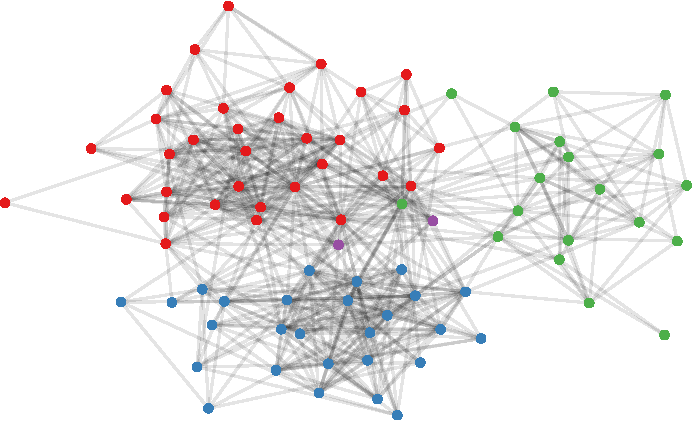
\includegraphics{draft_files/figure-latex/friendship-network-1} 

}

\caption{Friendship network of 81 faculty at a UK university. The vertices are labeled by school affiliation.}\label{fig:friendship-network}
\end{figure}
\end{example}

\hypertarget{probabilistic-models-for-graphs}{%
\subsection{Probabilistic Models for Graphs}\label{probabilistic-models-for-graphs}}

Given a sample or dataset, a typical analysis task is statistical inference, or the estimation of various parameters under the assumption that the data come from a random distribution or process.
These estimated parameters are often then used for making predictions or deriving insights about the population.
For example, when fitting a Gaussian mixture model, the data are first assumed to come from a mixture of Gaussians.
The model fitting process then involves estimating the means and standard deviations of each Gaussian component, along with the mixture weights.
The resulting model provides insight into where each mixture component is located, how disperse each component is, and how the data are distributed between the components, as well as a prediction indicating to which mixture a new observation belongs.
In order to perform a similar type of analysis for graphs, we must first define probability distributions from which such data can be sampled.

Within the scope of this work, we focus primarily on unweighted and undirected graphs without self-loops, with a brief discussion on generalizing these methods to weighted or directed graphs.
The adjacency matrix that describes these graphs is binary, symmetric, and hollow.
In this setting, a plausible model is to sample each edge independently from a Bernoulli distribution, i.e., \(A_{ij} \indep \Bernoulli(P_{ij})\) for some \(P_{ij} \in [0, 1]\) for each \(i < j\) (setting \(A_{ji} = A_{ij}\) since \(A\) is symmetric, and \(A_{ii} = 0\) since \(A\) is hollow).
Then similar to how the edges are compiled into an adjacency matrix \(A\), the edge probabilities can be compiled into an edge probability matrix \(P \in [0, 1]^{n \times n}\).
This type of graph model is defined as a \emph{Bernoulli random graph} (also called an inhomogeneous \(\ER\) graph).
If \(A\) is the adjacency matrix of a Bernoulli random graph with edge probability matrix \(P\), we denote \(A \sim \BG(P)\).
If the vertices and edge probabilities are sampled as a sequence of \(n\) i.i.d. random variables from probability distribution \(F\), then we denote \(A \sim \BG(F, n)\).

Statistical inference is not possible on a general Bernoulli random graph with arbitrary edge probabilities since the number of parameters (individual edge probabilities) is equal to the number of observations (presence or absence of an edge).
Additional structure must be introduced.
One such structured Bernoulli random graph model is the \(\ER\) graph, first proposed by \cite{Gilbert:1959}, which is defined as follows:

\begin{definition}[$\ER$ graph]
\label{def:erdos-renyi}
Let $P$ be an $n \times n$ matrix such that each $P_{ij} \equiv \theta \in [0, 1]$ is a constant. 
Then $A \sim \BG(P)$ is an $\ER$ graph. 
\end{definition}

\begin{example}[Maximum likelihood estimator for the $\ER$ graph]
One possible estimator for the lone parameter of an $\ER$ graph, $\theta$, is the maximum likelihood estimator, which is found by maximizing the log-likelihood function $\ell(\theta; A) = \log \theta \sum\limits_{i < j} A_{ij} + \log (1 - \theta) \sum\limits_{i < j} (1 - A_{ij})$. 
This can be solved directly by setting $\frac{d \ell}{d \theta} = 0$, which yields $\hat{\theta} = \frac{2 |E|}{n (n-1)}$.
\end{example}

\(\ER\) graphs lie on the opposite end of the spectrum in that they restrict the model to a single parameter, which does not result in a very interesting model or reflect many networks observed in real data.
Much work has been done in developing various Bernoulli random graph models that strike a balance between structure and flexibility.
Two common types of structure for graph models, that are of particular interest in this work, are edge probabilities based on latent communities \citep{doi:10.1080/0022250X.1971.9989788, NIPS2008_3578, Karrer_2011, 307cbeb9b1be48299388437423d94bf1}, called \emph{block models}, and edge probabilities based on positions in a latent space \citep{10.1007/978-3-540-77004-6_11, rubindelanchy2017statistical}, called \emph{latent space models}.

\begin{example}
Consider a graph in which the vertices represent a collection of $n$ planets with intelligent life sending out radio waves, and the existence of an edge between vertices $i$ and $j$ represents whether planets $i$ and $j$ have established contact.  
Since radio waves decay according to the inverse-square law, a plausible model for the edge probability between two vertices is 
$$P_{ij} = \frac{C \omega_i \omega_j}{d_{ij}^2}$$ 
where $\omega_i$ is the $i^{th}$ planet's radio signal strength, $d_{ij}$ is the Euclidean distance between planets $i$ and $j$, and $C$ is a normalizing constant. 
Let $P$ be the $n \times n$ matrix of these edge probabilities. 
Then $A \sim \BG(P)$ represents the network of planets that have made contact. 

To estimate $\omega = \Big[ \omega_1, \cdots, \omega_n \Big]^\top$ after observing $A$ and supposing that the relative locations of the planets as well as the normalizing constant $C$ are known, one approach might be maximum likelihood maximization. 
For simplicity, set $C = 1$. 
Then the log-likelihood function can be written as:
$$
\ell(\omega; A) = 
\sum_{i < j} A_{ij} \log \bigg( \frac{\omega_i \omega_j}{d_{ij}^2 -
\omega_i \omega_j} \bigg) + \log (d_{ij}^2 - \omega_i \omega_j) + const.
$$
The partial derivatives with respect to each $\omega_i$ are:
$$
\frac{\partial \ell}{\partial \omega_i} = \sum_{j \neq i} \frac{A_{ij}}{\omega_i} - \frac{\omega_j (1 - A_{ij})}{d_{ij}^2 - \omega_i \omega_j}.
$$
Setting the gradient to zero yields $n$ equations with $n$ unknowns, but it is not entirely obvious how to solve this system of equations. 
Alternatively, we can use gradient ascent or some other numerical optimization method, since this particular log-likelihood function is concave. 
\end{example}

\begin{definition}[Degree of a vertex]
\label{def:degree}
Let $G = (V, E)$ be an undirected graph with vertex set $V = \{v_1, ..., v_n\}$. 
$d_i$, the degree of vertex $v_i$ is the sum of the weights of edges that connect to $v_i$. 
If $G$ is unweighted, then $v_i$ is equivalently the number of edges that connect to $v_i$. 
If $G$ is represented by affinity or adjacency matrix $A$, then $d_i = \sum_j A_{ij}$. 

If $G$ is a Bernoulli random graph with edge probability matrix $P$, then the degree of each vertex $v_i$ is a random variable, and its expected value (also called expected degree) is $E[d_i] = \sum_j P_{ij}$. 
For example, the expected degree of each vertex of an $\ER$ graph with $n$ vertices and constant edge probability $p$ is $(n - 1) p$. 
\end{definition}

\hypertarget{contributions-of-this-work}{%
\subsection{Contributions of This Work}\label{contributions-of-this-work}}

In this work, we explore three types of block models, the stochastic block model, the degree corrected block model, and the popularity adjusted block model, as well as a family of latent space models called generalized random dot product graphs.

The contributions of this work are as follows.

In section \ref{sec:pabm-grdpg}, we show that, similar to how the stochastic block model and degree corrected block model are generalized random dot product graphs with specific latent structures, the popularity adjusted block model is also a generalized random dot product graph with a specific structure.
More specifically, we show that the popularity adjusted block model is a generalized random dot product graph in which the latent vectors are organized by community and each community in the latent space is defined by a \(K\)-dimensional subspace, where \(K\) is the number of communities in the model.
We then exploit this rigid and linear structure for community detection by applying sparse subspace clustering on the adjacency spectral embedding of the graph to infer the community labels.
We also propose a novel algorithm called orthogonal spectral clustering, which constructs an embedding for the popularity adjusted block model which forces the communities to lie on \emph{orthogonal} subspaces.
Finally, we propose a spectral decomposition based parameter estimation algorithm for the popularity adjusted block model.
All three algorithms have consistency properties that result in zero error with increasing graph size.

In section \ref{sec:mbm}, we extend the latent structures of the stochastic block model, degree corrected block model, and popularity adjusted block model to nonlinear latent structures.
Instead of points, line segments, and subspaces, we propose the manifold block model which is a class of generalized random dot product graph in which the latent vectors lie on one of \(K\) manifolds.
In the case of nonintersecting manifolds, we show that a clustering algorithm based on a nearest algorithms graph approach on an embedding is consistent, resulting in zero clustering error for large graphs, as long as the latent vectors are sampled from the manifolds densely
In the case of intersecting manifolds, we propose the \(K\)-curves algorithm, which is a type of batch coordinate ascent algorithm which alternates between fitting manifolds to the embedding and reassigning clusters based on proximity to the manifolds.

\newpage

\hypertarget{preliminaries}{%
\section{Preliminaries}\label{preliminaries}}

\hypertarget{sec:blockmodel}{%
\subsection{Block Models for Community Detection}\label{sec:blockmodel}}

Network analysis is often concerned with community detection.
This has motivated statisticians to develop random graph models with inherent community structure in which the probability of an edge between vertices \(v_i\) and \(v_j\) depend on the community assignments \(z_i\) and \(z_j\).
More formally, one assigns each vertex \(v_i\) a community label \(z_i \in \{1, ..., K\}\) and assumes a Bernoulli random graph in which \(P_{ij} = g(z_i, z_j, \theta_i, \theta_j)\) for some function \(g: \{1, ..., K\}^2 \times \mathbb{R}^d \times \mathbb{R}^d \to [0, 1]\) and \(\theta_i \in \mathbb{R}^d\) is a vector of real-valued parameters associated with each vertex.
Within the context of this work, we will call such models \emph{block models}.
This type of model framework allows us to frame the goal of community detection as a statistical inference problem:
come up with estimators for the true community labels, up to permutation.

In this section, we explore the three main types of block models:
the stochastic block model \citep{doi:10.1080/0022250X.1971.9989788}, the degree corrected block model \citep{Karrer_2011}, and the popularity adjusted block model \citep{307cbeb9b1be48299388437423d94bf1}.
The main focus is on how these models are connected, particularly in how they are nested models \citep{Noroozi2022}, as well as community detection and parameter estimation via likelihood maximization.
We will later return to these block models and the relationship to another class of random graph models in sections \ref{sec:grdpg} and \ref{sec:pabm-grdpg}.

\hypertarget{sec:sbm}{%
\subsection{The Stochastic Block Model}\label{sec:sbm}}

The stochastic block model (SBM) \citep{doi:10.1080/0022250X.1971.9989788} is the simplest of the three block models and assumes that each pair of communities \((k, \ell)\) has a constant edge probability \(\theta_{k \ell}\).
We now give the formal definition of the SBM within the context of Bernoulli random graphs:

\begin{definition}[Stochastic block model]
\label{def:sbm}
Let $G = (V, E)$ be a Bernoulli random graph with $n$ vertices, described by random adjacency matrix $A$. 
Let $K \geq 1$ be an integer and $\theta_{k \ell} \in [0, 1]$ for each $k, \ell \in \{1, ..., K\}$ (if $G$ is undirected, then $\theta_{k \ell} = \theta_{\ell k}$). 
Let $z_1, ..., z_n \in \{1, ..., K\}$ be community labels associated with each vertex. 
If the edge probability matrix $P$ for this graph is such that 
$P_{ij} = \theta_{z_i, z_j}$ and $A \sim \BG(P)$, then $G$ is a stochastic block model. 
\end{definition}

There are a few conventions for exactly how a graph is sampled as an SBM.
Within the context of this work, we assume that for a particular SBM, the number of communities, \(K\), and the community edge probabilities, \(\theta_{k \ell}\), are fixed.
Then some possible ways of sampling from an SBM are as follows:

\begin{enumerate}
\def\labelenumi{\arabic{enumi}.}
\tightlist
\item
  Let the size of the graph, \(n\), be fixed.
  Then each vertex \(v_i\), and its corresponding label, \(z_i\), are also fixed, in addition to the pairwise community edge probabilities \(\{\theta_{k \ell}\}_K\), which are all treated as model parameters.
  Under this sampling scheme, there is no notion of increasing \(n\).
\item
  The vertices and edges are sampled in sequence, and we suppose that each vertex \(v_i\) comes with a corresponding label, \(z_i\), which determines its edge probabilities to the other vertices.
  Under this sampling scheme, there is no assumed distribution on the labels, which are treated as fixed parameters rather than random variables, along with \(\{\theta_{k \ell}\}_K\), but there is a notion of increasing sample size \(n\), which allows for asymptotics.
\item
  The vertices are sampled in sequence, and each label, \(z_i\), is sampled as \(z_1, ..., z_n \iid \Multinomial(\alpha_1, ..., \alpha_K)\), \(\sum_k^K \alpha_k = 1\).
  The edge probabilities are then determined by the sample \(\{z_i\}\) and the parameters \(\{\theta_{k \ell}\}_K\).
  Under this sampling scheme, both the edges and the labels are random, with fixed parameters \(\alpha = \Big[ \alpha_1, \cdots, \alpha_K \Big]^\top\) and \(\{\theta_{k \ell}\}_K\).
\end{enumerate}

We use the notation \(A \sim \SBM(z, \{\theta_{k \ell}\}_K)\) for the first two sampling schemes, and we use \(A \sim \SBM(\alpha, \{\theta_{k \ell}\}_K)\) for the third.

An extension to these include Bayesian models in which there are prior distributions for the parameters, e.g., each \(\theta_{k \ell}\) has a prior distribution with support \([0, 1]\), such as \(\theta_{k \ell} \sim \Betadist(a_{k \ell}, b_{k \ell})\), and the mixture parameters \(\alpha\) has a prior distribution on the \(K-1\) simplex, such as \(\alpha \sim \mathrm{Dirichlet}(\beta_1, ..., \beta_K)\).

\begin{example}[Stochastic block model with $K = 2$ communities]
\label{ex:assort-sbm}
We construct an SBM with two communities in which $\theta_{11} = 1/2$, $\theta_{12} = 1/8$, and $\theta_{22} = 1/4$. 
Note that in this example, the within-community edge probabilities are greater than the between-community edge probability. 
A realization of this graph with $n_1 = n_2 = 32$ (where $n_k = |\{v_i : z_i = k\}|$) is illustrated in figure \ref{fig:assort-sbm}.

\begin{figure}[H]

{\centering 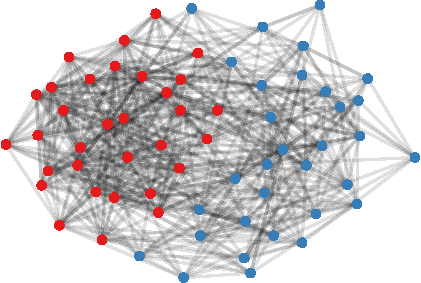
\includegraphics{draft_files/figure-latex/assort-sbm-1} 

}

\caption{Two-community stochastic block model with $\theta_{11}=1/2$, $\theta_{22}=1/4$, and $\theta_{12} = \theta_{21} = 1/8$.}\label{fig:assort-sbm}
\end{figure}
\end{example}

In most conceptions of block models, the within-community edge probability is greater than the between-community edge probability, as in example \ref{ex:assort-sbm}.
This reflects the general intuition that pairs within the same community are more likely to be connected than pairs between two different communities.
For instance, in the UK faculty friendship network in example \ref{ex:uk-faculty}, it is natural to expect that faculty within the same school are more likely to be friends than faculty from two different schools, and a cursory look at the visualization of the network appears to confirm this.
However, SBMs are not necessarily restricted to this type of community structure.
We could just as easily construct an example in which \(\theta_{11}\) and \(\theta_{22}\) are less than \(\theta_{12}\).
Within the context of block models, we say that a graph is \emph{assortative} if \(P\) is positive semidefinite and \emph{disassortative} otherwise, which roughly correspond to communities with higher within-community edge probabilities and lower between-community edge probabilities, respectively.
For example, the SBM in example \ref{ex:assort-sbm} is assortative and has edge probability matrix \(P\) that is rank 2 with nonzero eigenvalues \(n (\frac{3}{8} \pm \frac{\sqrt{2}}{8}) > 0\).
In the following example, we describe a network which can be modeled as a disassortative SBM.

\begin{example}[Dating network as a disassortative stochastic block model]
\label{ex:sbm-dating}
Consider an undirected graph in which each vertex $v_i$ represents users of an online dating service, each label $z_i$ represents the user's gender, and each edge represents a successful match between pairs of users. 
For simplicity, we will restrict the labels to female and male (denoted as $1$ and $2$). 
If we model this as an SBM, then $\theta_{11}$ is the probability of a match between two female users, $\theta_{22}$ is the probability of a match between two male users, and $\theta_{12} = \theta_{21}$ is the probability of a match between a female user and a male user. Based on trends in the United States \citep{gallup-lgbt}, 
a plausible set of edge probabilities is $\theta_{11} = \theta_{22} = 0.02$ and $\theta_{12} = 0.2$, which are used in the sample visualized in figure \ref{fig:dating-sbm}, along with $\alpha_1 = \alpha_2 = 1/2$ and $n = 64$.

\begin{figure}[H]

{\centering 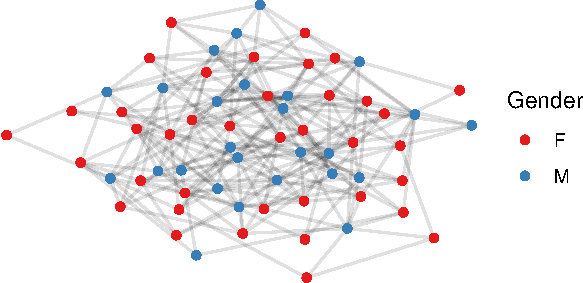
\includegraphics{draft_files/figure-latex/dating-sbm-1} 

}

\caption{Stochastic block model of a dating network. This model is disassortative.}\label{fig:dating-sbm}
\end{figure}
\end{example}

\begin{example}[Assortativity and disassortativity of the two-community SBM]
\label{ex:sbm-assortativity}
Let $P$ be the $n \times n$ probability matrix of a two-community SBM. 
Then $rank(P) = 2$, and its two nonzero eigenvalues are:

$$
\lambda = \frac{n}{2} \bigg( 
\theta_{11} + \theta_{22} \pm 
\sqrt{(\theta_{11} - \theta_{22})^2 + 4 \theta_{12}^2} 
\bigg).
$$
The first eigenvalue is always positive. 
The second eigenvalue is positive if $\theta_{11} \theta_{22} > \theta_{12}^2$. 
Thus, $P$ describes an assortative SBM if $\theta_{11} \theta_{22} > \theta_{12}^2$ or 
a disassortative SBM if $\theta_{11} \theta_{22} < \theta_{12}^2$. 
This corresponds to the high-level understanding of assortativity and disassortativity based on whether within or between community edge probabilities are greater. 
\end{example}

One approach to statistical inference for the SBM is likelihood maximization.
The log-likelihood function can be written as:
\begin{equation}
\label{eq:sbm-loglik}
\ell(z, \theta; A) = \sum_{i < j} \sum_{k, \ell} z_{ik} z_{j \ell} \big( 
A_{ij} \log \theta_{k \ell} - (1 - A_{ij}) \log (1 - \theta_{k \ell}) \big),
\end{equation}
where \(z_{ik} = I(z_i = k)\). If the labels are drawn from a multinomial distribution, then that can also be incorporated into the complete-data log-likelihood:
\begin{equation}
\label{eq:sbm-loglik-full}
\ell(z, \theta, \alpha; A) = \sum_k \sum_i z_{ik} \log \alpha_k + 
\sum_{i < j} \sum_{k, \ell} z_{ik} z_{j \ell} \big( 
A_{ij} \log \theta_{k \ell} - (1 - A_{ij}) \log (1 - \theta_{k \ell}) \big).
\end{equation}

The SBM is a type of mixture model, and like most classical mixture models and clustering problems, likelihood maximization is NP-hard.
But because the SBM is a mixture model, a candidate algorithm for finding a (local) maximum of the likelihood is the widely studied expectation maximization (EM) algorithm \citep{10.2307/2984875}.
However, due to the \(z_{ik} z_{j \ell}\) interaction terms, the expectation step cannot be solved in closed form \citep{kolaczyk2014statistical}.
While the labels are drawn independently, they are not necessarily conditionally independent.
Nevertheless, making the conditional independence relaxation allows us to write the expectation and maximization steps in closed form.
As an example, we write the EM algorithm for the likelihood function in equation \eqref{eq:sbm-loglik} in algorithm \ref{algo:sbm-em}.

\begin{algorithm}
\label{algo:sbm-em}
\setstretch{1.5}
\DontPrintSemicolon
\SetAlgoLined
\KwData{Adjacency matrix $A$, number of communities $K$}
\KwResult{Estimated community label probabilities $\{\pi_{ik}\}$ for which each $\pi_{ik} = P(z_i = k \mid A)$, estimated community edge probabilities $\{\hat{\theta}_{k \ell}\}_K$}
\caption{Approximate EM algorithm for the SBM}
Initialize $\{\pi_{ik}\}$, $\{\theta_{k \ell}\}$.\;
\While{$\|\nabla \ell\| > \epsilon$} {
\For {$i = 1, ..., n$} {
\For {$k = 1, ..., K$} {
E-step: $\pi_{ik} \propto \exp \bigg( \sum_{j \neq i} \sum_{\ell} \pi_{j \ell} (A_{ij} \log \hat{\theta}_{k \ell} + (1 - A_{ij}) \log (1 - \hat{\theta}_{k \ell})) \bigg)$.\;
M-step: $\hat{\theta}_{k \ell} = \frac{\sum_{i < j} A_{ij} \pi_{ik} \pi_{j \ell}}{\sum_{i < j} \pi_{ik} \pi_{j \ell}}$.\;
}
}
}
\end{algorithm}

Applying algorithm \ref{algo:sbm-em} to example \ref{ex:assort-sbm} with initial guesses of \(\pi_{ik} = 0.5\) for each \(i, k\), \(\hat{\theta}_{11} = \hat{\theta}_{22} = 0.9\), and \(\hat{\theta}_{12} = 0.1\) results in a community detection error rate of 4.7\% and parameter estimates \(\hat{\theta}_{11} = 0.503\), \(\hat{\theta}_{22} = 0.241\), and \(\hat{\theta}_{12} = 0.109\), compared to the true parameters \(\theta_{11} = 0.5\), \(\theta_{22} = 0.25\), and \(\theta_{12} = 0.125\).
The same algorithm applied to example \ref{ex:sbm-dating}, which is a disassortative model, using initial guesses of \(\pi_{ik} = 0.5\), \(\hat{\theta}_{11} = \hat{\theta}_{22} = 0.1\), and \(\hat{\theta}_{12} = 0.9\), results in a community detection error rate of 0\% and parameter estimates \(\hat{\theta}_{11} = 0.034\), \(\hat{\theta}_{22} = 0.018\), and \(\hat{\theta}_{12} = 0.201\), compared to the true parameters \(\theta_{11} = \theta_{22} = 0.02\) and \(\theta_{12} = 0.2\).

\hypertarget{sec:sparsity}{%
\subsection{Random Graph Models and Sparsity}\label{sec:sparsity}}

So far, we have described \emph{dense} Bernoulli random graphs.
For such models, as the sample size \(n\) increases, the expected degree of each node grows linearly.
For example, consider the SBM with the third sampling setup described in section \ref{sec:sbm}.
Then the expected degree of vertex \(v_i\) is
\[
\begin{split}
E[d_i] & = \sum_j P_{ij} \\
& = \sum_{j \neq i} \theta_{z_i, z_j} \\ 
& = \Big( \sum_k n_k \theta_{z_i, k} \Big) - \theta_{z_i, z_i} \\
& = n \Big( \sum_k \alpha_k \theta_{z_i, k} \Big) - \theta_{z_i, z_i} \\
& = O(n).
\end{split}
\]

In many real networks, the degree of each vertex often does not grow proportionally with the size of the network.
To account for this, a sparsity factor \(\rho_n \in (0, 1]\) is introduced in the edge probabilities, i.e., \(P_{ij} \leftarrow \rho_n P_{ij}\), for some sequence \(\{\rho_n\}\) such that \(\lim\limits_{n \to \infty} \rho_n = 0\).\\
For example, a sparse SBM has edge probabilities \(P_{ij} = \rho_n \theta_{z_i, z_j}\), for which we use the notation \(A \sim \SBM(z, \{\theta_{k \ell}\}_K; \rho_n)\) or \(A \sim \SBM(\alpha, \{\theta_{k \ell}\}_K; \rho_n)\), depending on whether we treat the labels as random or fixed.
Then the expected degree grows as \(O(n \rho_n)\) instead of linearly as \(O(n)\).
For the sake of unifying the sparse and dense regimes, we also allow for the special case \(\rho_n = 1\) and include the sparsity factor throughout, unless otherwise stated.
Finally, we also note that while \(\rho_n\) limits the rate of growth of the expected degree, our theoretical results still require \(n \rho_n\) to diverge to infinity, albeit at a slower rate than \(O(n)\).
In general, for consistency in estimation and inference, most results on Bernoulli random graphs require \(n \rho_n = \omega \big( (\log n)^c \big)\) for some \(c > 1\).
(See \cite{JMLR:v18:16-480}, \cite{https://doi.org/10.48550/arxiv.2106.09840}, and \cite{rubindelanchy2017statistical} for further discussion.)

\hypertarget{sec:dcbm-pabm}{%
\subsection{Generalizations of the Stochastic Block Model: The Degree Corrected Block Model and the Popularity Adjusted Block Model}\label{sec:dcbm-pabm}}

The SBM assumes homogeneity within each community.
In particular, in the SBM, each vertex's expected degree and affinity toward each community depends only on its community label.
The degree corrected block model (DCBM) and popularity adjusted block model (PABM) are generalizations of the SBM that address these limitations.
In particular, the DCBM allows each vertex to have an expected degree independent of its label, and the PABM allows each vertex to have edge probabilities to each community independent of its own label.
We also show that the DCBM is a special case of the PABM and that the SBM, DCBM, and PABM are nested models.

\begin{definition}[Degree corrected block model]
\label{def:dcbm}
Let $G = (V, E)$ be a Bernoulli random graph with $n$ vertices, described by random adjacency matrix $A$. 
Let $K \geq 1$ be an integer and $\theta_{k \ell} \in [0, 1]$ for each $k, \ell \in \{1, ..., K\}$ (if $G$ is undirected, then $\theta_{k \ell} = \theta_{\ell k}$), as in the SBM. 
Let $z_1, ..., z_n \in \{1, ..., K\}$ be community labels associated with each vertex. 
In addition, each vertex $v_i$ has a degree correction parameter $\omega_i \in [0, 1]$. 
If the edge probability matrix $P$ for this graph is such that $P_{ij} = \rho_n \theta_{z_i, z_j} \omega_i \omega_j$ and $A \sim \BG(P)$, then $G$ is a degree corrected block model. 
We use the notation $A \sim \DCBM(z, \{\theta_{k \ell}\}_K, \omega; \rho_n)$ to denote a random adjacency matrix drawn from the DCBM with labels $z$, base edge probabilities $\{\theta_{k \ell}\}_K$, and degree correction factors $\omega$. 
Under the sampling scheme in which the labels are drawn from a multivariate distribution with class probabilities $\alpha$, we use the notation $A \sim \DCBM(\alpha, \{\theta_{k \ell}\}_K, \omega; \rho_n)$.
\end{definition}

\begin{example}[Dating network as a disassortative DCBM]
\label{ex:dcbm-dating}
In example \ref{ex:sbm-dating}, we modeled an online dating network as an SBM in which the vertices correspond to individuals, the communities correspond to genders, and edges correspond to whether the online dating service successfully matched pairs of individuals. 
In this model, we assume that for each pair of genders, there is a constant probability of a match. 
This does not take into account that some individuals are more likely to form connections than others, based on each individual's activity on the online service or popularity with other users. 
Modeling this as a DCBM allows us to take this into account by adjusting each user's degree by $\omega_i$. 
The following is a visualization of the network from example \ref{ex:sbm-dating} modified as a DCBM with parameters $\theta_{11} = \theta_{22} = 0.03$, $\theta_{12} = 0.3$, each $\omega_i$ drawn uniformly between $1/3$ and $1$, and $\rho_n \equiv 1$. 

\begin{figure}[H]

{\centering 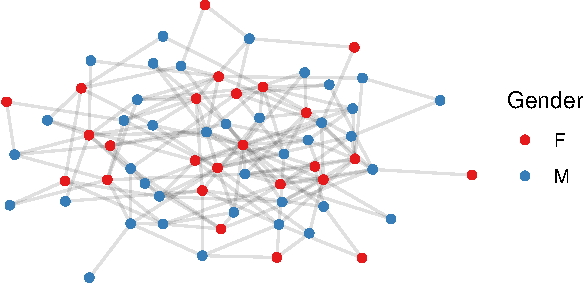
\includegraphics{draft_files/figure-latex/dating-dcbm-1} 

}

\caption{A dating network modeled as a DCBM. This model is disassortative.}\label{fig:dating-dcbm}
\end{figure}
\end{example}

The DCBM allows for each vertex to have its own expected degree while still maintaining community structure.
However, it still assumes that each vertex within a community has the same relative propensity to connect to each community.
For example, going back to the dating network in examples \ref{ex:sbm-dating} and \ref{ex:dcbm-dating}, the models assume that each individual is ten times more likely to connect with a member of the opposite sex than with a member of the same sex.
The popularity adjusted block model \citep{307cbeb9b1be48299388437423d94bf1} allows each vertex to have its own affinity toward each community.
In the dating network example, the PABM allows us to model each individual's preferences instead of using population level averages.

\begin{definition}[Popularity adjusted block model]
\label{def:pabm}
Let $G = (V, E)$ be an undirected Bernoulli random graph with $n$ vertices, described by random adjacency matrix $A$. 
Let $K \geq 1$ be an integer that describes the number of communities, and let 
$z_1, ..., z_n \in \{1, ..., K\}$ be community labels associated with each vertex. 
Suppose that each vertex $v_i$ has $K$ popularity parameters $\lambda_{i1}, ..., \lambda_{iK}$ for which each $\lambda_{ik}$ describes $v_i$'s affinity toward community $k$. 
Then if the edge probability matrix $P$ for this graph is such that $P_{ij} = \rho_n \lambda_{i, z_j} \lambda_{j, z_i}$ and $A \sim \BG(P)$, then $G$ is a popularity adjusted block model.
We use the notation $A \sim \PABM(z, \{\lambda_{i, k}\}_K; \rho_n)$ to denote a random adjacency matrix drawn from the PABM with labels $z$ and popularity parameters $\{\lambda_{i, k}\}_K$. 
Under the sampling scheme in which the labels are drawn from a multivariate distribution with class probabilities $\alpha$, we use the notation $A \sim \PABM(\alpha, \{\lambda_{i, k}\}_K; \rho_n)$. 
\end{definition}

\begin{example}[Dating network as a PABM]
\label{ex:pabm-dating}
In examples \ref{ex:sbm-dating} and \ref{ex:dcbm-dating}, we modeled an online dating network as a SBM and a DCBM, in which the vertices correspond to individuals, the communities correspond to genders, and the edges represent whether the online dating service successfully matched pairs of individuals. 
In these models, it is assumed that all individuals have the same sexual orientation. 
Using the parameters specified in these examples, we assume that each individual is 10 times more likely to match with a member of the opposite sex compared to a member of the same sex. 
The PABM allows us to model each individual's sexual orientation. 
Figure \ref{fig:dating-pabm} is a visualization of the online dating network modeled as a PABM in which the popularity parameters are drawn as $\lambda_{ik} \sim \Betadist(1, 6)$ if $z_i = k$ and $\lambda_{ik} \sim \Betadist(2, 2)$ if $z_i \neq k$. 
Like in the SBM and DCBM examples, the average edge probability between genders is approximately ten times that of the average edge probability within genders, but unlike in the SBM and DCBM examples, each individual has its own affinity toward each gender. 

\begin{figure}[H]

{\centering 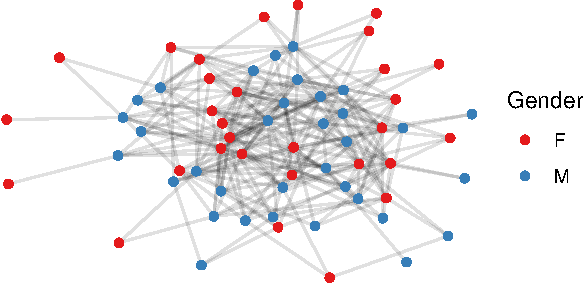
\includegraphics{draft_files/figure-latex/dating-pabm-1} 

}

\caption{A dating network modeled as a PABM. This model is disassortative.}\label{fig:dating-pabm}
\end{figure}
\end{example}

\begin{remark}
Unlike the SBM (when excluding the sparsity factor), each DCBM and PABM is not unique and therefore non-identifiable. 
For example, in the case of the DCBM, doubling each $\theta_{k \ell}$ and dividing each $\omega_i$ by $\sqrt{2}$ results in the same edge probability matrix. 
\citet{Karrer_2011} suggest imposing the constraint $\sum_{i : z_i = k} \omega_i = 1$ for each $k \in \{1, ..., K\}$, but other similar constraints can be used to enforce uniqueness, such as $\max_i \omega_i = 1$ and $\min_i \omega_i = 0$. 
Despite the lack of uniqueness without constraints, a naive EM type algorithm similar to the one in section \ref{sec:sbm} results in high community detection accuracy for most realizations of the DCBM and PABM, although it is not clear what its asymptotic properties are or whether there are any theoretical guarantees. 
Likewise, it is not immediately obvious how to approach the estimation of the $\theta_{k \ell}$'s, $\omega_i$'s, or $\lambda_{ik}$'s due to their non-uniqueness. 
\citet{noroozi2019estimation} suggest focusing estimation on the edge probability matrix $P$ instead of the individual parameters to avoid this ambiguity. 
Applying an EM algorithm similar to algorithm \ref{algo:sbm-em} adapted for the DCBM to example \ref{ex:dcbm-dating} results in 84\% accuracy, and applying a similar EM algorithm adapted for the PABM to example \ref{ex:pabm-dating} results in 97\% accuracy, but they fail to capture the original (which are not necessarily ``true'') parameters. 
\end{remark}

\hypertarget{sec:hierarchy}{%
\subsection{A Hierarchy of Block Models}\label{sec:hierarchy}}

The PABM, DCBM, and SBM are nested models, that is, the SBM is a special case of the DCBM which in turn is a special case of the SBM.
In this section, these connections are made explicit, and we explore the implications for modeling.
For ease of notation, throughout this section the rows and columns of \(P\) are assumed to be organized by community in increasing order, i.e., the first \(n_1\) rows and columns of \(P\) correspond to community \(1\), the next \(n_2\) rows and columns correspond to community \(2\), etc.
We use the notation \(P^{(k \ell)} = (P^{(\ell k)})^\top\) to denote the block of \(P\) that corresponds to the edges between communities \(k\) and \(\ell\).
In section \ref{sec:pabm-grdpg}, we will deal with this notation and convention more carefully.
For additional details on the connections among the SBM, DCBM, and PABM, refer to \citet{Noroozi2022}.

To see that the SBM is a special case of the DCBM, we can simply restrict the degree parameters \(\omega_i\) to all be a constant value, e.g., \(\omega_i \equiv 1\).
But in order to better understand the relationship between these two models, we will break down the models further.

Define \(B\) as the \(K \times K\) matrix of edge probabilities between pairs of communities in the SBM.
Then \(B_{k \ell} = \theta_{k \ell}\) and \(P_{ij} = \theta_{z_i, z_j} = B_{z_i, z_j}\).
We can further show that block \(P^{(k \ell)}\) can be written as \(P^{(k \ell)} = e^{(k)} B_{k \ell} (e^{(\ell)})^\top\) where \(e^{(k)}\) is the \(1\)-vector of dimension \(k\).
Since \(B_{k \ell}\) is a scalar, \(P^{(k \ell)} = e^{(k)} B_{k \ell} (e^{(\ell)})^\top\) is a singular value decomposition of a rank 1 matrix and thus each block \(P^{(k \ell)}\) is rank 1.
Then we can see that the entire edge probability matrix can be written as
\[P = Z B Z^\top\]
and \(Z\) is an \(n \times K\) matrix in which \(Z_{ik} = I(z_i = k) = z_{ik}\). Thus, if \(B\) is full rank, i.e., \(\rank(B) = K\), then \(P\) is also rank \(K\).

To extend the SBM to the DCBM, we replace \(e^{(k)}\) with the vector \(\omega^{(k)}\) which contains the degree parameters of vertices in community \(k\).
Then for the DCBM, \(P^{(k \ell)} = \omega^{(k)} B_{k \ell} (\omega^{(\ell)})^\top\).
Similar to the SBM, this is a singular value decomposition of a rank 1 matrix.
The full edge probability matrix can be written as
\[P = (\Omega Z) B (\Omega Z)^\top\]
for \(\Omega = \diag(\omega)\).
Since \(\Omega\) is diagonal, we again have that \(\rank(P) = K\) (again, assuming that \(B\) is full rank).
Thus, the dimensionality of the DCBM is the same as the SBM, and to restrict the DCBM to the PABM, let \(\Omega = I\).

To extend the DCBM to the PABM, we note that the \(k \ell\)\textsuperscript{th} block of the edge probability matrix can be written as \(P^{(k \ell)} = \lambda^{(k \ell)} (\lambda^{(\ell k)})^\top\) where \(\lambda^{(k \ell)} \in \mathbb{R}^{n_k}\) is the vector of popularity parameters belonging to vertices in community \(k\) that point to community \(\ell\), i.e., \(\lambda^{(k \ell)}_i = \lambda_{i + \sum_{s=1}^{k-1} n_s, \ell}\).
Similar to how \(\omega^{(k)}\) is a sub-vector of \(\omega\)
To match this decomposition with the one for the DCBM, we can fix each \(B_{k \ell} \equiv 1\) and write \(P^{(k \ell)} = \lambda^{(k \ell)} B_{k \ell} (\lambda^{(\ell k)})^\top\).
Restricting each \(\lambda^{(k \ell)} = \omega^{(k)}\) reduces the PABM to the DCBM.
To write out the full edge probability matrix of the PABM, let \(\Lambda^{(k)} =\begin{bmatrix} \lambda^{(k1)} & \cdots & \lambda^{(kK)} \end{bmatrix}\) and \(X = \blockdiag(\Lambda^{(1)}, ..., \Lambda^{(K)})\).
Then for some \(K^2 \times K^2\) permutation matrix \(\Pi\),
\[P = X \Pi X^\top.\]
From this decomposition, we can see that unlike the SBM and DCBM, \(\rank(P) = \rank(X) = K^2\).
We will explore this decomposition of the edge probability matrix of the PABM in more detail in section \ref{sec:pabm-grdpg}.

The full hierarchy of nested block models is summarized in table \ref{tab:hierarchy}.

\begin{table}

\caption{\label{tab:hierarchy}Summary of an hierarchical or nested view of block momdels.}
\centering
\begin{tabular}[t]{l|l|l|l|l}
\hline
Model & Parameters & $\mathrm{rank}(P)$ & Matrix Decomposition & Reduction to simpler model\\
\hline
SBM & $K (K-1) / 2$ & $K$ & $P = Z B Z^\top$ & \\
\hline
DCBM & $K (K-1) / 2 + n$ & $K$ & $P = (\Omega Z) B (\Omega Z)^\top$ & $\omega = e$\\
\hline
PABM & $n K$ & $K^2$ & $P = X \Pi X^\top$ & $\lambda_{ik} = \omega_i \sqrt{\theta_{z_i, k}}$\\
\hline
\end{tabular}
\end{table}

\newpage

\hypertarget{sec:grdpg}{%
\subsection{The Generalized Random Dot Product Graph}\label{sec:grdpg}}

In the Bernoulli random graph, the edge probability matrix \(P\) is of size \(n \times n\), but when \(K \ll n\), the structure of \(P\) is much simpler than its dimensions imply.
In particular, \(P\) is rank \(K\) in the SBM and DCBM and rank \(K^2\) in the PABM.
This property lends these block models to be analyzed as another family of Bernoulli random graphs with low rank called the random dot product graph (RDPG) and generalized random dot product graph (GRDPG).
In these models, \(P\) is decomposed into an outer product of two low-rank data matrices.

\begin{definition}[Generalized random dot product graph]
\label{def:grdpg}
Let $p \geq 1$ and $q \geq 0$ be integers. 
Define $I_{p,q}$ as the block diagonal matrix $I_{p,q} = \Bigl[\begin{smallmatrix} I_{p} & 0 \\ 0 & - I_{q} \end{smallmatrix} \Bigr]$ where $I_p$ and $I_q$ are the identity matrices of dimensions $p \times p$ and $q \times q$ respectively. 
Denote $d = p + q$ and let $\mathcal{X}$ be the subset of $\mathbb{R}^d$ such that, for any $x, y \in \mathcal{X}$, we have $x^\top I_{p,q} y \in [0, 1]$. 
Let $X = \Big[ x_1 \mid \cdots \mid x_n \Big]^\top$ be an $n \times d$ matrix with rows $x_i \in \mathcal{X}$. 
A graph $G$ with adjacency matrix $A$ is said to be a generalized random dot product graph with latent positions $X$, sparsity parameter $\rho_n$, and signature $(p, q)$ if $A \sim \BG(P)$ where the edge probability matrix $P$ is given by $P = \rho_n X I_{p,q} X^\top$, i.e., the entries of $P$ are of the form $P_{ij} = \rho_n x_i^\top I_{p,q} x_j$. 

We use the notation $A \sim \GRDPG_{p,q}(X; \rho_n)$ to denote a random adjacency matrix $A$ drawn from latent positions $X$, sparsity parameter $\rho_n$, and signature $(p, q)$. If the $n$ vectors in $X$ are drawn from probability distribution $F$ on support $\mathcal{X}$, we use the notation $A \sim \GRDPG_{p,q}(F; \rho_n)$. 

If $q = 0$ and so $d = p$, (i.e., $P$ is positive semidefinite), then we call this a random dot product graph. 
In this case, we use the notation $A \sim \RDPG(X; \rho_n)$ and $A \sim \RDPG(F; \rho_n)$. 
\end{definition}

\begin{definition}[Indefinite orthogonal group]
\label{def:indefinite}
The indefinite orthogonal group with signature $(p, q)$ is
the set $\{Q \in \mathbb{R}^{d \times d} \colon Q I_{p, q} Q^{\top} = I_{p, q}\}$,
denoted as $\mathbb{O}(p, q)$. Here $d = p + q$. 
\end{definition}

\begin{remark}
\label{rem:non_identifiable}
The latent vectors that produce $X I_{p,q} X^\top = P$ are not unique
\citep{rubindelanchy2017statistical}.
More specifically, if $P_{ij} = x_i^\top I_{p, q} x_j$, then for any $Q \in \mathbb{O}(p, q)$ we also have 
$(Q x_i)^\top I_{p, q} (Q x_j) = x_i^\top (Q^\top I_{p, q} Q) x_j = x_i^\top I_{p, q} x_j = P_{ij}$. 
Unlike in the RDPG case, transforming the latent positions via multiplication by $Q \in \mathbb{O}(p, q)$ does not necessarily maintain interpoint angles or distances.
\end{remark}

Now that we defined the GRDPG as a generative model for Bernoulli random graphs,
we need a method for estimation.
We can use Adjacency Spectral Embedding (ASE) \citep{doi:10.1080/01621459.2012.699795} to recover the latent vectors of a GRDPG.
This procedure consists of taking the spectral decomposition of \(A\) and keeping the \(p + q\) largest eigenvalues (in modulus) and corresponding eigenvectors of \(A\).

\begin{definition}[Adjacency spectral embedding]
\label{def:ase}
Let $A$ be an $n
\times n$ adjacency matrix and denote the
eigendecomposition of $A$ as
$$A = \sum_{i} \hat{\lambda}_i \hat{v}_i \hat{v}_i^{\top}, \quad
\text{where} \,\,
|\hat{\lambda}|_1 \geq |\hat{\lambda}_2| \geq \dots \geq
|\hat{\lambda}_n|.$$
Let $\hat{D}$ be a diagonal matrix whose diagonal entries are
the eigenvalues $\{\hat{\lambda}_i\}_{i=1}^{d}$ arranged in decreasing values (not in
decreasing modulus) and let $\hat{V}$ be the $n \times d$ matrix whose
columns are the corresponding eigenvectors $\{\hat{v}_i\}_{i=1}^{d}$
arranged in the same order as the diagonal entries of $\hat{D}$. Now
define $\hat{X} = \hat{V} |\hat{D}|^{1/2}$ where the $|\cdot|$
operation is applied elementwise to the entries of $\hat{D}$. Then
$\hat{X}$ serves as an estimate of $X$, up to some non-identifiable
orthogonal transformation $Q$ as described in
remark~\ref{rem:non_identifiable} and definition~\ref{def:indefinite};
see \citet{rubindelanchy2017statistical} for further details.
\end{definition}

\citet{doi:10.1080/01621459.2012.699795} and \citet{rubindelanchy2017statistical} showed that the ASE is consistent in estimating the latent vectors, up to an indefinite orthogonal transformation.
More specifically, for sparsity parameters such that \(n \rho_n = \omega (\log^{4 c} n)\) for some constant \(c > 1\) and indefinite orthogonal transformation \(Q \in \mathbb{O}(p, q)\),
\[\max_i \|Q \hat{x}_i - x_i \| = O_P \bigg( \frac{\log^c n}{n^{1/2}} \bigg)\]
where \(x^\top\) and \(\hat{x}^\top\) are the rows of \(\hat{X}\) (from the ASE) and \(X\), respectively.

\begin{example}
Suppose that latent vectors for an RDPG are drawn from the curve 
$x(t) = \Big[ t^2, 2 t (t-1) \Big]^\top$, $t \in [0, 1]$. 
Let $x_i = x(t_i)$. 
Then for each $i < j$, the edges are drawn as $A_{ij} \indep \Bernoulli(x_i^\top x_j)$. 
If after observing $A$, we wish to estimate the curve, the ASE provides an estimator in which the estimated latent vectors converge to the curve, up to an orthogonal transformation (figure \ref{fig:ase-example}). 

\begin{figure}[H]

{\centering 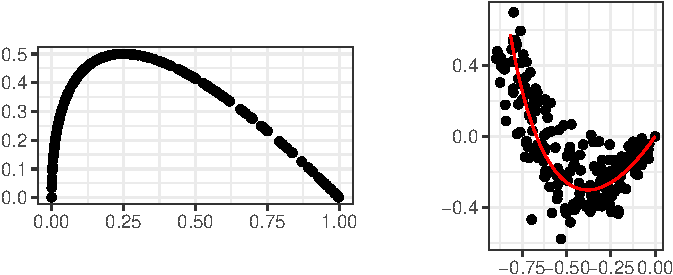
\includegraphics{draft_files/figure-latex/ase-example-1} 

}

\caption{200 points drawn from a curve (left), and the ASE of an adjacency matrix drawn from this curve as an RDPG (right). The red line is the original curve rotated to match the ASE.}\label{fig:ase-example}
\end{figure}


\end{example}

\hypertarget{sec:sbm-dcbm-grdpg}{%
\subsection{Connecting the SBM and DCBM to the GRDPG}\label{sec:sbm-dcbm-grdpg}}

In this section, we connect the SBM and DCBM to the GRDPG and show how this connection is useful for community detection and parameter estimation.
We begin by showing that \emph{all} Bernoulli random graphs are GRDPGs.

\begin{proposition}
Let $A \sim \BG(P; \rho_n)$. 
Then there exists a $d \leq n$ and $p + q = d$ such that for some $X \in \mathbb{R}^d$, $A \sim \GRDPG_{p, q}(X; \rho_n)$. 
If $P$ is positive semidefinite, then $A \sim \RDPG(X; \rho_n)$. 
\end{proposition}

\begin{proof}
$P$ is the edge probability matrix of a GRDPG if and only if there exists an $X \in \mathbb{R}^{n \times d}$ such that $P = X I_{p,q} X^\top$. 
$P$ is a square and symmetric matrix, so it has an eigendecomposition $P = V \Lambda V^\top$ where $V \in \mathbb{R}^{n \times d}$, $\Lambda$ is a $d \times d$ diagonal matrix, and $d = \rank(P)$. 
Let $p$ and $q$ respectively be the number of positive and negative eigenvalues of $P$. 
Then we can equivalently write $P = V |\Lambda|^{1/2} I_{p,q} |\Lambda|^{1/2} V^\top$ where $|\cdot|$ is applied element-wise. 
This is exactly the form of the GRDPG with latent vectors $V |\Lambda|^{1/2}$,
i.e., if $A \sim \BG(P; \rho_n)$, then $A \sim \GRDPG_{p,q}(V |\Lambda|^{1/2}; \rho_n)$. 
If $P$ is positive semidefinite, then $q = 0$ and we have $P = V \Lambda^{1/2} (V \Lambda^{1/2})^\top$, so $A \sim \RDPG(V \Lambda^{1/2}; \rho_n)$. 
\end{proof}

The SBM and DCBM are both Bernoulli random graphs, so they are also GRDPG.
Recall that the SBM and DCBM are rank \(K\).
Therefore, we can find \(X \in \mathbb{R}^{n \times K}\) that are the latent vectors of the SBM and DCBM.
If we analyze the SBM and DCBM as GRDPGs, then we observe community-wise structures in the latent space that are useful for estimation.
The latent vectors that generate the SBM consist of \(K\) point masses in \(\mathbb{R}^K\), each of which correspond to a community, and similarly, the latent vectors that generate the DCBM consist of \(K\) line segments emitting from the origin in \(\mathbb{R}^K\), each of which correspond to a community, and this property is observed in both assortative and disassortative models \citep{rubindelanchy2017statistical}.
The ASE recovers these structures with noise, so clustering applied to the ASE can recover the original community labels.
\citet{rubindelanchy2017statistical} showed that this approach to community detection for the SBM and DCBM is asymptotically consistent.
Note that for a given \(P\), \(X\) is not unique, i.e., for any \(Q \in \mathbb{O}(p, q)\), \(X Q\) results in the same \(P\) (see remark \ref{rem:non_identifiable}).
However, this does not change the general structure of the SBM and DCBM in the latent space.
Multiplication by \(Q \in \mathbb{O}(p,q)\) does not change the fact that the latent vectors of an SBM are point masses or that the latent vectors of a DCBM are line segments, because \(Q\) is a linear transformation.

\begin{example}
Consider a two-community assortative SBM. 
Recall that assortativity in SBMs is characterized by positive definite edge probability matrices. 
Therefore, this model is also an RDPG. 
To show this explicitly, suppose that $P$ is organized by community such that the $P^{(k \ell)}$ block corresponds to edges from community $k$ to $\ell$, and consider 
$$X = \begin{bmatrix}
\sqrt{\theta_{11}} & 0 \\ 
\vdots & \vdots \\ 
\sqrt{\theta_{11}} & 0 \\ 
\sqrt{\theta_{12}^2 / \theta_{11}} & \sqrt{\theta_{22} - \theta_{12}^2 / \theta_{11}} \\ 
\vdots & \vdots \\
\sqrt{\theta_{12}^2 / \theta_{11}} & \sqrt{\theta_{22} - \theta_{12}^2 / \theta_{11}} \\ 
\end{bmatrix}.$$
This describes two point masses in $\mathbb{R}^2$, one at $(\sqrt{\theta_{11}}, 0)$ and another at $(\sqrt{\theta_{12}^2 / \theta_{11}}, \sqrt{\theta_{22} - \theta_{12}^2 / \theta_{11}})$. 
Taking the dot product of two vectors in the first point mass results in $\theta_{11}$, taking the dot product of two vectors in the second point mass results in $\theta_{22}$, and taking the dot product of a vector from the first point mass with a vector from the second point mass results in $\theta_{12}$, which correspond exactly to the edge probabilities between communities of the SBM. 
Therefore, $(X X^\top)_{ij} = \theta_{z_i, z_j}$. 
Note that this latent configuration implicitly assumes that $\theta_{11} \theta_{22} > \theta_{12}^2$, which is the condition we saw for the assortative two-community SBM in example \ref{ex:sbm-assortativity}.

If instead, we have a DCBM, consider the latent configuration $\Omega X$ where $\Omega = \diag(\omega_1, ..., \omega_n)$ is the diagonal matrix of degree parameters. 
Then $P = \Omega X (\Omega X)^\top$ is the edge probability of a DCBM. 
Writing out $\Omega X$ explicitly yields:
$$X = \begin{bmatrix}
\omega_1 \sqrt{\theta_{11}} & 0 \\ 
\vdots & \vdots \\ 
\omega_{n_1} \sqrt{\theta_{11}} & 0 \\ 
\omega_{n_1 + 1} \sqrt{\theta_{12}^2 / \theta_{11}} & \omega_{n_1 + 1} \sqrt{\theta_{22} - \theta_{12}^2 / \theta_{11}} \\ 
\vdots & \vdots \\
\omega_n \sqrt{\theta_{12}^2 / \theta_{11}} & \omega_n \sqrt{\theta_{22} - \theta_{12}^2 / \theta_{11}} \\ 
\end{bmatrix}.$$
The resulting rows of $X$ are point masses that have been stretched out, turning into rays. 
\end{example}

The latent structures of the SBM and DCBM when viewed as GRDPGs lend themselves to convenient community detection algorithms based on existing clustering algorithms for Euclidean data.
The general strategy for these models is to construct the appropriate ASE, choosing the number of components based on the number of communities and whether to use positive or negative eigenvalues depending on assortativity or disassortativity, and then to apply the appropriate Euclidean-based clustering algorithm for the specific structure.
In the case of the SBM, after embedding in \(K\) dimensions, since the original latent structure consists of \(K\) point masses, an appropriate clustering algorithm might be one based on centroids, such as \(K\)-means clustering or Gaussian mixture models.
In the case of the DCBM, after embedding in \(K\) dimensions, since the original latent structure consists of \(K\) rays emanating from the origin, an appropriate clustering algorithm is one based on angles between points rather than distances, such as kernel \(K\)-means clustering using the cosine kernel.
Another clustering algorithm for the ASE of a DCBM is to normalize the embedding vectors to norm 1 and then apply \(K\)-means to the normalized vectors.

\begin{example}
Recall the UK faculty network in \ref{ex:uk-faculty}. 
If we wish to analyze this as an SBM or DCBM under the GRDPG framework, we can take the ASE of the adjacency matrix and see whether the embedding vectors lie around point masses or rays. 
We assume that this model is assortative, so $p = K$ and $q = 0$ in constructing the ASE. 
Because the fourth community only contains two members, we omitted it from this analysis. 
Figure \ref{fig:ukfaculty-ase} suggests that the appropriate model here is the DCBM. 
$K$-means clustering on the normalized embedding vectors results in a community detection accuracy of 96.7\%, compared to an EM-based method which achieves 84\%. 

\begin{figure}[H]

{\centering 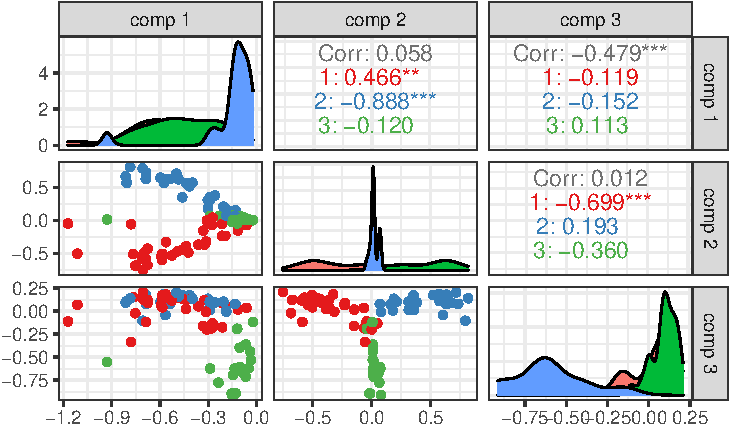
\includegraphics{draft_files/figure-latex/ukfaculty-ase-1} 

}

\caption{A three-dimensional ASE of the UK faculty network using the three most positive eigenvalues and their corresponding eigenvectors. The vertices are labeled by the school to which each faculty member belongs.}\label{fig:ukfaculty-ase}
\end{figure}

\end{example}

The PABM is also a Bernoulli random graph, so it is also a GRDPG.
The latent vectors of the PABM when viewed as a GRDPG form \(K\) \(K\)-dimensional subspaces, which makes for an elegant parallel between the nested forms of the block models and the nested structures of the GRDPGs: The SBM consists of \(K\) zero-dimensional subspaces, and DCBM consists of \(K\) one-dimensional subspaces.
We explore this connection further the next section (section \ref{sec:pabm-grdpg}).

\newpage

\hypertarget{sec:pabm-grdpg}{%
\section{Popularity Adjusted Block Models are Generalized Random Dot Product Graphs}\label{sec:pabm-grdpg}}

In this section, we connect the PABM to the GRDPG and exploit that connection to develop algorithms for community detection and parameter estimation.
In order to make the explicit connection between the PABM and the GRDPG, we make use of an alternative but equivalent definition of the PABM which parameterizes the model in terms of popularity vectors, which are collections of popularity parameters.

\begin{remark}
\label{rem:pabm_view2}
In a PABM, each vertex $i$ has $K$ popularity parameters $\lambda_{i1}, \dots, \lambda_{iK}$, that describe its affinity toward each of the $K$ communities. 
Another view of a PABM is as follows.
Let $\tilde{P}$ be the matrix obtained by permuting the rows and columns of $P$ so that the vertices are reorganized by community memberships $z_i \in \{1,2,\dots,K\}$ in increasing order. 
Denote by $\tilde{P}^{(k \ell)}$ the $n_k \times n_{\ell}$ submatrix of $\tilde{P}$ corresponding to the edge probabilities between vertices in communities $k$ and $\ell$. 
Note that $\tilde{P}^{(k \ell)} = (\tilde{P}^{(\ell k)})^\top$. 
Next let $\lambda^{(k \ell)} = \{\lambda_{i \ell} \colon z_i = k\} \in \mathbb{R}^{n_k}$; the elements of $\lambda^{(k \ell)}$ are the affinity parameters toward the $\ell$th community of all vertices in the $k^{th}$ community. 
Define $\lambda^{(\ell k)}$ analogously. 
Then each block $\tilde{P}^{(k \ell)}$ can be written as the outer product of two vectors:
\begin{equation} \label{eq:pabm}
\tilde{P}^{(k \ell)} = \rho_n \lambda^{(k \ell)} (\lambda^{(\ell k)})^{\top}.
\end{equation} 

We will henceforth use the notation \(A \sim \PABM(\{\lambda^{(k \ell)}\}_K, \rho_n)\) to denote a random adjacency matrix \(A\) drawn from a PABM with $K$ communities, popularity parameters \(\{\lambda^{(k \ell)}\}\) and sparsity parameter $\rho_n$.
\end{remark}

\hypertarget{the-geometry-of-pabms}{%
\subsection{The Geometry of PABMs}\label{the-geometry-of-pabms}}

In section \ref{sec:sbm-dcbm-grdpg}, we showed how the SBM and DCBM are special cases of the GRDPG in which the latent vectors form a very particular geometry.
Similarly, we now show the special geometry of the PABM when viewed as a GRDPG.
For ease of exposition, and without loss of generality, we drop the dependency on the sparsity parameter \(\rho_n\) and assume \(\rho_n \equiv 1\) throughout this subsection.

\begin{theorem}[The latent configuration of the PABM]
\label{thm:pabm-grdpg}
Let $A \sim \mathrm{PABM}(\{\lambda^{(k \ell)}\}_K)$ be an instance of a
PABM with $K \geq 1$ blocks and latent vectors $\{\lambda^{(k \ell)}
\colon 1 \leq k \leq K, 1 \leq \ell \leq K\}$. 
Then there exists a block diagonal matrix
$X \in \mathbb{R}^{n \times K^2}$ defined by $\{\lambda^{(k \ell)}\}$ and a 
$K^2 \times K^2$ {\em fixed} orthonormal matrix $U$ such 
that $A \sim \mathrm{GRDPG}_{K (K+1) / 2, K (K-1) /
2}(\tilde{\Pi}XU)$. Here $\tilde{\Pi}$ is the permutation matrix
such that $P = \tilde{\Pi} \tilde{P} \tilde{\Pi}^{\top}$ where the
rows and columns of $\tilde{P}$ are arranged according to increasing values of the
community labels (see remark~\ref{rem:pabm_view2}). 
\end{theorem}

\begin{proof}
We will prove this theorem in two parts. First, for demonstration
purposes, we focus on the case when $K = 2$ to build intuition. 
The general case of $K \geq 2$ is presented later.  

For the $K = 2$ case, the proof is straightforward. We will first work with
the matrix $\tilde{P}$. Note that $\tilde{P}$ has the form

$$\tilde{P} = \begin{bmatrix} P^{(11)} & P^{(12)} \\ P^{(21)} &
P^{(22)} \end{bmatrix} = \begin{bmatrix} \lambda^{(11)} (\lambda^{(11)})^\top & \lambda^{(12)} (\lambda^{(21)})^\top \\
\lambda^{(21)} (\lambda^{(12)})^\top & \lambda^{(22)}
(\lambda^{(22)})^\top \end{bmatrix}.$$
Now let
$$X = \begin{bmatrix}
\lambda^{(11)} & \lambda^{(12)} & 0 & 0 \\
0 & 0 & \lambda^{(21)} & \lambda^{(22)}
\end{bmatrix} \quad \text{and} \quad
U = \begin{bmatrix} 1 & 0 & 0 & 0 \\
0 & 0 & 1 / \sqrt{2} & 1 / \sqrt{2} \\
0 & 0 & 1 / \sqrt{2} & - 1 / \sqrt{2} \\
0 & 1 & 0 & 0 \end{bmatrix}.$$
Then by straightforward matrix multiplication, we obtain 
$$X U I_{3, 1} U^\top X^\top =
\begin{bmatrix}
\lambda^{(11)} (\lambda^{(11)})^\top & \lambda^{(12)} (\lambda^{(21)})^\top \\
\lambda^{(21)} (\lambda^{(12)})^\top & \lambda^{(22)} (\lambda^{(22)})^\top
\end{bmatrix} = \tilde{P}$$
and hence $\tilde{P}$ also corresponds to the edge probability matrix of GRDPG
with latent vectors described by $X U$. As $P = \tilde{\Pi} \tilde{P}
\tilde{\Pi}^{\top}$ we conclude that $P$ has latent vectors described
by $\tilde{\Pi} X U$. 

It is nevertheless instructive to look at a few intermediate steps. 
More specifically, the product $U I_{3, 1} U^\top$ 
yields a permutation matrix $\Pi$ with fixed points at positions $1$ and $4$ 
and a cycle of order 2 swapping positions $2$ and $3$, i.e., 
$$\Pi = U I_{3, 1} U^\top = \begin{bmatrix} 1 & 0 & 0 & 0 \\
0 & 0 & 1 & 0 \\
0 & 1 & 0 & 0 \\
0 & 0 & 0 & 1
\end{bmatrix}.$$
Furthermore, as $U$ is orthonormal and $I_{3, 1}$ is diagonal, 
$U I_{3, 1} U^\top$ is also an eigendecomposition of $\Pi$ where the fixed
points of $\Pi$ are mapped to the eigenvectors $e_1$ and $e_4$
while the cycles of order two are mapped to the eigenvectors  
$\tfrac{1}{\sqrt{2}}(e_{2} + e_3)$ and $\tfrac{1}{\sqrt{2}}(e_{2} -
e_3)$; here $e_i$ denote the $i^\mathrm{th}$ basis vector in $\mathbb{R}^{4}$. 
Thus, another way of decomposing the edge probability matrix is
$\tilde{P} = X \Pi X^\top$ where the rows of $X$ lie in the union of
two 2-dimensional orthogonal subspaces and $\Pi$ is a permutation matrix. 

For the general case, we can extend $\tilde{P} = X \Pi X^\top$ to larger $K$. 
For a more concrete example of this, refer to Example~1. 
We once again consider $\tilde{P}$ as defined in
remark~\ref{rem:pabm_view2}.  
We first define the following matrices

\begin{gather}
\label{eq:xy}
\Lambda^{(k)} = \begin{bmatrix} \lambda^{(k1)} \mid \cdots \mid \lambda^{(kK)} \end{bmatrix}
\in \mathbb{R}^{n_k \times K}, \quad
X = \mathrm{blockdiag}(\Lambda^{(1)}, \dots, \Lambda^{(K)}) \in
\mathbb{R}^{n \times K^2}, \\
L^{(k)} = \mathrm{blockdiag}(\lambda^{(1k)}, \dots, \lambda^{(Kk)}) \in
\mathbb{R}^{n \times K}, \quad
Y = \begin{bmatrix} L^{(1)} \mid \cdots \mid L^{(K)} \end{bmatrix} \in
\mathbb{R}^{n \times K^2}.
\end{gather}

It is then straightforward to verify that

\begin{gather*}
XY^{\top} = \mathrm{blockdiag}(\Lambda^{(1)}, \dots,
\Lambda^{(K)}) \begin{bmatrix} L_1^{\top} \\ \vdots \\
L_{K}^{\top} \end{bmatrix} = \begin{bmatrix} \Lambda^{(1)}
(L^{(1)})^{\top} \\ \vdots \\
\Lambda^{(K)} (L^{(K)})^{\top} \end{bmatrix}, \\
\Lambda^{(k)} (L^{(k)})^{\top} = \begin{bmatrix} \lambda^{(k1)}
(\lambda^{(1k)})^{\top} \mid \dots \mid \lambda^{(kK)}
(\lambda^{(Kk)})^{\top} \end{bmatrix} = \begin{bmatrix} P^{(k1)}
\mid P^{(k2)} \mid \dots \mid P^{(kK)} \end{bmatrix}.
\end{gather*}
We therefore have $\tilde{P} = X Y^\top$. 
Similar to the $K = 2$ case, we also have $Y = X \Pi$ for some permutation matrix
$\Pi$ and hence $\tilde{P} = X \Pi X^\top$.
The permutation described by $\Pi$ now has $K$ fixed points, which correspond to
$K$ eigenvalues equal to $1$ with corresponding eigenvectors $e_k$ where
$k = r (K + 1) + 1$ for $0 \leq r \leq K - 1$. It also has
$\tbinom{K}{2}$ cycles of order $2$. Each cycle corresponds to
a pair of eigenvalues $\{-1,+1\}$ and a pair of eigenvectors
$\{(e_s + e_t)/\sqrt{2},(e_s - e_t)/ \sqrt{2}\}$. 

Let $p = K (K + 1) / 2$ and $q = K (K - 1) / 2$. 
We therefore have
\begin{equation} \label{eq:permutation}
\Pi = U I_{p,q} U^\top
\end{equation}
where $U$ is a $K^2 \times K^2$ orthogonal matrix and hence
\begin{equation} \label{eq:pabm-grdpg}
\tilde{P} = X U I_{p, q} (X U)^\top.
\end{equation}
In summary we can describe the PABM with $K$ communities as a GRDPG with latent
positions $\tilde{\Pi} X U$ and known signature $(p,q) = \bigl( \tfrac{1}{2} K (K + 1) ,
\tfrac{1}{2} K (K - 1)\bigr)$.
\end{proof}

\begin{example} Let $A$ be a $3$ blocks PABM with latent vectors $\{\lambda^{(k \ell)} \colon 1 \leq k \leq 3, 1 \leq \ell \leq 3\}$. 
Using the same notation as in theorem~\ref{thm:pabm-grdpg}, we can define
\begin{gather*}
X = \begin{bmatrix}
\lambda^{(11)} & \lambda^{(12)} & \lambda^{(13)} & 0 & 0 & 0 & 0 & 0 & 0 \\
0 & 0 & 0 & \lambda^{(21)} & \lambda^{(22)} & \lambda^{(23)} & 0 & 0 & 0 \\
0 & 0 & 0 & 0 & 0 & 0 & \lambda^{(31)} & \lambda^{(32)} & \lambda^{(33)}
\end{bmatrix}, \\
Y = \begin{bmatrix}
\lambda^{(11)} & 0 & 0 & \lambda^{(12)} & 0 & 0 & \lambda^{(13)} & 0 & 0 \\
0 & \lambda^{(21)} & 0 & 0 & \lambda^{(22)} & 0 & 0 & \lambda^{(23)} & 0 \\
0 & 0 & \lambda^{(31)} & 0 & 0 & \lambda^{(32)} & 0 & 0 & \lambda^{(33)}
\end{bmatrix}.
\end{gather*}
Then $Y = X \Pi$ and $\tilde{P} = X Y^{\top}$ where $\Pi$ is a $9 \times 9$ 
permutation matrix of the form
$$\Pi = 
\Bigl[e_1 \mid e_4 \mid e_7 \mid e_2 \mid e_5 \mid e_8 \mid e_3
\mid e_6 \mid e_9 \Bigr].$$
where $e_i$ denotes the $i^{th}$ basis vector in $\mathbb{R}^{9}$. 
The matrix $\Pi$ corresponds to a permutation of $\{1,2,\dots,9\}$ with the following decomposition.
\begin{enumerate}
\item Positions 1, 5, 9 are fixed.
\item There are three cycles of length 2, namely $(2, 4)$, $(3, 7)$, and $(6, 8)$.
\end{enumerate}
We can thus write $\Pi$ as $\Pi = U I_{6, 3} U^\top$ where the first three columns of $U$ consist of $e_1$, $e_5$, and $e_9$ corresponding to the fixed points, the next three columns are the eigenvectors $(e_k + e_{\ell}) / \sqrt{2}$, and the last three columns are the eigenvectors $(e_k - e_{\ell}) / \sqrt{2}$ for $(k, \ell) \in \{(2,4),(3,7),(6,8)\}$.

The matrix $\tilde{P}$ is then the edge probabilities matrix for a 
Generalized Random Dot Product Graph whose latent positions 
are the rows of the matrix
$$XU = \begin{bmatrix}
\lambda^{(11)} & 0 & 0 &
\frac{\lambda^{(12)}}{\sqrt{2}} & \frac{\lambda^{(13)}}{\sqrt{2}} & 0 &
\frac{\lambda^{(12)}}{\sqrt{2}} & \frac{\lambda^{(13)}}{\sqrt{2}} & 0 \\
0 & \lambda^{(22)} & 0 &
\frac{\lambda^{(21)}}{\sqrt{2}} & 0 & \frac{\lambda^{(23)}}{\sqrt{2}} &
-\frac{\lambda^{(21)}}{\sqrt{2}} & 0 & \frac{\lambda^{(23)}}{\sqrt{2}} \\
0 & 0 & \lambda^{(33)} &
0 & \frac{\lambda^{(31)}}{\sqrt{2}} & \frac{\lambda^{(32)}}{\sqrt{2}} &
0 & -\frac{\lambda^{(31)}}{\sqrt{2}} & -\frac{\lambda^{(32)}}{\sqrt{2}}
\end{bmatrix}$$
and the latent positions for $P$ is a permutation of the rows of
$XU$. 
\end{example}

\hypertarget{algorithms}{%
\subsection{Algorithms}\label{algorithms}}

Two inference objectives arise from the PABM:

\begin{enumerate}
\def\labelenumi{\arabic{enumi}.}
\tightlist
\item
Community membership identification (up to permutation).
\item
Parameter estimation (estimating $\lambda_{ik}$'s).
\end{enumerate}

In our methods, the data that are observed for estimation is the adjacency matrix, \(A \sim \PABM(\{\lambda^{(k \ell)}\}_K, \rho_n)\), along with an assumed number of communities, \(K\).
To motivate our methods, we first consider community detection and parameter estimation in the case where we know the edge probability matrix \(P\) beforehand, noting that community memberships and popularity parameters are not immediately discernible from \(P\) itself.
After establishing methods for community detection and parameter estimation from \(P\), we use the consistency property of the ASE \citep{doi:10.1080/01621459.2012.699795,rubindelanchy2017statistical} to demonstrate that the same methods work for \(A\) almost surely as \(n \to \infty\).

\hypertarget{previous-work}{%
\subsubsection{Previous Work}\label{previous-work}}

\citet{307cbeb9b1be48299388437423d94bf1}
used Modularity Maximization (MM) and the Extreme Points (EP)
algorithm \citep{le2016} for community detection and parameter
estimation. They were able to show that as the sample size increases,
the \emph{proportion} of misclassified community labels (up to permutation)
goes to 0.

\cite{noroozi2019estimation} used Sparse Subspace Clustering (SSC)
\citep{5206547} for community detection in the PABM.
The SSC algorithm can be described as follows:
Given \(X \in \mathbb{R}^{n \times d}\) with vectors
\(x_i^\top \in \mathbb{R}^d\) as rows of \(X\), the optimization problem
\(c_i = \mathop{\mathrm{arg\,min}}_{c} \|c\|_1\) subject to \(x_i = X^\top c\) and
\(c^{(i)} = 0\), where \(c^{(i)}\) is the \(i^{th}\) entry of \(c\), is solved for each \(i \in [n]\).
The solutions are collected into matrix
\(C = \bigl[ c_1 \mid \cdots \mid c_n \bigr]^\top\) to
construct an affinity matrix \(B = |C| + |C^\top|\). If each \(x_i\) lies
exactly on one of \(K\) subspaces, \(B\) describes an undirected graph
consisting of \emph{at least} \(K\) disjoint subgraphs, i.e., \(B_{ij} = 0\) if \(x_i, x_j\) lie on different subspaces.
The intuition here is that vectors that lie on the same subspace can be described as linear combinations of each other, assuming the number of vectors in the subspace is greater than the dimensionality of the subspace.
Then once sparsity is enforced, for each \(c_i\), its \(j^{th}\) element \(c_i^{(j)}\) is zero if \(x_j\) belongs to a subspace that doesn't contain \(x_i\), resulting in \(B_{ij} = 0\).
If \(X\) instead represents points near \(K\) subspaces with some noise,
then this property may only hold approximately and a final graph partitioning step may be required
(e.g., edge thresholding or spectral clustering).

In practice, due to presence of noise, SSC is often done by solving the LASSO problems
\begin{equation} 
\label{eq:ssc}
c_i = \mathop{\mathrm{arg\,min}}_c \frac{1}{2} \|x_i - X_{-i}^\top c\|^2_2 + \vartheta \|c\|_1
\end{equation}
for some sparsity parameter \(\vartheta > 0\).
The \(c_i\) vectors are then collected into \(C\) and \(B\) as before.

\begin{definition}[Subspace Detection Property]
\label{def:subspace_detection}
Let $X = \bigl[ x_1 \mid \cdots \mid x_n \bigr]^\top$ be noisy points sampled from $K$ subspaces, i.e., $x_i = y_i + z_i$ where the $y_i$ belongs to the union of $K$ subspaces and the $z_i$ are noise vectors. 
Let $\vartheta \geq 0$ be given and let $C$ and $B$ be constructed from the solutions of LASSO problems as described in equation~\eqref{eq:ssc} with this given choice of $\vartheta$. 
Then $X$ is said to satisfy the subspace detection property with sparsity parameter $\vartheta$ if each column of $C$ has nonzero $\ell_2$ norm and $B_{ij} = 0$ whenever $y_i$ and $y_j$ are from different subspaces.
\end{definition}

\begin{remark}
\label{rem:sdp}
One common approach to show that SSC works for a noisy sample $X$ is to show that $X$ satisfies the subspace detection property for some choice of $\vartheta$; 
recall that $\vartheta$ is the sparsity parameter for
the LASSO problems in equation~\eqref{eq:ssc}. However, this is not sufficient to
guarantee that SSC perfectly recovers the underlying subspaces.
More specifically, if $X$ satisfies the 
subspace detection property, 
then $B$ describes a graph with {\em at least} $K$ disconnected subgraphs, 
with the ideal case being that there are exactly $K$ subgraphs 
which map onto each subspace. 
Nevertheless it is also possible that the $K$ subspaces are represented by
$K' > K$
multiple disconnected subgraphs and we cannot, at least without a subsequent
post-processing step, recover the $K$ subspaces directly from $B$;
see \citet{sdp_sufficiency} and \citet{liu_ssc}
for further discussions. Therefore in practice $B$ is usually treated as an
affinity matrix and, as we allude to earlier, 
the rows of $B$ are partitioned using some
clustering algorithm to obtain the final clustering. 
\end{remark}

Theorem \ref{thm:pabm-grdpg} suggests that SSC is appropriate for community
detection for the PABM, provided that we observe the edge probabilities
matrix \(P\). More precisely, given the matrix \(\tilde{P}\) obtained by
permuting the rows and columns of \(P\) as described in
remark \ref{rem:pabm_view2} we can recover \(XU\) up
to some non-identifiability indefinite orthogonal transformation \(Q\).
Then using results from \citet{soltanolkotabi2012}, it can be easily shown
that the subspace detection property holds for \(XU\). Indeed, the columns
of \(XU\) from different communities correspond to mutually
orthogonal subspaces. This then implies that the
subspace detection property also holds for \(XUQ\) for all invertible
transformation \(Q\) and hence the subspace detection property also holds for
\(\tilde{\Pi} X U Q\) for any \(n \times n\) permutation matrix \(\tilde{\Pi}\).

However, because we do not observe \(P\) but rather only the noisy
adjacency matrix \(A \sim \BG(P)\), the natural approach then is
to perform SSC on the rows of the spectral embedding of \(A\),
since the embedding of \(P\) consists of \(K\) subspaces (theore \ref{thm:pabm-grdpg}),
and so the embedding of \(A\) will lie approximately on the \(K\) subspaces.
We will show in theorem \ref{thm:ssc} that, with probability converging to
one as \(n \rightarrow \infty\), the rows of the ASE of \(A\) also
satisfy the subspace detection property.
Theorem \ref{thm:ssc} builds upon existing work by
\citet{rubindelanchy2017statistical} who describe the convergence
behavior of the ASE of \(A\) to that of \(\tilde{\Pi} XU\), and
\citet{jmlr-v28-wang13} who show the necessary conditions for the
subspace detection property to hold in noisy cases where the points lie
near subspaces. Finally we emphasize that while
\citet{noroozi2019estimation} also considered the use of SSC for
community recovery in PABM, they instead applied SSC to the rows of
\(A\) itself, foregoing
the embedding step altogether. It is however much harder to show that
the rows of \(A\) satisfy the subspace detection property and thus, to
the best of our knowledge, there is currently no consistency result
regarding the application of SSC to the rows of \(A\).

\hypertarget{algorithms-for-community-detection}{%
\subsubsection{Algorithms for Community Detection}\label{algorithms-for-community-detection}}

We previously stated in theorem \ref{thm:pabm-grdpg} one possible set of latent positions that result in
the edge probability matrix of a PABM, namely
\(P = \tilde{\Pi} (XU) I_{p, q} (XU)^\top \tilde{\Pi}^{\top}\) where \(X\) is block diagonal and
\(\tilde{\Pi}\) is a permutation matrix.\\
Furthermore, the explicit form of \(XU\) represents points in \(\mathbb{R}^{K^2}\)
such that points within each community lie on \(K\)-dimensional
orthogonal subspaces, i.e.~\(\langle U^{\top} x_i, U^{\top} x_j \rangle = 0\) whenever \(i\) and \(j\) are in different communities.
Thus if we have (or can estimate) \(XU\) directly, then both the community
detection and parameter identification problem are trivial because \(U\)
is orthonormal and fixed for each value of \(K\).
However, direct
identification or estimation of \(XU\) is possibly difficult
due to the non-identifiability of \(XU\) (see remark \ref{rem:non_identifiable})
when we are given only \(P\).
More specifically, suppose we find a matrix \(Y \in \mathbb{R}^{n \times K^2}\)
such that \(P = Y I_{p, q} Y^\top\). Then it is generally the case that
\(Y = \tilde{\Pi} XU Q\) for some indefinite orthogonal matrix
\(Q \in \mathbb{O}(p,q)\).
However since \(Q\) is not necessarily an
orthogonal matrix and hence, if \(y_i\) denote the \(i^{th}\) row of \(Y\),
then \(\langle U^{\top} x_i, U^{\top} x_j \rangle \neq \langle y_i, y_j \rangle\).
This prevents us from transferring the orthogonality property of
\(XU\) directly to \(Y\).

Nevertheless by using the special geometric structure of \(X\) we can circumvent the
non-identifiability of \(Y\) and \(XU\) by using instead the rows of the
matrix \(V\) of eigenvectors (corresponding to the non-zero eigenvalues) of \(P\). In particular \(V\) is identifiable
up to orthogonal transformations and furthermore, due to the block
diagonal structure of \(X\), the rows of \(V\) also lie on \(K\) distinct orthogonal
subspaces and hence \(v_i^{\top} v_j = 0\) whenever \(z_i \not = z_j\).

\begin{theorem}
\label{thm:osc-p}
Let $P = V D V^\top$ be the spectral decomposition 
of the edge probability matrix. 
Let $B = n V V^\top$. 
Assume $\lambda_{i z_i} > 0$ for each $i \in [n]$, 
i.e., each vertex's popularity parameter to its own community is nonzero. 
Then $B_{ij} = 0$ if and only if 
vertices $i$ and $j$ are in different communities.
\end{theorem}

\begin{proof}
We first show that $V V^\top =
\tilde{\Pi} X (X^\top X)^{-1} X^\top \tilde{\Pi}^{\top} $ where $X$ is 
defined as in equation~\eqref{eq:xy}. Indeed, by Theorem 2, 
\(P = \tilde{\Pi} X U I_{p, q} U^\top X^\top \tilde{\Pi}\) for $p = K(K+1)/2$ and $q = K(K-1)/2$. 
The eigendecomposition \(P = V D V^\top\) also yields $P = V
|D|^{1/2} I_{p, q} |D|^{1/2} V^\top$ where \(|\cdot|^{1/2}\) is
applied entry-wise. Now let $Y = \tilde{\Pi} XU$ and $\tilde{Y} = V|D|^{1/2}$; note that
$Y$ and $\tilde{Y}$ both have full column ranks. 
Because $P = Y I_{p,q} Y^{\top} = \tilde{Y} I_{p,q} \tilde{Y}^{\top}$, we have
$$Y = \tilde{Y} I_{p,q} \tilde{Y}^{\top} Y (Y^{\top} Y)^{-1} I_{p,q}.$$
Let $Q = I_{p,q} \tilde{Y}^{\top} Y (Y^{\top} Y)^{-1} I_{p,q}$ and note that
$Y = \tilde{Y} Q$. We then have
\begin{equation*}
\begin{split}
Q^{\top} I_{p,q} Q &= I_{p,q} (Y^{\top} Y)^{-1} Y^{\top} \tilde{Y} I_{p,q}
I_{p,q} I_{p,q} \tilde{Y}^{\top} Y (Y^{\top} Y)^{-1} I_{p,q} \\ 
&= I_{p,q} (Y^{\top} Y)^{-1} Y^{\top} Y I_{p,q}
Y^{\top} Y (Y^{\top} Y)^{-1} I_{p,q} =  I_{p,q}
\end{split}
\end{equation*}
and hence $Q$ is an indefinite orthogonal matrix. 

Let $R = U Q |D|^{-1/2}$ and note that $V = \tilde{\Pi} XR$. Because $R$ is
invertible, we can write
$$\tilde{\Pi} X (X^{\top} X)^{-1} X^{\top} \tilde{\Pi}^{\top} =
\tilde{\Pi} X R (R^{\top} X^{\top} X R)^{-1}
R^{\top} X^{\top} \tilde{\Pi}^{\top}.$$ 
Furthermore, as $V$ has orthonormal columns, $R^{\top} X^{\top} X R =
V^{\top} \tilde{\Pi} \tilde{\Pi}^{\top} V = V^{\top} V = I$. We thus conclude
$$\tilde{\Pi} X (X^{\top} X)^{-1} X^{\top} \tilde{\Pi}^{\top} = V (V^{\top} V)^{-1} V^{\top} = V V^{\top}$$
as desired.

To complete the proof of theorem \ref{thm:osc-p}, recall that \(X\) 
is block diagonal with each block corresponding to one community, 
and hence \(X (X^\top X)^{-1} X^\top\) is also a
block diagonal matrix with each block corresponding to a community. 
As $B = n VV^{\top} = n \tilde{\Pi} X (X^\top X)^{-1} X^\top \tilde{\Pi}^{\top}$, 
we conclude that $B_{ij} = 0$ 
whenever vertices $i$ and $j$ belong to different communities.  
\end{proof}

Theorem \ref{thm:osc-p} provides perfect community detection from \(P\).
More specifically, let \(|B|\) be the affinity matrix for graph \(G'\),
where \(|\cdot|\) is applied entry-wise. Then
\(G'\) consists of exactly \(K\) disjoint subgraphs,
as \(G'\) has no edges between communities.
All that is left to identify the communities is
to assign each subgraph a distinct community label.
In practice, we do not observe \(P\) and instead only observe the noisy
\(A \sim \BG(P)\). A natural approach is then to use
the affinity matrix \(\hat{B} = n \hat{V} \hat{V}^{\top}\) where
\(\hat{V}\) is the matrix of eigenvectors (corresponding to the largest
eigenvalues in modulus) of \(A\). The resulting procedure, named
Orthogonal Spectral Clustering, is presented in
algorithm \ref{alg:osc}.
The following result leverages existing theoretical properties
of ASE for estimating of latent positions in a GRDPG \citep{rubindelanchy2017statistical} to show that
\(\hat{B}\) converges almost surely to \(B\); in particular
\(\hat{B}_{ij} \stackrel{a.s.}{\to} 0\)
for each pair \((i, j)\) in different communities.

\begin{algorithm}[tp]
\label{alg:osc}
\setstretch{1.5}
\DontPrintSemicolon
\SetAlgoLined
\KwData{Adjacency matrix $A$, number of communities $K$}
\KwResult{Community assignments $z_1, ..., z_n \in \{1, ..., K\}$}
Compute the eigenvectors of $A$ that correspond to the $K (K+1) / 2$ most
positive eigenvalues and $K (K-1) / 2$ most negative eigenvalues. Construct
$V$ using these eigenvectors as its columns.\;
Compute $B = |n V V^\top|$, applying $|\cdot|$ entry-wise.\;
Construct graph $G$ using $B$ as its similarity matrix.\;
Partition $G$ into $K$ disconnected subgraphs
(e.g., using edge thresholding or spectral clustering).\;
Map each partition to the community labels $1, ..., K$.\;
\caption{Orthogonal Spectral Clustering.}
\end{algorithm}

\begin{theorem}
\label{thm:osc}
Assume the setting of theorem \ref{thm:osc-p}. 
Let $\hat{B}$ with entries $\hat{B}_{ij}$ be the affinity matrix
obtained from OSC as described in algorithm~\ref{alg:osc}. 
Then for $n \rho_n = \omega(\log^{4}{n})$, we have
\begin{equation} 
\label{eq:osc}
\max_{i, j} |\hat{B}_{ij} - B_{ij}| = O\Big( \frac{\log n}{\sqrt{n \rho_n}} \Big)
\end{equation}
with high probability. In particular 
$\hat{B}_{ij} -B_{ij} \overset{\mathrm{a.s.}}{\rightarrow} 0$ 
where the convergence is
uniform over all $i,j$. Hence for all pairs $(i,j)$ in different
communities we have 
$\hat{B}_{ij} \overset{\mathrm{a.s.}}{\rightarrow} 0$, 
while for all pairs $(i, j)$ in the same community, 
$\liminf_{n \to \infty} |\hat{B}_{ij}| > 0$ almost surely. 
\end{theorem}

Theorem \ref{thm:osc} guarantees that for any \(\epsilon > 0\),
the number of edges of \(\hat{B}\) between vertices of different communities that are larger than \(\epsilon\) converges to zero with probability converging to one as \(n\) increases.
We can always find an \(\epsilon > 0\) such that \(\hat{B}_{ij} > \epsilon\) with probability converging to one as \(n\) increases.
Thus, by using \(\hat{B}\), we can perfectly recover all the latent community assignments \(z_1, z_2, \dots, z_n\), i.e., the number of misclustered vertices is zero asymptotically almost surely.
We note that theorem \ref{thm:osc} is stronger than existing results in the literature;
in particular theorem 1 of \citet{307cbeb9b1be48299388437423d94bf1} (the paper that
originally introduces the PABM model) only guarantees that the \emph{proportion} of misclustered vertices converges to \(0\) as \(n \rightarrow \infty\).
Furthermore theorem 1 of \citet{307cbeb9b1be48299388437423d94bf1} also requires the sparsity parameter \(\rho_n\) to satisfies \(n \rho_n^2 = \omega(\log^2{n})\) which is a considerably stronger assumption than the assumption \(n \rho_n =\omega(\log^{4}{n})\) used in theorem \ref{thm:osc}.
Indeed, \(n\rho_n^2 = \omega(\log^{2}{n})\) implies \(n \rho_n = \omega(n^{1/2})\).
We emphasize that the assumption \(n \rho_n = \omega(\log^{c}{n})\) for some constant \(c > 1\) is commonly used in the context of graph estimation using spectral methods.

Theorems \ref{thm:pabm-grdpg}, \ref{thm:osc-p}, and \ref{thm:osc} also provide
a natural path toward using SSC for community detection.
In particular we established in theorem \ref{thm:pabm-grdpg} that an ASE of the edge
probability matrix \(P\) can be constructed from a latent vector configuration
consisting of orthogonal subspaces. Theorem \ref{thm:osc-p} shows how
this property can also be recovered from the eigenvectors of \(P\).
Then theorem \ref{thm:osc} shows that, by replacing \(P\) with \(A\), the
rows of \(\hat{V}\) also lie on asymptotically orthogonal subspaces.
Motivated by theorem \ref{thm:osc}, theorem \ref{thm:ssc} below
shows that the subspace detection property also holds for the rows of
\(\sqrt{n} \hat{V}\).

\begin{algorithm}[t]
\label{alg:ssc}
\setstretch{1.5}
\DontPrintSemicolon
\SetAlgoLined
\caption{Sparse Subspace Clustering using LASSO.}
\KwData{Adjacency matrix $A$, number of communities $K$,
hyperparameter $\lambda$}
\KwResult{Community assignments $z_1, ..., z_n \in \{1, ..., K\}$}
Find $V$, the matrix of eigenvectors of $A$
corresponding to the $K (K + 1) / 2$ most positive
and the $K (K - 1) / 2$ most negative eigenvalues.\;
Normalize $V \leftarrow \sqrt{n} V$.\;
\For {$i = 1, ..., n$} {
Assign $v_i^\top$ as the $i^{th}$ row of $V$.
Assign $V_{-i} = \bigl[
v_1 \mid \cdots \mid v_{i-1} \mid v_{i+1} \mid \cdots \mid v_n \bigr]^\top$.\;
Solve the LASSO problem
$c_i = \arg\min_{\beta}
\frac{1}{2} \|v_i - V_{-i} \beta\|_2^2 + \lambda \|\beta\|_1$.\;
Assign $\tilde{c}_i = (c_i^{(1)}, \dots, c_i^{(i-1)}, 0, c_i^{(i)}, \dots, c_i^{(n-1)})^\top$ such that the superscript is the index of
$\tilde{c}_i$.\;
}
Assign
$C = \bigr[ \tilde{c}_1 \mid \cdots \mid \tilde{c}_n \bigr]$.\;
Compute the affinity matrix $B = |C| + |C^\top|$.\;
Construct graph $G$ using $B$ as its similarity matrix.\;
Partition $G$ into $K$ disconnected subgraphs (e.g., using edge
thresholding or spectral clustering).\;
Map each partition to the community labels $1, ..., K$.
\end{algorithm}

\begin{theorem}
\label{thm:ssc}
Let $P$ describe the edge probability matrix of the PABM with $n$ vertices, and let $A \sim \Bernoulli(P)$. 
Let $\hat{V}$ be the matrix of eigenvectors of $A$ corresponding to the $K^2$ largest eigenvalues in modulus. 
Then for any $\epsilon > 0$, there exists a choice of $\vartheta > 0$ and $N \in \mathbb{N}$ such that for all $n \geq N$, $\sqrt{n} \hat{V}$ obeys the subspace detection property with probability at least $1 - \epsilon$.  
\end{theorem}

\hypertarget{algorithm-for-parameter-estimation}{%
\subsubsection{Algorithm for Parameter Estimation}\label{algorithm-for-parameter-estimation}}

For ease of exposition we now assume in this subsection that the edge probability matrix \(P\) for the PABM had been arranged so that the rows and columns are organized by community so that \(\tilde{P} = P\) (see remark \ref{rem:pabm_view2}).
Then the \(k\ell\)\textsuperscript{th} block is an outer product of two vectors, i.e., \(P^{(k \ell)} = \lambda^{(k \ell)} (\lambda^{(\ell k)})^\top\).
Therefore, given \(P^{(k \ell)}\), \(\lambda^{(k \ell)}\) and \(\lambda^{(\ell k)}\) are solvable up to multiplicative constant using singular value decomposition.
More specifically, let \(P^{(k \ell)} = (\sigma^{(k \ell)})^2 u^{(k \ell)} (v^{(k \ell)})^\top\) be the singular value decomposition of \(P^{(k \ell)}\) where \(u^{(k \ell)} \in \mathbb{R}^{n_k}\) and \(v^{(k \ell)} \in \mathbb{R}^{n_\ell}\) are vectors and \(\sigma^{(k \ell)}\) is a scalar.
Then \(\rho_n^{1/2} \lambda^{(k \ell)} = s_1 u^{(k \ell)}\) and \(\rho_n^{1/2} \lambda^{(\ell k)} = s_2 v^{(k \ell)}\) for unidentifiable \(s_1 s_2 = (\sigma^{(k \ell)})^2\).
Because each \(\lambda^{(k \ell)}\) is not strictly identifiable, we instead estimate each \(\tilde{\lambda}^{(k \ell)} = \sigma^{(k \ell)} u^{(k \ell)}\).
Given the adjacency matrix \(A\) instead of edge probability matrix \(P\), we can simply use plug-in estimators by taking the SVD of each \(A^{(k \ell)}\) to obtain \(\hat{\lambda}^{(k \ell)} = \hat{\sigma}^{(k \ell)} \hat{u}^{(k \ell)}\) using the largest singular value of \(A\) and its corresponding singular vectors.

\begin{algorithm}[tp]
\label{alg:param_est}
\DontPrintSemicolon
\SetAlgoLined
\setstretch{1.5}
\caption{PABM parameter estimation.}
\KwData{Adjacency matrix $A$, community assignments $1, ..., K$}
\KwResult{PABM parameter estimates $\{\hat{\lambda}^{(k \ell)}\}_K$.}
Arrange the rows and columns of $A$ by community such that each 
$A^{(k \ell)}$ block consists of estimated edge probabilities between 
communities $k$ and $l$.\;
\For {$k, \ell = 1, ..., K$, $k \leq \ell$} {
Compute $A^{(k \ell)} = U \Sigma V^\top$, the SVD of the $k\ell^{th}$ block.\;
Assign $u^{(k \ell)}$ and $v^{(k \ell)}$ as the first columns of $U$ and $V$. 
Assign $(\sigma^{(k \ell)})^2 \leftarrow \Sigma_{11}$.\;
Assign $\hat{\lambda}^{(k \ell)} \leftarrow \pm \sigma^{(k \ell)} u^{(k \ell)}$ and $\hat{\lambda}^{(\ell k)} \leftarrow \pm \sigma^{(k \ell)} v^{(k \ell)}$.
}
\end{algorithm}

\begin{theorem}
\label{thm:param-est}
Let each $\tilde{\lambda}^{(k \ell)}$ be the popularity vector derived from its corresponding $P^{(k \ell)}$ and let $\hat{\lambda}^{(k \ell)}$ be its estimate obtained from $A^{(k \ell)}$ using algorithm~\ref{alg:param_est}.
Then if $n \rho_n = \omega( \log^{4}{n})$,
\begin{equation} 
\label{eq:param-est}
\max_{k, \ell \in \{1, ..., K\}} 
\|\hat{\lambda}^{(k \ell)} - \tilde{\lambda}^{(k \ell)}\|_{\infty} = 
O\bigg(\frac{\log n_k}{\sqrt{n_k}} \bigg)
\end{equation}
with high probability. 
Here $\|\cdot\|_{\infty}$ denotes the $\ell_\infty$ norm of a vector. Let $\hat{\Lambda}$ be the matrix
$$\hat{\Lambda} = \begin{bmatrix} \hat{\lambda}^{(11)} &
\hat{\lambda}^{(12)} & \cdots & \hat{\lambda}^{(1 K)} \\
\hat{\lambda}^{(21)} &
\hat{\lambda}^{(22)} & \cdots & \hat{\lambda}^{(2 K)} \\
\vdots & \vdots & \cdots & \vdots \\
\hat{\lambda}^{(K1)} &
\hat{\lambda}^{(K2)} & \cdots & \hat{\lambda}^{(K K)} 
\end{bmatrix}$$
and let $\hat{P} = \hat{X} U I_{p,q} U^\top \hat{X}^{\top}$, where $\hat{X}$ is defined from $\hat{\Lambda}$ and $U$ is defined from $K$ as in theorem~\ref{thm:pabm-grdpg}. 
Equation~\eqref{eq:param-est} then implies
\begin{equation}
\label{eq:conv_prob}
\frac{1}{n} \|\rho_n^{-1} \hat{P} - \rho_n^{-1} P\|_{F} = O((n
\rho_n)^{-1/2}), \quad \max_{ij} |\rho_n^{-1} \hat{P}_{ij} -
\rho_n^{-1} P_{ij}| = O((n \rho_n)^{-1/2})
\end{equation}
with high probability. 
\end{theorem}

Equation \eqref{eq:param-est} guarantees that \(n^{-1/2} \|\rho_n^{-1/2} \hat{\Lambda} - \Lambda\|_{F} = O((n \rho_n)^{-1/2})\).
Equation \eqref{eq:conv_prob} then guarantees that the mean square error for \(\rho_n^{-1} (\hat{P} - P)\) converges to \(0\) almost surely and furthermore the entries of \(\rho_n^{-1} \hat{P}\) converge uniformly to the entries of \(\rho_n^{-1} P\);
recall that \(\rho_n^{-1} P_{ij} = \lambda_{iz_j} \lambda_{j z_i}\).
We note that these results are stronger than existing results in \citet{307cbeb9b1be48299388437423d94bf1};
for example theorem 2 in \citet{307cbeb9b1be48299388437423d94bf1} only guarantees
\(n^{-1/2} \|\rho_n^{-1/2} \hat{\Lambda} - \Lambda\|_{F} = o(1)\) as \(n \rightarrow \infty\).

\hypertarget{simulation-study}{%
\subsection{Simulation Study}\label{simulation-study}}

For each simulation, community labels are drawn from a multinomial
distribution, the popularity vectors \(\{\lambda^{(k \ell)}\}_K\) are drawn
from two types of joint distributions depending on whether \(k = \ell\) or \(k \not = \ell\). The edge probability matrix \(P\) is constructed using the popularity
vectors and finally the adjacency matrix \(A\)
is drawn \(A \sim \mathrm{Bernoulli}(P)\). OSC (algorithm \ref{alg:osc}) is then used for community detection, and this
method is compared against (1) SSC using the spectral embedding \(\hat{V}\)
(algorithm \ref{alg:ssc}), (2) SSC using the rows of the
observed adjacency matrix \(A\) as is done in \citet{noroozi2019estimation}
and (3) modularity maximization (MM) as is done in
\citet{307cbeb9b1be48299388437423d94bf1}. We denote the two SSC
implementations using the rows of \(A\) and using the spectral embedding
of \(A\) as SSC-A and SSC-ASE, respectively.
The parameters \(\vartheta\)
that controls the sparsity for SSC-A and SSC-ASE were chosen via a preliminary cross-validation experiment.
In practice, \(\vartheta\) that guarantee SDP (if it is possible for the particular simulated data) often result in more than \(K\) disconnected subgraphs, so a smaller \(\vartheta\) that does not guarantee SDP was chosen,
and the final clustering step of SSC-A and SSC-ASE was done
by fitting a Gaussian mixture model to the normalized Laplacian
eigenmap embeddings \citep{belkin03:_laplac} of the affinity matrix \(B\).
We also estimate the latent popularity vectors \(\{\lambda^{(k \ell)}\}\)
by assuming that the true community labels are known and then apply
algorithm \ref{alg:param_est}, and we compare this estimation method against an
MLE-based estimator as described in \citet{noroozi2019estimation} and
\citet{307cbeb9b1be48299388437423d94bf1}.

Modularity maximization is NP-hard, so
\citet{307cbeb9b1be48299388437423d94bf1} used the extreme points
(EP) algorithm (\cite{le2016}) as a greedy
relaxation of the optimization problem; the EP algorithm has a running
time of \(O(n^{K-1})\) where \(n\) is the number of vertices in the graph
and \(K\) is the number of communities.
For these simulations we instead replace the EP algorithm with the
Louvain algorithm for modularity maximization,
as the implementation of the EP algorithm in
\citet{307cbeb9b1be48299388437423d94bf1} is too computationally expensive for \(K > 2\). For \(K = 2\), it
was verified that the Louvain algorithm produces comparable results
to EP-MM.

For comparing methods, we define the community detection error as:
\[L_c(\hat{\sigma}, \sigma; V) = \min_\pi \sum_i I(\pi \circ \hat{\sigma}(v_i) = \sigma(v_i))\]
where \(\sigma(v_i)\) is the true community label of vertex \(v_i\), \(\hat{\sigma}(v_i)\) is the predicted label of \(v_i\), and \(\pi\) is a permutation operator.
This is effectively the ``misclustering count'' of clustering function \(\hat{\sigma}\).

For parameter estimation, because the popularity parameters \(\{\lambda_{ik}\}\) are unidentifiable, we instead estimate the edge probabilities \(P_{ij} = \lambda_{i z_j} \lambda_{j z_i}\) via the quantities \(\hat{P}_{ij} = \hat{\lambda}_{iz_j} \hat{\lambda}_{jz_i}\).
The parameter estimation error is then given by the normalized Frobenius norm of \(P\) divided by the number of vertices, i.e.,
\[\mathrm{RMSE}(\hat{P}, P) = \frac{1}{n} \|\hat{P} - P\|_F.\]

We also note that unlike the MLE-based method \citep{307cbeb9b1be48299388437423d94bf1}, the ASE method in algorithm \ref{alg:param_est} can be trivially modified so as to not require the community labels if we are only interested in estimating \(P\).
More specifically we first compute the ASE \(\hat{Z}\) of \(A\) (see definition \ref{def:ase}) and then compute \(\hat{P} = \hat{Z} I_{p,q} \hat{Z}^{\top}\).
The resulting estimate \(\hat{P}\) will have the same convergence rate as that given in equation (\ref{eq:conv_prob}).

\hypertarget{sec:balanced-communities}{%
\subsubsection{Balanced Communities}\label{sec:balanced-communities}}

In each simulation, community labels \(z_1, ..., z_n\) were drawn from a
multinomial distribution with mixture parameters
\(\{\alpha_1, ..., \alpha_K\}\), then \(\{\lambda^{(k \ell)}\}_K\) according
to the drawn community labels, \(P\) was constructed using the drawn
\(\{\lambda^{(k \ell)}\}_K\), and \(A\) was drawn from \(P\).

For these examples, we set the following parameters:

\begin{itemize}
\tightlist
\item
Number of vertices \(n = 128, 256, 512, 1024, 2048, 4096\)
\item
Number of underlying communities \(K = 2, 3, 4\)
\item
Mixture parameters \(\alpha_k = 1 / K\) for \(k = 1, ..., K\), (i.e.,
each community label has an equal probability of being drawn)
\item
Community labels
\(z_k \stackrel{\text{iid}}{\sim} \Multinomial(\alpha_1, ..., \alpha_K)\)
\item
Within-group popularities
\(\lambda^{(kk)} \stackrel{\text{iid}}{\sim} \Betadist(2, 1)\)
\item
Between-group popularities
\(\lambda^{(k \ell)} \stackrel{\text{iid}}{\sim} \Betadist(1, 2)\) for
\(k \neq \ell\)
\end{itemize}

Fifty simulations were performed for each combination of \(n\) and \(K\).
The results for community recovery and parameter estimations are presented in figures \ref{fig:clust_err_ct_sim} and \ref{fig:p_block_est}, respectively.

Figure \ref{fig:clust_err_ct_sim} shows that OSC recovers the community
perfectly as \(n\) increases, i.e., the number of mislabeled vertices
goes to \(0\).
The performance of SSC-ASE is comparable to OSC for \(K \geq 3\) but is noticeably worse when \(K = 2\).
Similarly, SSC on both the embedding and on the adjacency matrix produces similar trends for \(K > 2\).
The difference in performance between SSC-A and SSC-ASE for \(K = 2\) can be attributed to the final spectral clustering step of the affinity matrix. While the subspace detection property is guaranteed for large \(n\), in our simulations, setting the
sparsity parameter \(\vartheta\) to the required value usually resulted
in more than \(K\) disconnected subgraphs in the affinity matrix
\(\hat{B}\).
We instead chose a smaller sparsity parameter,
necessitating a final clustering step.
A GMM was fit to the normalized Laplacian eigenmap of \(\hat{B}\),
but visual inspection suggests that the communities are not
distributed as a mixture of Gaussians in the eigenmap.
A different choice of mixture distribution may result in better performance.

\begin{figure}[tp]
{\centering \includegraphics{/home/johnkoo/dev/pabm-grdpg/summary_files/figure-latex/clust_err_ct_sim-1}
}
\caption{Median and IQR of community detection error. Communities are approximately balanced. Simulations were repeated 50 times for each sample size.}
\label{fig:clust_err_ct_sim}
\end{figure}

Given ground truth community labels, figure \ref{fig:p_block_est} shows
that algorithm \ref{alg:param_est} and the MLE-based
plug-in estimators perform comparably, with root mean square
error decaying at rate approximately \(n^{-1/2}\) as \(n\) increases.

\begin{figure}[tp]
{\centering \includegraphics{/home/johnkoo/dev/pabm-grdpg/summary_files/figure-latex/lambda_est_p-1}}
\caption{Median and IQR RMSE for edge probability matrices
reconstructed from the outputs of algorithm~\ref{alg:param_est}
(red) compared against outputs of an MLE-based method (blue) proposed in \citet{307cbeb9b1be48299388437423d94bf1}.
Simulations were repeated 50 times for each sample size. Communities were drawn to be approximately balanced.}
\label{fig:p_block_est}
\end{figure}

\hypertarget{sec:imbalanced-communities}{%
\subsubsection{Imbalanced Communities}\label{sec:imbalanced-communities}}

Simulations performed in this section are the same as those in the
previous section with the exception of the mixture parameters
\(\{\alpha_1, ..., \alpha_K\}\) used to draw community labels from the
multinomial distribution. For these examples, we set the following
parameters:

\begin{itemize}
\tightlist
\item
Number of vertices \(n = 128, 256, 512, 1024, 2048, 4096\)
\item
Number of underlying communities \(K = 2, 3, 4\)
\item
Mixture parameters \(\alpha_k = \frac{k^{-1}}{\sum_{\ell=1}^K \ell^{-1}}\)
for \(k = 1, ..., K\)
\item
Community labels
\(z_k \stackrel{\text{iid}}{\sim} \Multinomial(\alpha_1, ..., \alpha_K)\)
\item
Within-group popularities
\(\lambda^{(kk)} \stackrel{\text{iid}}{\sim} \Betadist(2, 1)\)
\item
Between-group popularities
\(\lambda^{(k \ell)} \stackrel{\text{iid}}{\sim} \Betadist(1, 2)\) for
\(k \neq \ell\)
\end{itemize}

Fifty simulations were performed for each combination of \(n\) and \(K\).
The results for community recovery and parameter estimations are presented in figures \ref{fig:clust_err_ct_sim_imba} and \ref{fig:lambda_est_p_imba}, respectively.

From figure \ref{fig:clust_err_ct_sim_imba} we once again see that the
number of mislabeled vertices trending to \(0\) for OSC.
The performance of SSC-ASE is comparable to that of OSC for \(K > 2\) but is worse when \(K = 2\).
Figure \ref{fig:lambda_est_p_imba} indicates that the parameter estimation error also decays at rate \(n^{-1/2}\) similar to that in the balanced communities setting.

\begin{figure}[H]
{\centering \includegraphics{/home/johnkoo/dev/pabm-grdpg/summary_files/figure-latex/clust_err_ct_sim_imba-1}
}
\caption{Median and IQR of community detection error. Communities are imbalanced. 
Simulations were repeated 50 times for each sample size.}\label{fig:clust_err_ct_sim_imba}
\end{figure}

\begin{figure}[H]
{\centering \includegraphics{/home/johnkoo/dev/pabm-grdpg/summary_files/figure-latex/lambda_est_p_imba-1}
}
\caption{Median and IQR RMSE of edge probabilities derived from the
outputs of Algorithm \ref{alg:param_est} (red) compared against an
MLE-based method (blue) described in
\cite{307cbeb9b1be48299388437423d94bf1}.
Simulations were repeated 50 times for each sample size. Communities were drawn to be imbalanced.}
\label{fig:lambda_est_p_imba}
\end{figure}

\hypertarget{sec:disassortative-models}{%
\subsubsection{Disassortative Models}\label{sec:disassortative-models}}

\citet{rubindelanchy2017statistical} demonstrated the power of applying GRDPG-based approaches to disassortative block models.
Likewise, demonstrate that GRDPG-based algorithms OSC and SSC-ASE perform well on disassortative PABMs.
Simulations performed in this section are the same as those in section \ref{sec:balanced-communities} with the exception of the distributions from which within and between-group popularity parameters are drawn.
Here, we draw these parameters such that the expected value is \(1/3\) for the within-group popularity parameters and \(2/3\) for the between-group popularity parameters:

\begin{itemize}
\tightlist
\item
Number of vertices \(n = 128, 256, 512, 1024, 2048, 4096\)
\item
Number of underlying communities \(K = 2, 3, 4\)
\item
Mixture parameters \(\alpha_k = \frac{k^{-1}}{\sum_{\ell=1}^K \ell^{-1}}\)
for \(k = 1, ..., K\)
\item
Community labels
\(z_k \stackrel{\text{iid}}{\sim} \Multinomial(\alpha_1, ..., \alpha_K)\)
\item
Within-group popularities
\(\lambda^{(kk)} \stackrel{\text{iid}}{\sim} \Betadist(1, 2)\)
\item
Between-group popularities
\(\lambda^{(k \ell)} \stackrel{\text{iid}}{\sim} \Betadist(2, 1)\) for
\(k \neq \ell\)
\end{itemize}

OSC, SSC-ASE, and SSC-A perform similarly on disassortative PABMs compared to the simulations in sections \ref{sec:balanced-communities} and \ref{sec:imbalanced-communities}
(figures \ref{fig:clust_k_disassortative} and \ref{fig:lambda_est_disassortative}).

\begin{figure}[H]
{\centering \includegraphics{/home/johnkoo/dev/pabm-grdpg/summary_files/figure-latex/clust_err_k_disassortative}
}
\caption{Median and IQR of community detection error. 
Communities are approximately balanced. 
Edge probabilities were drawn to be disassortative. 
Simulations were repeated 50 times for each sample size.}
\label{fig:clust_k_disassortative}
\end{figure}

\begin{figure}[H]
{\centering \includegraphics{/home/johnkoo/dev/pabm-grdpg/summary_files/figure-latex/lambda_est_disassortative}
}
\caption{Median and IQR RMSE of edge probabilities derived from the
outputs of algorithm \ref{alg:param_est} (red) compared against an
MLE-based method (blue) described in
\cite{307cbeb9b1be48299388437423d94bf1}.
Simulations were repeated 50 times for each sample size. 
Communities were drawn to be approximately balanced.
Edge probabilities were drawn to be disassortative.}
\label{fig:lambda_est_disassortative}
\end{figure}

\begin{remark}
While we call the models in this section ``disassortative'', it is our view that the assortative/disassortative distinction is not applicable to PABMs due to its flexibility. 
Unlike the SBM and DCBM, in the PABM, each vertex is free to have a higher affinity to its own community or to other communities, independent of each other. 
In other words, within the same community, $v_i$ may have a larger popularity parameter to its own community whereas $v_j$ may have a larger popularity parameter to a different community. 
Furthermore, when viewed as GRDPGs, the assortativity or disassortativity of SBMs and DCBMs affects whether $P$ is positive semidefinite, which affects ASE-based approaches to analyzing the graph \citep{rubindelanchy2017statistical}, 
but in the full rank PABM, $P$ is never positive semidefinite and will always have $K (K + 1) / 2$ positive eigenvalues and $K (K - 1) / 2$ negative eigenvalues. 
\end{remark}

\hypertarget{applications}{%
\subsection{Applications}\label{applications}}

In the first example, we applied OSC (algorithm \ref{alg:osc}) to the Leeds Butterfly
dataset \citep{Wang_2018} consisting of visual similarity measurements
among 832 butterflies across 10 species. The graph was modified to match
the example from \citet{noroozi2019estimation}: Only the \(K=4\) most
frequent species were considered, and the similarities were discretized
to \(\{0, 1\}\) via thresholding.
Figure \ref{fig:butterfly} shows a sorted adjacency matrix sorted by the resultant clustering.

Comparing against the ground truth species labels, \citet{noroozi2019estimation}
report that SSC on the adjacency matrix achieves an adjusted Rand index of 73\% in their implementation, whereas OSC achieves 92\% and SSC on the ASE achieves 96\%.

\begin{figure}[H]

{\centering \includegraphics{/home/johnkoo/dev/pabm-grdpg/summary_files/figure-latex/butterfly-1}

}

\caption{Adjacency matrix of the Leeds Butterfly dataset 
after sorting by the clustering outputted by OSC.}\label{fig:butterfly}
\end{figure}

In the second example (figure \ref{fig:mp} and table \ref{tab:unnamed-chunk-6}), we applied OSC to the British MPs Twitter network
\citep{greene2013producing}, the Political Blogs network
\citep{10.1145/1134271.1134277}, and the DBLP network
\citep{NIPS2009_3855, 10.1007/978-3-642-15880-3_42}.
For this data analysis, we subsetted the data as described in
\citet{307cbeb9b1be48299388437423d94bf1} for their analysis of the
same networks. Our methods slightly underperformed compared to modularity
maximization, although performance is comparable.
The run time of OSC is however much smaller than that of modularity maximization.

\begin{figure}[H]
{\centering \includegraphics{/home/johnkoo/dev/pabm-grdpg/summary_files/figure-latex/mp-1}
}
\caption{Adjacency matrices of (from left to right) the British MPs, Political Blogs, and DBLP networks after sorting by the clustering outputted by OSC.}\label{fig:mp}
\end{figure}

\begin{table}[H]
\centering
\begin{tabular}[t]{l|r|r|r}
\hline
Network & MM & SSC-ASE & OSC\\
\hline
British MPs & 0.003 & 0.012 & 0.006\\
\hline
Political Blogs & 0.050 & 0.187 & 0.062\\
\hline
DBLP & 0.028 & 0.072 & 0.059\\
\hline
\end{tabular}
\caption{\label{tab:unnamed-chunk-6}Community detection error rates on the British MPs Twitter, Political Blogs, and DBLP networks using modularity maximization, sparse subspace clustering, and OSC.}
\end{table}

In the third example (figure \ref{fig:households-figure} and
table \ref{tab:households-table}),
we analyzed the Karantaka villages data studied by
\citet{DVN/U3BIHX_2013}. We chose the \texttt{visitgo}
networks from villages 12, 31, and 46 at the household level.
In these networks, each node is a household and each edge is
an interaction between members of pairs of households.
The label of interest is the religious affiliation.
The networks were truncated to religions ``1'' and ``2'',
and vertices of degree 0 were removed.
The villages were chosen based on there being an adequate number of nodes
between households within each religion.

\begin{figure}[H]
{\centering \includegraphics{/home/johnkoo/dev/pabm-grdpg/summary_files/figure-latex/unnamed-chunk-7-1}
}
\caption{Adjacency matrix of the Karnataka villages data, arranged by the clustering produced by OSC (left). The villages studied here are, from left to right, 12, 31, and 46.}\label{fig:households-figure}
\end{figure}

\begin{table}[H]
\centering
\begin{tabular}[t]{l|r|r|r}
\hline
Network & MM & SSC-ASE & OSC\\
\hline
Village 12 & 0.270 & 0.291 & 0.227\\
\hline
Village 31 & 0.125 & 0.059 & 0.051\\
\hline
Village 46 & 0.052 & 0.069 & 0.056\\
\hline
\end{tabular}
\caption{\label{tab:households-table}Community detection error rates for identifying household religion.}
\end{table}

\newpage

\hypertarget{sec:mbm}{%
\section{Generalized Random Dot Product Graphs with Nonlinear Community Structure}\label{sec:mbm}}

\hypertarget{community-detection-as-clustering-in-the-latent-space}{%
\subsection{Community Detection as Clustering in the Latent Space}\label{community-detection-as-clustering-in-the-latent-space}}

As established in section \ref{sec:grdpg}, all Bernoulli random graphs are generalized random dot product graphs.
Whether this is useful for community detection in block models depends entirely on the configuration of the latent vectors.
In the case of the \(\ER\) model, SBM, DCBM, and PABM, each community forms a linear structure, i.e., a subspace, and this rigid structure can be exploited for community detection.
In this section, we explore GRDPGs with community-wise parameterized nonlinear latent structures.

To motivate this model, consider a generalization of the \(\ER\) model in which each edge probability isn't constant but comes from a simple distribution.
As with all Bernoulli random graphs, this is also a GRDPG, but by using a specific type of distribution, it is possible to construct specific latent structures on which the latent vectors lie.
Or, in reverse, by constructing specific latent structures, the edge probabilities of the Bernoulli random graph follow specific distributions.

\begin{example}
In the $\ER$ model, the edge probability matrix has a fixed value $P_{ij} \equiv p \in [0, 1]$. 
This corresponds to a one-dimensional RDPG with a latent structure $X = \Big[ \sqrt{p},  \cdots, \sqrt{p} \Big]^\top$. 
In another view, the RDPG with latent structure $X = \Big[ \sqrt{p}, \cdots, \sqrt{p} \Big]^\top$ induces an $\ER$ model in which the edge probabilities have a fixed value. 

Suppose that we have RDPG in which the latent space is in $\mathbb{R}^2$ and the latent vectors are drawn uniformly from the quarter unit circle defined by $g(t) = \Big[ \cos \frac{\pi}{2} t, \sin \frac{\pi}{2} t \Big]^\top$ for $t \in [0, 1]$. 
Then it can be shown that instead of a fixed $P_{ij} = p$, this RDPG induces a model in which the edge probabilities follow a distribution with density $f(p) = \frac{2}{\pi - 2} \Big( \frac{1}{1 - p^2} - 1 \Big)$. 
\end{example}

By changing the latent structure from a point mass to a curve, we are able to come up with more flexible Bernoulli random graph models in which the edge probabilities follow more general probability distributions.
Community structure can then be added by sampling latent vectors from multiple curves.
The goal of this section is to explore GRDPGs with such structures and develop algorithms for community detection and parameter estimation.

\hypertarget{the-manifold-block-model}{%
\subsection{The Manifold Block Model}\label{the-manifold-block-model}}

We begin by defining the model:

\begin{definition}[Manifold block model]
\label{def:mbm}
Let $p, q \geq 0$, $d = p + q \geq 1$, $1 \leq r < d$, $K \geq 2$, and $n > K$ be integers. 
Define manifolds $\mathcal{M}_1, ..., \mathcal{M}_K \in \mathcal{X}$ for $\mathcal{X} = \{x, y \in \mathbb{R}^d : x^\top I_{p,q} y \in [0, 1]\}$ each by continuous function $g_k : [0, 1]^r \to \mathcal{X}$. 
Define probability distributions $F_1, ..., F_K$ each with support $[0, 1]^r$. 
Then the following mixture model is a {\em manifold block model}.

\begin{enumerate}
\item Draw labels $z_1, ..., z_n \iid \Multinomial(\alpha_1, ..., \alpha_K)$.
\item Draw latent vectors by first taking each $t_i \indep F_{z_i}$ and then computing each $x_i = g_{z_i}(t_i)$. 
\item Compile the latent vectors into data matrix $X = \Big[ x_1 \mid \cdots \mid x_n \Big]^\top$ and define the adjacency matrix as $A \sim \GRDPG_{p,q}(X; \rho_n)$. 
\end{enumerate}
\end{definition}

Definition \ref{def:mbm} describes the most general version of the manifold block model (MBM).
Some plausible constraints may be to fix one distribution for each underlying distribution \(F_{z_i} \equiv F\) or to restrict the manifolds to be one-dimensional, i.e., \(r \equiv 1\).
We use these constraints to construct the following example:

\begin{example}
\label{ex:separated-curves}
Define two one-dimensional manifolds in $\mathbb{R}^2$ by $f_1(t) = \Big[ \cos(\frac{\pi}{3} t), \sin(\frac{\pi}{3} t) \Big]^\top$ and $f_2(t) = \Big[ 1 - \cos(\frac{\pi}{3} t), 1 - \sin(\frac{\pi}{3} t) \Big]^\top$.
Draw $t_1, ..., t_n \iid \Uniform(0, 1)$ and $z_1, ..., z_n \iid \Multinomial(\frac{1}{2}, \frac{1}{2})$, and compute latent vectors $x_i = f_{z_i}(t_i)$, which are collected in data matrix $X = \Big[ x_1 \mid \cdots \mid x_n \Big]^\top$. 
Finally, let $A \sim \RDPG(X)$. Figure~\ref{fig:two-curves} shows the latent configuration drawn from this latent distribution, a random dot product graph drawn from the latent configuration, and the ASE of the graph. 
Although the community structure is not obvious from the graph, the embedding shows a clear separation between the two communities. 

\begin{figure}[H]

{\centering 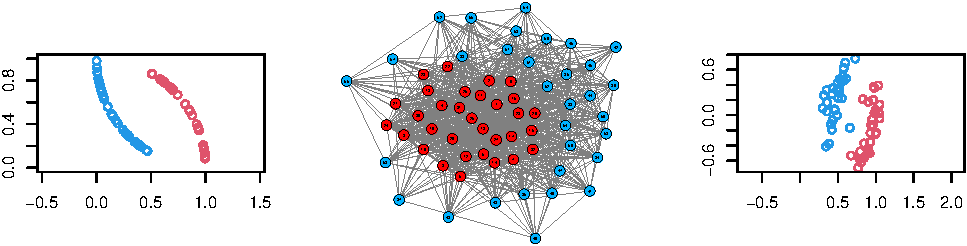
\includegraphics{draft_files/figure-latex/two-curves-1} 

}

\caption{Manifold block model from two disjoint curves. The latent configuration is on the left, a random dot product graph drawn from the latent configuration is on the middle, and the ASE is on the right.}\label{fig:two-curves}
\end{figure}
\end{example}

In the case of the SBM, a GRDPG-motivated community detection algorithm is to construct the ASE of the graph and then apply a point cloud based clustering algorithm such as \(K\)-means or GMM on the embedding.
We saw that in the case of the DCBM and PABM, because the latent structures are not based on point masses, while the ASE does reveal the communities, the final clustering step requires other clustering algorithms that are tailored to the latent community structure.
Likewise, in the following sections, we develop algorithms specific to the structure of the MBM, one in the case of disjoint manifolds (section \ref{sec:nonintersect}) and one in the general case in which the latent manifolds can intersect (section \ref{sec:intersect}).
We also derive theoretical consistency properties for both settings.

\hypertarget{previous-work-1}{%
\subsubsection{Previous Work}\label{previous-work-1}}

Manifolds have been observed in the ASEs of real observed graphs when they are studied as GRDPGs.
The \emph{Drosophila} connectome graph \citep{Eichler141762} displays community-wise linear and quadratic structures in the ASE.
\citet{https://doi.org/10.48550/arxiv.1705.03297} used GMMs on the ASE for community detection and found that the curve-like structures in the ASE were incompatible with centroid-based clustering methods.
\citet{SannaPassino2022} used Gaussian Processes to estimate curves, which resulted in better empirical fits.
\citet{athreya2020estimation} considered GRDPGs in which the vertices lie on curves or manifolds, but their focus was largely on estimating distributions on the manifolds rather than the manifolds themselves.

Outside of random graph inference, there is a larger body of work on fitting parametric curves to vectors in \(\mathbb{R}^d\) and identifying vectors belonging to different manifolds in \(\mathbb{R}^d\).

\hypertarget{sec:nonintersect}{%
\subsection{Algorithm for Nonintersecting Manifolds}\label{sec:nonintersect}}

In this section, we consider the following setting: Suppose that each community \(C_k\) is represented by a closed manifold \(\mathcal{M}_k\) in the latent space of a RDPG or GRDPG.
Define \(\delta = \min\limits_{k \neq \ell} \min\limits_{x \in \mathcal{M}_k, y \in \mathcal{M}_\ell} \|x - y\|\), the minimum distance between two manifolds.
Furthermore, assume that \(\delta > 0\), i.e., the manifolds do not intersect.

In the original latent space, it is possible to construct for each manifold \(\mathcal{M}_k\) a connected \(\eta_k\)-neighborhood graph for some \(\eta_k > 0\).
If the subsample of vectors on each manifold is sufficiently dense such that \(\max_k \eta_k = \eta < \delta\), then an \(\eta\)-neighborhood graph on the entire sample results in a graph with \(K\) disconnected subgraphs that map onto each manifold exactly.
This is equivalent to applying single linkage clustering on the ASE and cutting the dendrogram at \(K\) clusters (see algorithm \ref{alg:ase-singlelink}).
The remainder of this section explores under which conditions these criteria are met for the latent configuration, in which the latent vectors lie exactly on manifolds, as well as for the ASE of the GRDPG sampled from these latent configurations, in which the vectors lie approximately on manifolds with some noise that approaches zero asymptotically.

\begin{algorithm}[h]
\label{alg:ase-singlelink}
\DontPrintSemicolon
\SetAlgoLined
\setstretch{1.5}
\KwData{Adjacency matrix $A$, number of communities $K$, embedding dimensions $(p, q)$.}
\KwResult{Community assignments $z_1, ..., z_n \in \{1, ..., K\}$.}
Compute $\hat{X}$, the ASE of $A$ using the $p$ most positive and $q$ most negative eigenvalues and their corresponding eigenvectors.\;
Apply single linkage clustering with $K$ communities on $\hat{X}$.\;
\caption{ASE clustering for nonintersecting communities.}
\end{algorithm}

\begin{theorem}[Community detection for the GRDPG for which the communities come from nonintersecting manifolds]
\label{theorem:nonintersect-grdpg}
Let $x_1, ..., x_n$ be points sampled on $K$ compact, connected manifolds $\mathcal{M}_1, ..., \mathcal{M}_K \subset \mathbb{R}^d$ each with probability measures $F_1, ..., F_K$, and the manifolds are separated by distance at least $\delta = \min\limits_{k \neq \ell} \min\limits_{x_i \in \mathcal{M}_k, x_j \in \mathcal{M}_\ell} \| x_i - x_j \| > 0$. 
Let $X = \Big[ x_1 \mid \cdots \mid x_n \Big]^\top$ and $A \sim \GRDPG_{p,q}(X; \rho_n)$ for some $p, q \in \mathbb{N}_0$ such that $p + q = d$ and sparsity parameter $\rho_n$ that satisfies $n \rho_n = \omega(\log^c n)$ for some $c > 1$. 
Define $A_n(\eta)$ as the event that an $\eta$-neighborhood graph constructed from the ASE of $A$ consists of exactly $K$ disconnected subgraphs that map exactly to each manifold. 
Then for some $C > 0$ and any $\eta \in (0, C \delta)$, $\lim\limits_{n \to \infty} P(A_n(\eta)) = 1$. 
\end{theorem}

If the manifolds are one-dimensional, then a more precise rate of convergence can be derived.

\begin{example}
\label{ex:separated-curves-2}
Refer back to the RDPG in example \ref{ex:separated-curves} in which the latent vectors are drawn uniformly from two nonintersecting curves. 
Figure \ref{fig:two-curves} shows that while the ASE introduces noise to the original latent vectors, there is still sufficient separation between the two communities. 
Applying single-linkage clustering on the ASE results in recovering the original community labels, up to permutation (figure \ref{fig:two-curves-2}). 

\begin{figure}[H]

{\centering 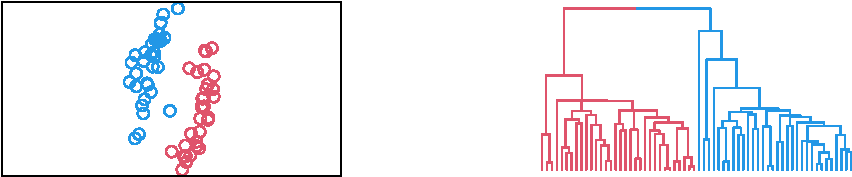
\includegraphics{draft_files/figure-latex/two-curves-2-1} 

}

\caption{Single-linkage clustering applied to the ASE of an MBM with two nonintersecting curves. The ASE is on the left and the dendrogram from single-linkage clustering, colored by the original community labels, is on the right.}\label{fig:two-curves-2}
\end{figure}
\end{example}

\hypertarget{sec:intersect}{%
\subsection{Algorithm for Intersecting Manifolds}\label{sec:intersect}}

The consistency of the ASE provides asymptotic guarantees for perfect community label recovery for the nonintersecting MBM.
This relies on the fact that single-linkage clustering and \(\eta\)-neighborhood clustering graphs result in disconnected components if clusters of points are far away from each other.
However, many graphs do not behave so nicely.
For example, the DCBM and PABM can both be viewed as MBMs in which the latent vectors come from (linear) manifolds that intersect at the origin (see section \ref{sec:sbm-dcbm-grdpg}).
Nonlinear intersecting manifolds have also been observed in ASEs of real graphs \citep{SannaPassino2022, https://doi.org/10.48550/arxiv.1709.05454}.
While the DCBM and PABM cases can be handled by algorithms specific to linear structures such as SSC and OSC, nonlinear intersecting manifolds require a more flexible approach.
For the intersecting case, we restrict the MBM to the case in which each \(F_{z_i}\) is identical and univariate on the unit interval \([0, 1]\).
The full mixture model is described as follows:

\begin{enumerate}
\def\labelenumi{\arabic{enumi}.}
\tightlist
\item
  Draw \(t_1, ..., t_n \iid F\) for probability distribution \(F\) with support \([0, 1]\).
\item
  Draw \(z_1, ..., z_n \iid \Multinomial(\alpha_1, ..., \alpha_K)\), the community labels.
\item
  Let each \(x_i = g_{z_i}(t_i)\) be the latent vector for vertex \(v_i\), and collect the latent vectors into matrix \(X = \Big[ x_1 \mid \cdots \mid x_n \Big]^\top\).
\item
  Draw \(A \sim \GRDPG_{p,q}(X; \rho_n)\).
\end{enumerate}

\begin{example}
\label{ex:intersect-curves}
Suppose we have a two-dimensional RDPG in which latent vectors lie on one of two curves defined by the parameterizations $g_1(t) = \Big[ t^2, 2 t (1-t) \Big]^\top$ and $g_2(t) = \Big[ 2 t (1-t), (1-t)^2 \Big]^\top$. 
This can be described as a two-community MBM in which the manifolds are both one-dimensional. 
For simplicity, we restrict $F_1 = F_2 = \Uniform(0, 1)$. 
$g_1$ and $g_2$ intersect at two points, $t = 0$ and $t = 2/3$, which in the latent space correspond to $(0, 0)$ and $(4/9, 4/9)$. 
Clearly, single-linkage or $\eta$-neighborhood clustering does not work for this setting, both in the original latent space and in the ASE. 
The community structure is also not clear from the adjacency matrix. 
However, there still is a clear pattern in the ASE that reveals the community structure (figure \ref{fig:intersect-curves-example}). 

\begin{figure}[H]

{\centering \includegraphics{draft_files/figure-latex/intersect-curves-example-1} 

}

\caption{Latent vectors on intersecting curves (left), along with an RDPG drawn from this configuration (center) and its ASE (right).}\label{fig:intersect-curves-example}
\end{figure}
\end{example}

In this setting, if we know the labels \(z_1, ..., z_n\), then for each \(k\)\textsuperscript{th} subsample for which \(z_i = k\), we can fit the curve \(\hat{g}_k\) (up to an indefinite orthogonal transformation).
On the other hand, if we know the curves \(g_1, ..., g_K\), then we can assign each embedding vector \(\hat{x}_i\) the predicted label \(\hat{z}_i\) based on which curve it is closest to.
This lends itself to an alternating coordinate descent algorithm in which we alternate between fitting curves and assigning labels at each iteration (algorithm \ref{alg:kcurves}).
We call this algorithm \(K\)-curves clustering.
In this algorithm, the loss function that we wish to minimize is
\begin{equation}
\label{eq:kcurves-loss}
L(z_1, ..., z_n, g_1, ..., g_n; X) = \frac{1}{n} \sum_{k=1}^K \sum_{i: z_i = k} \|x_i - g_k(t_i)\|^2
\end{equation}

\begin{algorithm}[h]
\label{alg:kcurves}
\DontPrintSemicolon
\SetAlgoLined
\setstretch{1.5}
\KwData{Adjacency matrix $A$, number of communities $K$, embedding dimensions $p$, $q$, stopping criterion $\epsilon$}
\KwResult{Community assignments $1, ..., K$, curves $g_1, ..., g_K$}
Compute $X$, the ASE of $A$ using the $p$ most positive and $q$ most negative eigenvalues and their corresponding eigenvectors.\;
Initialize community labels $z_1, ..., z_n$.\;
\Repeat {the change in $\sum_k \sum_{i \in C_k} \|x_i - g_k(t_i)\|^2$ is less than $\epsilon$} {
\For {$k = 1, ..., K$} {
Define $X_k$ as the rows of $X$ for which $z_i = k$.\;
Fit curve $g_k$ and positions $t_{k_i}$ to $X_k$ by minimizing $\sum_{k_i} \|x_{k_i} - g_k(t_{k_i})\|^2$.\;
}
\For {$k = 1, ..., K$} {
Assign $z_i \leftarrow \arg\min_\ell \|x_i - g_\ell(t_i)\|^2$.\;
}
}
\caption{$K$-curves clustering.}
\end{algorithm}

\(K\)-curves clustering either requires knowledge of the functional form of each \(g_k\) or a function that is flexible enough to approximate it.
The choice of \(g_k\) affects the difficulty of the algorithm.
As a balance between flexibility and ease of estimation, we consider the case where each \(g_k\) is a Bezier polynomial of degree \(R\) with coefficients \(p_k\).
Then we have \(g_k(t) = g(t; p_k) = \sum_{r=0}^R p_k^{(r)} \binom{R}{r} (1-t)^{R-r} t^r\).

\begin{example}
\label{ex:intersect-curves-fit}
Figure \ref{fig:intersect-curves-2} shows one result of applying algorithm \ref{alg:kcurves} on example \ref{ex:intersect-curves}. 
In this implementation, $g_1$ and $g_2$ are assumed to be Bezier curves in which $p_1^{(0)} = p_2^{(0)} = \Big[ 0, 0 \Big]^\top$, i.e., the curves meet at the origin. 
Here, an accuracy of 87.5\% is achieved. 

\begin{figure}[H]

{\centering 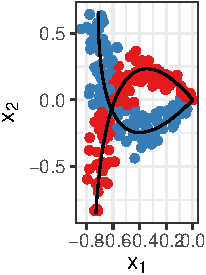
\includegraphics{draft_files/figure-latex/intersect-curves-2-1} 

}

\caption{$K$-curves clustering applied to example \ref{ex:intersect-curves}. The embedding vectors are labeled by predicted community.}\label{fig:intersect-curves-2}
\end{figure}
\end{example}

While example \ref{ex:intersect-curves-fit} achieved high accuracy, algorithm \ref{alg:kcurves} often results in poor performance when it is paired with poor initialization.
In example \ref{ex:intersect-curves-fit}, it just so happened that we randomly chose initial curves that iterated to good fits, but this is not guaranteed.
We also restricted the curves to meet at the origin, which appears to have helped guide the curves to good fits.
In figures \ref{fig:loss} and \ref{fig:init-strategies}, we show the results of various initializations on fitting curves to example \ref{ex:intersect-curves}, such as random initialization and spectral clustering.

\begin{figure}[H]

{\centering \includegraphics{/home/johnkoo/dev/manifold-block-models/draft/draft_files/figure-latex/unnamed-chunk-7-1} 

}

\caption{ASE labeled by estimated community labels for each initialization strategy. Upper right: random initialization assuming intersection at the origin. Upper middle: random initialization without assuming intersection at the origin. Upper right: initialization via spectral clustering assuming intersection at the origin. Lower left: initialization via spectral clustering without assuming intersection at the origin. Lower middle: initialization with ground truth labels, assuming intersection at the origin. Lower right: initialization with ground truth labels, without assuming intersection at the origin.}\label{fig:init-strategies}
\end{figure}

\begin{figure}

{\centering 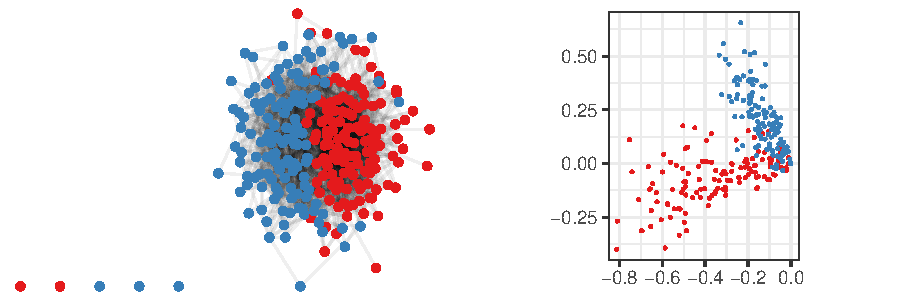
\includegraphics{/home/johnkoo/dev/manifold-block-models/draft/draft_files/figure-latex/unnamed-chunk-6-1} 

}

\caption{Clustering loss vs. iteration for each run of $K$-curve clustering.}\label{fig:loss}
\end{figure}

Alternatively, if we turn this problem into a semi-supervised problem in which we know a few of the community labels, then the convergence of the ASE guarantees high accuracy.

\begin{theorem}
\label{thm:kcurves-semisupervised}
Let $A \sim \MBM(\{\alpha_1, ..., \alpha_K\}, \{F, ..., F\}, \{g_1, ..., g_K\}; \rho_n)$ such that $F$ has support $[0, 1]$, and each $g_k(t) = g(t; p_k)$ is is a Bezier curve of order $R$ that does not self-intersect (for any $s \neq t$, $g_k(s) \neq g_k(t)$). 
Suppose that for each community $k$, we have labels for at least $R + 1$ vertices. 
Then if $n \rho_n = \omega(\log^{4c} n)$, as $n \to \infty$, the estimates outputted by $K$-curves clustering are such that 
$$L(\hat{z}_1, ..., \hat{z}_n, \hat{g}_1, ..., \hat{g}_K; X) \stackrel{p}{\to} 0,$$
where $L$ is the loss function defined in equation (\ref{eq:kcurves-loss}). 
\end{theorem}

\hypertarget{simulation-study-1}{%
\subsection{Simulation Study}\label{simulation-study-1}}

We performed two simulation experiments for algorithm \ref{alg:kcurves}.
In the first simulation setup, we again turn to examples \ref{ex:intersect-curves} and \ref{ex:intersect-curves-fit}.
The setup is as follows:

\begin{enumerate}
\def\labelenumi{\arabic{enumi}.}
\tightlist
\item
  Draw \(z_1, ..., z_n \iid \Multinomial(1/2, 1/2)\).
\item
  Draw \(t_1, ..., t_n \iid \Uniform(0, 1)\).
\item
  Let each \(x_i = g_{z_i}(t_i)\) where \(g_1(t) = \Big[ t^2, 2 t (1-t) \Big]^\top\) and \(g_2(t) = \Big[ 2 t (1-t), (1-t)^2 \Big]^\top\).
  Collect the latent vectors into matrix \(X = \Big[ x_1 \mid \cdots \mid x_n \Big]^\top\).
\item
  Draw \(A \sim \RDPG(X; \rho_n)\) (for these simulations we fix \(\rho_n \equiv 1\)).
\end{enumerate}

For this simulation study, we set \(n = 128, 256, 512, 1024, 2048\), and we start with completely random initialization as well as initializations in which we know 4 or 8 labels from each community.
For each setting, we simulate 50 replicates.
Since the curves meet at the origin, we force the fitted Bezier curves to meet at the origin as well by fixing \(p_1^{(0)} = p_2^{(0)} = (0, 0)\).
Figure \ref{fig:sim-curves} shows the median and interquartile ranges for the error rates for each \(n\) and \emph{a priori} known labels per community.
The simulation results suggest that for sufficient \(n\), we do not benefit from having more known labels, but having a few results in greatly improved performance.

\begin{figure}[H]

{\centering 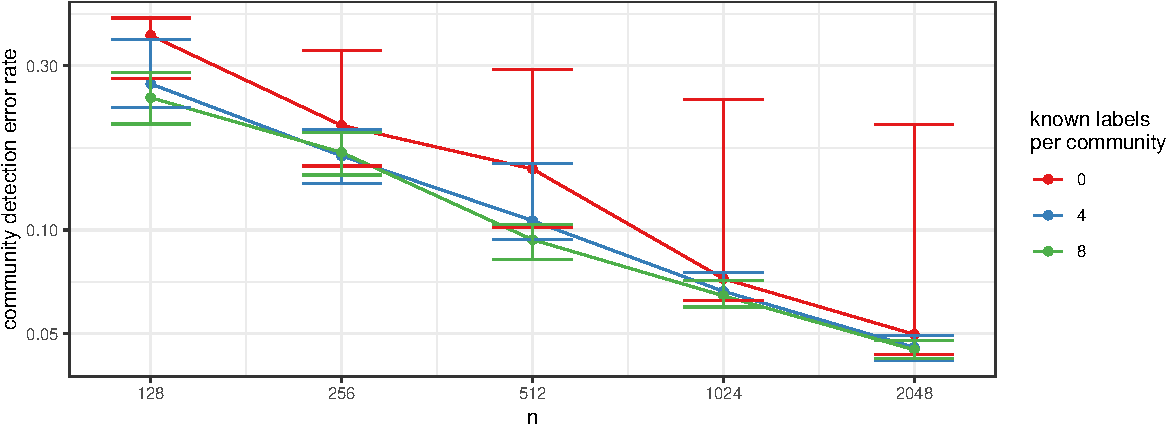
\includegraphics{draft_files/figure-latex/sim-curves-1} 

}

\caption{Median and IQR error rates over 50 replicates in the simulation setting for $K = 2$ curves.}\label{fig:sim-curves}
\end{figure}

We also explored the behavior of random initialization by setting \(n = 512\) and compiling the loss values outputted by \(K\)-curves clustering for each replicate.
Here, we repeated the simulations \(256\) times.
Figure \ref{fig:repeat-losses} suggests that in this particular setting, about half the time, random initialization of \(K\)-curves clustering results in the desired curves, while the rest of the time, \(K\)-curves clustering settled on a local minimum.
Plotting each of the \(256 \times 2\) fitted curves confirms this conclusion (figure \ref{fig:repeat-curves}).

\begin{figure}[H]

{\centering 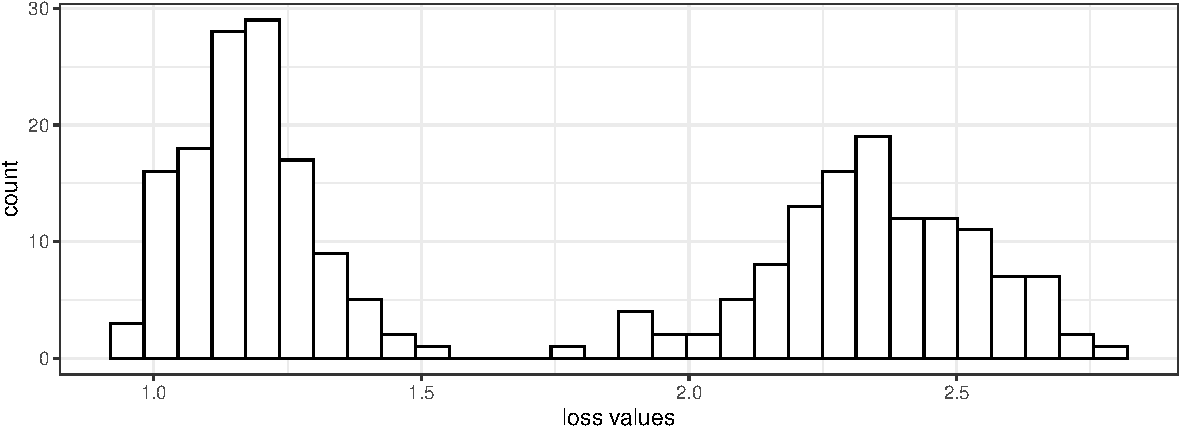
\includegraphics{draft_files/figure-latex/repeat-losses-1} 

}

\caption{Histogram of loss values outputted by $K$-curves clustering over 256 replicates.}\label{fig:repeat-losses}
\end{figure}

\begin{figure}[H]

{\centering 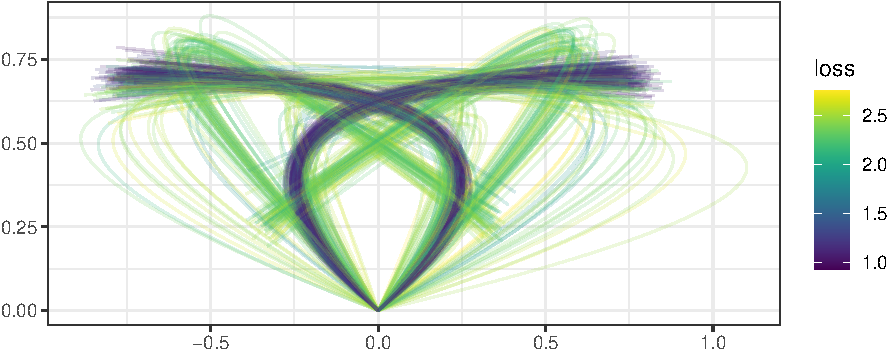
\includegraphics{draft_files/figure-latex/repeat-curves-1} 

}

\caption{Fitted curves over 256 replicates. The curves are colored by the loss values.}\label{fig:repeat-curves}
\end{figure}

In the second simulation, we extended the first simulation setup based on examples \ref{ex:intersect-curves} and \ref{ex:intersect-curves-fit} into three dimensions and three curves.
The mixture model is as follows (also see figure \ref{fig:three-curves}):

\begin{enumerate}
\def\labelenumi{\arabic{enumi}.}
\tightlist
\item
  Draw \(z_1, ..., z_n \iid \Multinomial(1/3, 1/3, 1/3)\).
\item
  Draw \(t_1, ..., t_n \iid \Uniform(0, 1)\).
\item
  Let each \(x_i = g_{z_i}(t_i)\) where

  \begin{enumerate}
  \def\labelenumii{\roman{enumii}.}
  \tightlist
  \item
    \(g_1(t) = \Big[ 2 t (t-1), t^2, 0 \Big]^\top\)
  \item
    \(g_2(t) = \Big[ 0, t^2, 2 t (t-1) \Big]^\top\)
  \item
    \(g_3(t) = \Big[2 t (t-1), t^2, 2 t (t-1) \Big]^\top\).
  \end{enumerate}
\item
  Collect the latent vectors into matrix \(X = \Big[ x_1 \mid \cdots \mid x_n \Big]^\top\).
\item
  Draw \(A \sim \RDPG(X; \rho_n)\) (for these simulations we fix \(\rho_n \equiv 1\)).
\end{enumerate}

\begin{figure}[H]

{\centering 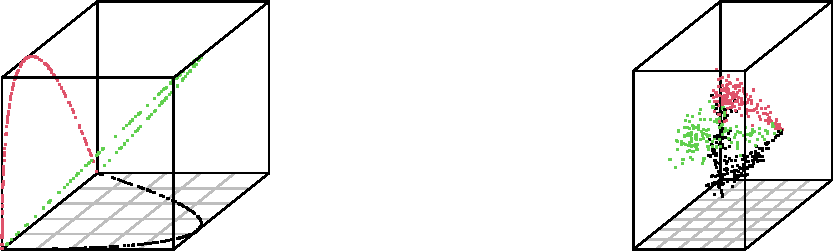
\includegraphics{draft_files/figure-latex/three-curves-1} 

}

\caption{Latent vectors (left) and ASE (right) of one realization of the mixture model in the simulation setup with $K=3$ manifolds.}\label{fig:three-curves}
\end{figure}

As in the previous setup, we set \(n = 128, 256, 512, 1024, 2048\), and we started with completely random initializations as well as initializations in which we know \(4\) or \(8\) labels from each community.
For each setting, we simulated 50 replicates.
Since the curves meet at the origin, we forced the fitted Bezier curves to meet at the origin as well by fixing \(p_k^{(0)} = (0, 0, 0)\) for each \(k\).
Figure \ref{fig:sim-curves-3} shows the median and interquartile ranges for the error rates for each \(n\) and \emph{a priori} known labels per community.
As in the previous \(K = 2\) simulations, the results suggest that for sufficient \(n\), we do not benefit from having more known labels, but having a few results in greatly improved performance. Unlike in the previous setup, random initialization results in low community detection error rates, close to the semi-supervised setups for larger \(n\).

\begin{figure}[H]

{\centering 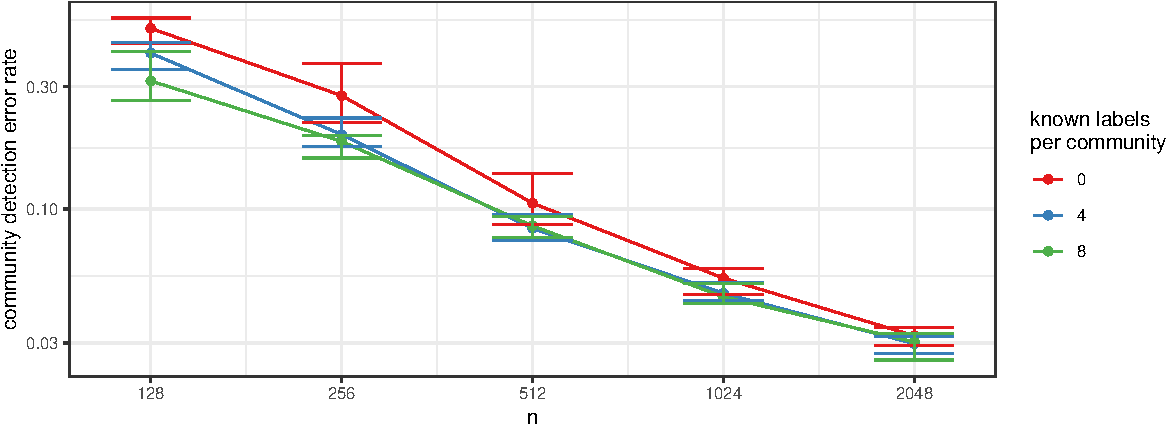
\includegraphics{draft_files/figure-latex/sim-curves-3-1} 

}

\caption{Median and IQR error rates over 50 replicates in the simulation setup for $K = 3$ curves.}\label{fig:sim-curves-3}
\end{figure}

\hypertarget{applications-1}{%
\subsection{Applications}\label{applications-1}}

In the first example, we applied \(K\)-curves clustering (algorithm \ref{alg:kcurves}) to the Macaque visuotactile brain areas and connections network \citep{https://doi.org/10.1111/j.1460-9568.2006.04678.x}, which is visualized in figure \ref{fig:macaque-graph}.
In this graph, there are 45 vertices which each correspond to a brain area, and the communities represent each area's tactile function.
Applying an ASE with \(p = 2\) and \(q = 0\) to this graph results in an embedding that appears to fall approximately on two curves (figure \ref{fig:macaque-ase}) which intersect at the origin.
Figure \ref{fig:macaque-fitted} shows the result of \(K\)-curves clustering on this graph,
which yields a 4.4\% error rate.

\begin{figure}[H]

{\centering 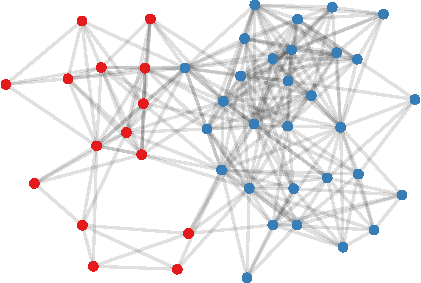
\includegraphics{draft_files/figure-latex/macaque-graph-1} 

}

\caption{Macaque visuotactile brain areas and connections network. The vertices represent brain areas.}\label{fig:macaque-graph}
\end{figure}

\begin{figure}[H]

{\centering 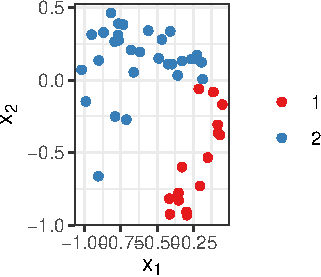
\includegraphics{draft_files/figure-latex/macaque-ase-1} 

}

\caption{ASE on the Macaque brain areas network. The embedding suggests a community-wise manifold structure.}\label{fig:macaque-ase}
\end{figure}

\begin{figure}[H]

{\centering 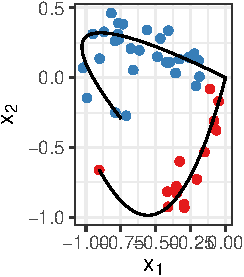
\includegraphics{draft_files/figure-latex/macaque-fitted-1} 

}

\caption{$K$-means clustering on the ASE of the Macaque brain areas network. The embedding vectors are colored by predicted label.}\label{fig:macaque-fitted}
\end{figure}

In the second example, we considered the Harry Potter enmity graph \citep{harrypotter}, visualized in figure \ref{fig:hp}.
This graph does not come with ground truth labels.
\citet{rubindelanchy2017statistical} and \citet{SannaPassino2022} analyzed this graph as a GRDPG, and the ASE suggests that an appropriate model for this graph is a disassortative DCBM with \(K = 2\) communities.
Indeed, if we construct an ASE with \(p = 1\) and \(q = 1\) and label the points by character name, we see embedding vectors lie neatly along two rays emitting from the origin, with one ray populated by protagonists and another ray populated by antagonists (figure \ref{fig:hp-ase}).
Nevertheless, we tried fitting an MBM on this graph via \(K\)-curves clustering.
Since the DCBM is a special case of the MBM, it should result in at least as good of a fit as the DCBM.
We initialized \(K\)-curves clustering by specifying that Lord Voldemort is in one community and Harry Potter is in another, with the other vertices not known \emph{a priori}.
The fitted quadratic curves are illustrated in figure \ref{fig:hp-kcurves}, which indeed appear to be very close to linear.

\begin{figure}[H]

{\centering 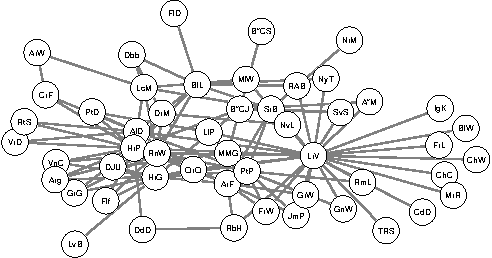
\includegraphics{draft_files/figure-latex/hp-1} 

}

\caption{Harry Potter enmity graph. The vertices represent characters and the edges represent whether pairs of characters are enemies.}\label{fig:hp}
\end{figure}

\begin{figure}[H]

{\centering 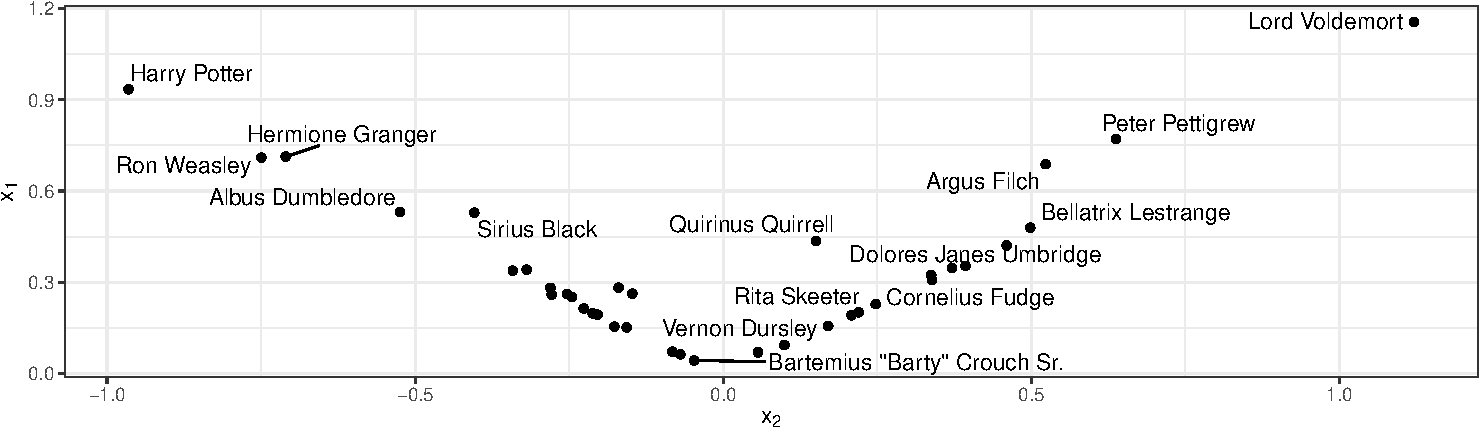
\includegraphics{draft_files/figure-latex/hp-ase-1} 

}

\caption{ASE of the Harry Potter emnity graph. The way in which the embedding vectors are organized suggest that a DCBM is an appropriate model for this graph.}\label{fig:hp-ase}
\end{figure}

\begin{figure}[H]

{\centering 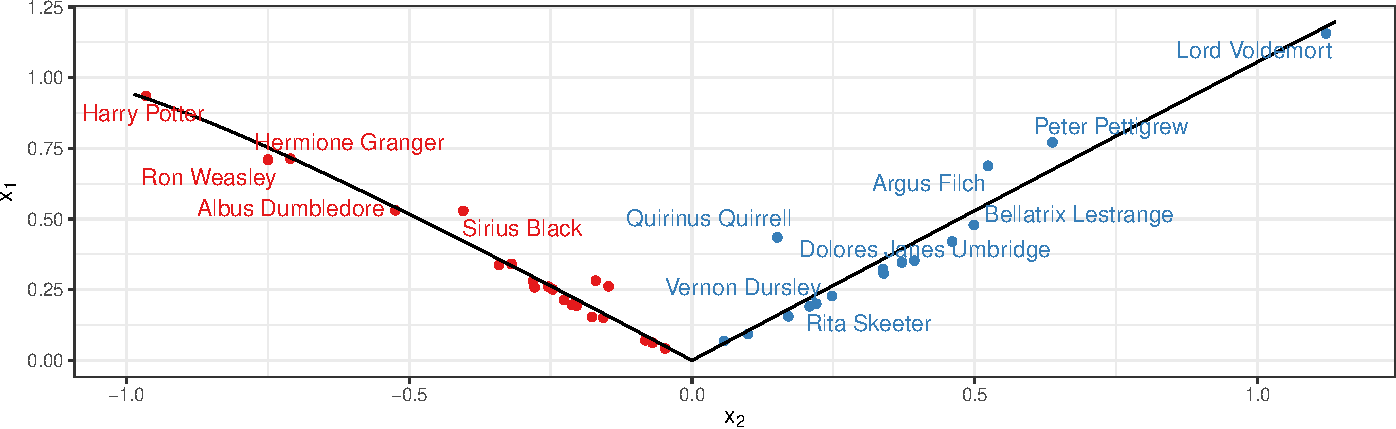
\includegraphics{draft_files/figure-latex/hp-kcurves-1} 

}

\caption{ASE of the Harry Potter emnity graph with quadratic Bezier curves fitted via $K$-curves clustering. The embedding vectors are colored by predicted label.}\label{fig:hp-kcurves}
\end{figure}

In the final example, we examined the \emph{Drosophila} connectome graphs \citep{Eichler141762}, which has been studied as a GRDPG by \citet{athreya2017statistical}, \citet{https://doi.org/10.48550/arxiv.1705.03297}, and \citet{SannaPassino2022}.
This dataset consists of two graphs representing two networks of neurons, one for each hemisphere of the \emph{Drosophila} brain.
In these graphs, each vertex is a neuron, and the labels correspond to one of four neuron types (Kenyon Cells, Input Neurons, Output Neurons, and Projection Neurons).
The resulting graphs are illustrated in figure \ref{fig:mbconnectome-graph}.

The ASE in two dimensions suggest that the MBM with one dimensional quadratic manifolds is an appropriate model for these graphs (figure \ref{fig:mbconnectome-ase}).
Fitting two quadratic Bezier curves to the ASEs (figure \ref{fig:mbconnectome-kcurves}) results in 72.2\% accuracy for the left hemisphere connectome and 83.6\% accuracy for the right hemisphere connectome.
The curves were fitted on three-dimensional ASEs with \(p = 2\) and \(q = 1\), which were chosen based on setting the threshold \(|\lambda_i| > \sqrt{n}\) where \(\lambda_i\) is the \(i\)\textsuperscript{th} greatest eigenvalue.
Figure \ref{fig:mbconnectome-kcurves} shows the embedding and curves projected to the first two components.

\begin{figure}[H]

{\centering \includegraphics{draft_files/figure-latex/mbconnectome-graph-1} 

}

\caption{Graphs of the Drosophila connectomes. The left and right are of the left and right hemispheres, respectively. Each vertex represents a neuron, which are labeled by neuron type.}\label{fig:mbconnectome-graph}
\end{figure}

\begin{figure}[H]

{\centering 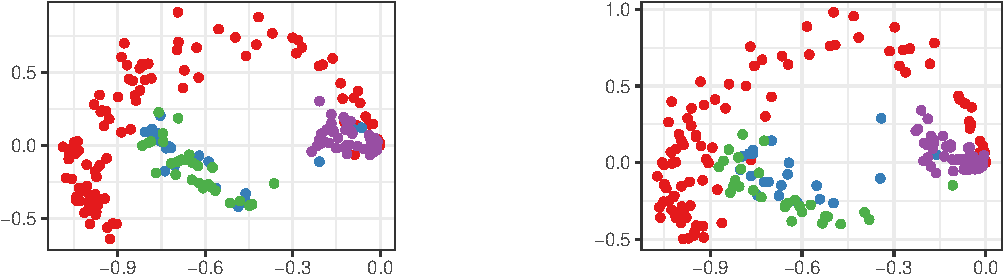
\includegraphics{draft_files/figure-latex/mbconnectome-ase-1} 

}

\caption{ASEs of the Drosophila connectome graphs. The embedding vectors are labeled by neuron type.}\label{fig:mbconnectome-ase}
\end{figure}

\begin{figure}[H]

{\centering 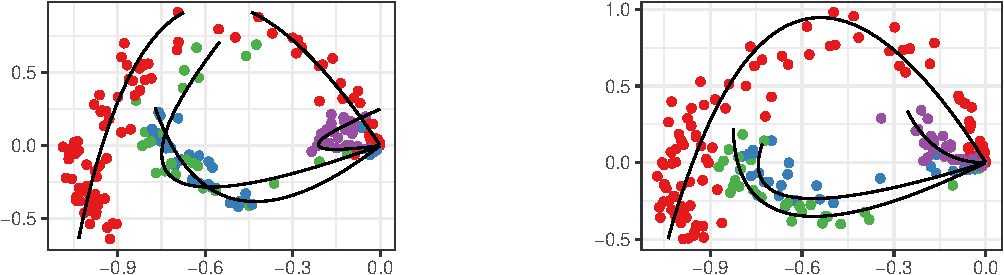
\includegraphics{draft_files/figure-latex/mbconnectome-kcurves-1} 

}

\caption{ASEs of the Drosophila connectome graphs with quadratic Bezier curves fitted via $K$-curves clustering. The embedding vectors are colored by predicted label.}\label{fig:mbconnectome-kcurves}
\end{figure}

\hypertarget{conclusions}{%
\subsection{Conclusions}\label{conclusions}}

\newpage

\section*{Appendix A: Proofs of Theorems from Section 3}

Let \(V_n\) and \(\hat{V}_n\)
be the \(n \times K^2\) matrices whose columns are the eigenvectors of \(P\) and \(A\) corresponding to the
\(K^2\) largest eigenvalues (in modulus), respectively.
We first state an important technical lemma for bounding the maximum
\(\ell_2\) norm difference between the rows of \(\hat{V}_n\) and
\(V_n\). See \citet{cape_biometrika} and
\citet[Lemma~5]{rubindelanchy2017statistical} for a proof.

\begin{lemma}
\label{lem:technical}
Let $A \sim \mathrm{PABM}(\{\lambda^{(k \ell \ell)}\}_{K})$ be a $K$-blocks
PABM graph on $n$ vertices and let \(V\) and \(\hat{V}\)
be the $n \times K^2$ matrices whose columns are the eigenvectors of 
\(P\) and \(A\) corresponding to the
$K^2$ largest eigenvalues in modulus, respectively.
Let \(v_i^\top\) and \(\hat{v}_i^\top\) denote the $i$th 
row of \(V\) and \(\hat{V}\), respectively. 
Then there exists a constant $c > 1$ and an orthogonal matrix $W$ such
that with high probability,
$$\max_{i} \|W \hat{v}_i - v_i\|  = O\Big(\frac{\log^{c}n}{n \sqrt{\rho_n}} \Big).$$
In particular we can take $c = 1 + \epsilon$ for any $\epsilon > 0$. 
\end{lemma}

\begin{proof}[Proof of theorem~\ref{thm:osc}]
Recall the notations in lemma~\ref{lem:technical} and note that,
under our assumption that the latent vectors $\lambda^{(k \ell)}$
are all homogeneous, we have $\max_{i} \|v_i\| =
O(n^{-1/2})$. 

Next recall theorem~\ref{thm:osc-p}; in particular $B_{ij} = nv_i^{\top}
v_j$. 
We therefore have
\[\begin{split}
\max_{ij} |\hat{B}_{ij} - B_{ij}| &= \max_{ij} n |\hat{v}_i^\top \hat{v}_j -
v_i^\top v_j| \\
& \leq n \max_{ij} |\hat{v}_i^\top W W^\top \hat{v}_j -
v_i^\top v_j| \\
& \leq n \max_{i,j} \Bigl(\|W^{\top} \hat{v}_i - v_i\| \times \|\hat{v}_j\|
+ \|W^{\top} \hat{v}_j - v_j\| \times \|v_i\|\Bigr) \\
& \leq n \Bigl(\max_{ij}  \|W \hat{v}_i  - v_i \|^2 +  \|W
\hat{v}_i  - v_i \| \times \|v_j\| +  \|W \hat{v}_j  - v_j \| \times \|v_i\|\Bigr) 
\\ &
\leq n \max_{i} \|W \hat{v}_i  - v_i \|^2 + 2n \max_{i}
\|W \hat{v}_i  - v_i \| \times \max_{j} \|v_j\|
\\
& = O \Big( \frac{\log^{c}{n}}{n^{1/2} \rho_n^{1/2}} \Big)
\end{split}\]
with high probability.
Theorem~\ref{thm:osc} follows from the above bound together with the
conclusion in theorem~\ref{thm:osc-p} that $B_{ij} = 0$ whenever vertices $i$ and $j$
belongs to different communities. 
\end{proof}

We now provide a proof of theorem \ref{thm:ssc}. Our proof is based on verifying the sufficient conditions given in theorem 6 of \citet{jmlr-v28-wang13} under which sparse subspace clustering based on solving the optimization problem in equation \eqref{eq:ssc} yields an affinity matrix \(B = |C| + |C^{\top}|\) satisfying the subspace detection property of definition \ref{def:subspace_detection}.
We first recall a few definitions used in \citet{soltanolkotabi2012} and \citet{jmlr-v28-wang13};
for ease of exposition, these definitions are stated using the notations of the current paper and we will drop the explicit dependency on \(n\) from our eigenvectors \(\hat{V}\) of \(A\) and \(V\) of \(P\).

\begin{definition}[Inradius]
\label{def:inradius}
The inradius of a convex body $\mathcal{P}$, denoted by $r(\mathcal{P})$, is
defined as the radius of the largest Euclidean ball inscribed in $\mathcal{P}$.
Let $X$ be a $n \times d$ matrix with rows $x_1, x_2, \dots,
x_n$. We then define, with a slight abuse of notation, $r(X)$ as the
inradius of the convex hull formed by $\{\pm x_1, \pm x_2, \dots, \pm x_n\}$. 
\end{definition}

\begin{definition}[Subspace incoherence]
\label{def:subspace_incoherence}
Let $\hat{V}$ be the eigenvectors of $A$
corresponding to the $K^2$ largest eigenvalues in modulus. Let
$\hat{V}^{(k)}$ denote the matrix formed by keeping only the rows of
$\hat{V}$ corresponding to the $k^{th}$
community and let $\hat{V}^{(-k)}$ denote the matrix formed by
omitting the rows of $\hat{V}$
corresponding to the $k^{th}$ community. Let $(\hat{v}_i^{(k)})^\top$ denote
the $i$th row of $\hat{V}^{(k)}$ and $\hat{V}_{-i}^{(k)}$ be $\hat{V}^{(k)}$ with
the $i^{th}$ row omitted. Let $V$, $V^{(k)}$, $V^{(-k)}$, and
$v_i^{(k)}$ be defined similarly using the eigenvectors $V$ of
$P$. Finally let $\mathcal{S}^{(k)}$ be the vector space spanned by the
rows of $V^{(k)}$. 

Now define $\nu_{i}^{(k)}$ for $k = 1,2,\dots,K$ and $i =
1,2,\dots,n_{k}$ as the solution of the following optimization problem
$$\nu_{i}^{(k)} = \max_\eta (\hat{v}_i^{(k)})^\top \eta - \frac{1}{2
\lambda} \eta^\top \eta, \quad \text{subject to $\|V_{-i}^{(k)}
\eta\|_\infty \leq 1$.}$$
Given $\nu_i^{(k)}$, let $\mathbb{P}_{\mathcal{S}^{(k)}}(\nu_i^{(k)})$
be the vector in $\mathbb{R}^{K^2}$ corresponding to the orthogonal projection of $\nu_i^{(k)}$ onto the vector space
$\mathcal{S}^{(k)}$ and define the projected dual direction $w_{i}^{(k)}$
as
$$w_i^{(k)} =
\frac{\mathbb{P}_{\mathcal{S}^{(k)}}(\nu_i^{(k)})}{\|\mathbb{P}_{\mathcal{S}^{(k)}}(\nu_i^{(k)})\|}.$$
Now let $W^{(k)} = \bigl[ w_1^{(k)} \mid \cdots \mid w_{n_k}^{(k)} \bigr]^\top$
and define the subspace incoherence for $\hat{V}^{(k)}$ by
$$\mu^{(k)} = \mu(\hat{V}^{(k)}) = \max\limits_{v \in V^{(-k)}} \|W^{(k)} v\|_\infty.$$
\end{definition}

\begin{proof}[Proof of theorem \ref{thm:ssc}]
For a given $k = 1,2\dots,K$, let $r^{(k)} = \min_{i}r(V_{-i}^{(k)})$ be inradius of the convex hull formed by
the rows of $V_{-i}^{(k)}$ and let $r_* = \min_{k} r^{(k)}$. Then Theorem~6 in
\citet{jmlr-v28-wang13} states that there exists a $\lambda > 0$
such that $\sqrt{n} \hat{V}$ satisfies the subspace detection property in definition \ref{def:subspace_detection} whenever the following two conditions are satisfied: 
\begin{gather}
\label{eq:cond1}
\mu^{(k)} < r^{(k)} \quad \text{for all $k = 1,2,\dots,K$}, \\
\label{eq:cond2}
\max_{i} \|W \hat{v}_{i} - v_{i}\| \leq \min_{k} \frac{r_*(r^{(k)} -
\mu^{(k)})}{2 + 7 r^{(k)}}.
\end{gather}
We now verify that for sufficiently large n, equation \eqref{eq:cond1} and equation~\eqref{eq:cond2}
holds with high probability.

{\bf Verifying equation \eqref{eq:cond1}}. If $n$ is sufficiently large then
there are enough vertices in each community $k$ so that
$\mathrm{span}(V_{-i}^{(k)}) = \mathcal{S}^{(k)}$ for all $i$ and hence
\(r^{(k)} = \min_{i} r(V_{-i}^{(k)}) > 0\) for
all $k = 1,2,\dots,K$. 

Next, by theorem \ref{thm:osc-p} we have that the subspaces
$\{\mathcal{S}^{(1)}, \dots, \mathcal{S}^{(K)}\}$
are mutually orthogonal, i.e., $v^{\top} w = 0$ for all $v \in
\mathcal{S}^{(k)}$ and $w \in \mathcal{S}^{(\ell)}$ with $k \not =
\ell$. Now let $z \in \mathbb{R}^{K^2}$ be arbitrary and let
$\tilde{z} = \mathbb{P}_{\mathcal{S}^{(k)}} z$ be the projection of
$z$ onto $\mathcal{S}^{(k)}$. We then have $v^{\top} \tilde{z} =
0$ for all $v \in V^{(-k)}$. Because $z$ is arbitrary, this implies 
$\|W^{(k)} v\|_{\infty} = 0$ for all $v
\in V^{(-k)}$ and hence $\mu^{(k)} = 0$ for all $k
=1,2,\dots,K$. Therefore $\mu^{(k)} < r^{(k)}$ for all $k =
1=2,\dots,K$ as desired.

{\bf Verifying equation \eqref{eq:cond2}}.
Let $\delta = \max_{i} \sqrt{n} \|W \hat{v}_{i} - v_{i}\|$. 
Then from lemma \ref{lem:technical}, we have \(\delta \stackrel{a.s.}{\to} 0\) and hence
$$\delta < \min_{k} \frac{r_* (r^{(k)} - \mu^{(k)})}{2 + 7 r^{(k)}}$$
asymptotically almost surely. 

In summary $\sqrt{n} \hat{V}$ satisfies the subspace detection property with probability converging to $1$ as \(n \to \infty\).
\end{proof}

\begin{remark}
Theorem 6 of \citet{jmlr-v28-wang13} assumes that each row $v_i$
of $V$ has unit norm, i.e., $\|v_{i}\| = 1$  for all $i$. 
This assumption has the effect of scaling the $r^{(k)}$ so that $r^{(k)} \leq 1$ for all $k = 1,2,\dots,K$. 
We emphasize that this assumption has no effect on the proof of Theorem \ref{thm:ssc}. 
Indeed, because $\mu^{(k)} = 0$ for all $k$, as long as the rows of $V^{(k)}$ spans the subspace $\mathcal{S}^{(k)}$, then $a r^{(k)} > \mu^{(k)}$ for any scalar $a > 0$. 
\end{remark}

\begin{proof}[Proof of Theorem \ref{thm:param-est}] 
Let \(P\) be organized by community such that \(P^{(k \ell)}\) denote the $n_k \times n_{\ell}$ matrix obtained by keeping only the rows of $P$ corresponding to vertices in community $k$ and the columns of $P$ corresponding to vertices in community $\ell$. 
We define $A^{(k \ell)}$ analogously. 
Recall that $P^{(k \ell)} = \lambda^{(k \ell)} (\lambda^{(\ell k)})^{\top}$ for all $k, \ell$. 
We now consider estimation of $P^{(k \ell)}$ for the cases when $k = \ell$ versus when $k \not = \ell$.

\emph{Case \(k = l\)}. 
Let $P^{(kk)} = \sigma_{kk}^2 u^{(kk)} (u^{(kk)})^\top$ be the singular value decomposition of $P^{(kk)}$. 
We can then define $\tilde{\lambda}^{(kk)} = \sigma_{kk} u^{(kk)}$. 
Now let $\hat{U}^{(kk)} \hat{\Sigma}^{(kk)} (\hat{U}^{(kk)})^\top$ be the singular value decomposition of \(A^{(kk)}\), and let $\hat{\sigma}_{kk}^2 \hat{u}^{(kk)} (\hat{u}^{(kk)})^\top$ be the best rank-one approximation of $A^{(kk)}$. 
Define \(\hat{\lambda}^{(kk)} = \hat{\sigma}_{kk} \hat{u}^{(kk)}\). 
Then \(\hat{\lambda}^{(kk)}\) is the adjacency spectral embedding approximation of \(\lambda^{(kk)}\), and by Theorem 5 of \citet{rubindelanchy2017statistical}, we have
$$\|\hat{\lambda}^{(kk)} - \lambda^{(kk)}\|_{\infty} = O\Bigl(\frac{\log n_k}{\sqrt{n_k}}\Bigr)$$
with high probability. 
Here $\|\cdot\|_{\infty}$ denote the $\ell_{\infty}$ norm of a vector.

\emph{Case \(k \neq l\)}. 
Let \(P^{(k \ell)} = \sigma_{k \ell}^2 u^{(k \ell)} (v^{(k \ell)})^\top\) and \(P^{(\ell k)} = \sigma_{kl}^2 u^{(\ell k)} (v^{(\ell k)})^\top\) be the singular value decompositions and note that \(\sigma_{k \ell} = \sigma_{\ell k}\), \(u^{(k \ell)} = v^{(\ell k)}\), and \(v^{(k \ell)} = u^{(\ell k)}\). 
Now define \(\lambda^{(k \ell)} = \sigma_{k \ell} u^{(k \ell)}\) and \(\lambda^{(\ell k)} = \sigma_{k \ell} v^{(k \ell)}\).

Next consider the Hermitian dilation
\[
M^{(k \ell)} = 2 \begin{bmatrix} 0 & P^{(k \ell)} \\ P^{(\ell k)} & 0 \end{bmatrix}
\]
which is a symmetric \((n_k + n_\ell) \times (n_k + n_\ell)\) matrix. 
The eigendecomposition of \(M^{(k \ell)}\) is then

\[M^{(k \ell)} = 
\begin{bmatrix} u^{(k \ell)} & -u^{(k \ell)} \\ v^{(k \ell)} & v^{(k \ell)} \end{bmatrix} \times 
\begin{bmatrix} \sigma^2_{kl} & 0 \\ 0 & -\sigma^2_{kl} \end{bmatrix} \times
\begin{bmatrix} u^{(k \ell)} & -u^{(k \ell)} \\ v^{(k \ell)} & v^{(k \ell)} \end{bmatrix}^\top\]
Thus treating \(M^{(k \ell)}\) as the edge probability matrix of a GRDPG, we have latent positions in \(\mathbb{R}^2\) given by the $(n_k + n_{\ell}) \times 2$ matrix
\[\Lambda^{(k \ell)} = \begin{bmatrix} 
\sigma_{k \ell} u^{(k \ell)} & \sigma_{k \ell} u^{(k \ell)} \\ 
\sigma_{k \ell} v^{(k \ell)} & -\sigma_{k \ell} v^{(k \ell)} 
\end{bmatrix} = 
\begin{bmatrix} 
\lambda^{(k \ell)} & \lambda^{(k \ell)} \\ 
\lambda^{( \ell k)} & -\lambda^{( \ell k)} 
\end{bmatrix}.\]
Now consider
\[\hat{M}^{(k \ell)} = \begin{bmatrix} 0 & A^{(k \ell)} \\ A^{(\ell k)} & 0 \end{bmatrix}\]

We can then view \(\hat{M}^{(k \ell)}\) as an adjacency matrix drawn from
the edge probabilities matrix \(M^{(k \ell)}\). Now suppose that the adjacency spectral
embedding of $\hat{M}^{(k \ell)}$ is represented as the $(n_k +
n_{\ell}) \times 2$ matrix
\[\hat{\Lambda}^{(k \ell)} = \begin{bmatrix} 
\hat{\lambda}^{(k \ell)} & \hat{\lambda}^{(k \ell)} \\ 
\hat{\lambda}^{(\ell k)} & -\hat{\lambda}^{(\ell k)} 
\end{bmatrix}\]
where each \(\hat{\lambda}^{(k \ell)}\) is defined as in Algorithm 3. Then
by Theorem 5 of \citet{rubindelanchy2017statistical}, there
exists an indefinite orthogonal transformation $W^{*}$ such that,  with
high probability,
$$\max_{i} |W^{*} \hat{\Lambda}_{i}^{(k \ell)} - \Lambda_{i}^{(k \ell)} \| =
O\Bigl(\frac{\log (n_k + n_{\ell})}{\sqrt{n_k + n_{\ell}}}\Bigr)$$
with high probability. Here $\Lambda_{i}^{(k \ell)}$ and
$\hat{\Lambda}_i^{(k \ell)}$ denote the $i$th rows of $\Lambda^{(k
\ell)}$ and $\hat{\Lambda}^{(k \ell)}$, respectively. 

Furthermore, by looking at the proof of Theorem~5 in
\citep{rubindelanchy2017statistical}, we see that $W^{*}$ is also
blocks diagonal with $2$ blocks where the positive eigenvalues of $M^{(k \ell)}$
forming a block and the negative eigenvalues of $M^{(k \ell)}$ forming
the remaining block. 
Because $M^{(k \ell)}$ has one positive eigenvalue and one negative
eigenvalue, we see that $W^{*}$ is necessarily of the form $W^{*}
= \Bigl[\begin{smallmatrix} 1 & 0 \\ 0 & - 1\end{smallmatrix}\Bigr]$
Using this form for $W^{*}$, we obtain
$$\max\{\|\hat{\lambda}^{(k \ell)} - \lambda^{(k \ell)}\|_{\infty},
\|\hat{\lambda}^{(\ell k)} - \lambda^{(\ell k)}\|_{\infty}\}  =
O\Bigl(\frac{\log(n_k + n_{\ell})}{\sqrt{n_k + n_{\ell}}}\Bigr)$$
with high probability. Combining this bound with the bound for
$\|\hat{\lambda}^{(kk)} - \lambda^{(kk)}\|_{\infty}$ given above
yields equation~\eqref{eq:param-est} in theorem~\ref{thm:param-est}. 
\end{proof}

\section*{Appendix B: Proofs of Theorems from Section 4}

\begin{lemma}
\label{lemma:no-noise}
Let $x_1, ..., x_n$ be drawn from $K$ compact, connected manifolds $\mathcal{M}_1$, ..., $\mathcal{M}_K$ each with probability measures $F_1$, ..., $F_K$, and the manifolds are separated by distance at least $\delta > 0$. 
Suppose that for any $\epsilon > 0$ and $x$ drawn from each $F_k$, on $\mathcal{M}_k$, $F(B(x, \epsilon)) > 0$ where $B(x, \epsilon)$ is the open ball of radius $\epsilon$ centered at $x$. 
Let $E_n(\eta)$ denote the event that an $\eta$-neighborhood graph constructed from $x_1, ..., x_n$ is comprised of exactly $K$ disjoint subgraphs that map to each of the $K$ manifolds. 
Then if each $n_k \to \infty$ as $n \to \infty$, $\lim\limits_{n \to \infty} P(E_n(\eta)) = 1$ for each $\eta \in (0, \delta)$. 
\end{lemma}

\begin{proof}
It is clear that if $\eta \in (0, \delta)$, an $\eta$-neighborhood graph constructed from the sample will always consist of at least $K$ disjoint subgraphs for which no subgraph contains vertices belonging to points from two different manifolds. 
Then it is sufficient to show that for a sufficiently large $n$, any $\eta$-neighborhood graph (where $\eta \in (0, \delta)$) will achieve $E_n$. 

Define each $E_{n_k}^{(k)}(\eta)$ as the event that if a sub-sample of size $n_k$ drawn from manifold $\mathcal{M}_k$, every $x \in \mathcal{M}_k$ is within distance $\eta$ of some $x_j$ of the sub-sample. 
Then if $E_{n_k}^{(k)}(\eta)$ is true, the $\eta$-neighborhood graph results in a connected subgraph for points within the $k^{th}$ manifold. 
By lemma 2 of \citet{trosset2020rehabilitating}, $P((E_{n_k}^{(k)}(\eta))^c) \leq \ell_k (1 - b_k)^{n_k}$ for some $\ell_k \in \mathbb{N}$ and $b_k \in (0, 1]$. 
If each $E_{n_k}^{(k)}(\eta)$ is true, then $E_n$ is achieved, so $E_n(\eta) = \bigcap_k E_{n_k}^{(k)}(\eta))$. 
$\bigcap_k E_{n_k}^{(k)}(\eta) = \Big( \bigcup_k (E_{n_k}^{(k)}(\eta))^c \Big)^c$, so it is sufficient to show $\lim\limits_{n \to \infty} P \big( \bigcup_k (E_{n_k}^{(k)}(\eta))^c \big) \to 0$. 

$$
\begin{aligned}
P \big( \bigcup_k(E_{n_k}^{(k)})^c \big) & \leq \sum_k P \big((E_{n_k}^{(k)})^c \big) \\
& \leq \sum_k \ell_k (1 - b_k)^{n_k} \\
& \leq K \ell_{\max} (1 - b_{\min})^{n_{\min}},
\end{aligned}
$$

which tends to $0$ as $n \to \infty$. 
\end{proof}

\begin{proof}[Proof of theorem \ref{theorem:nonintersect-grdpg}]
Define $E_n(\eta)$ as in lemma \ref{lemma:no-noise} for manifolds $Q_n(\mathcal{M}_1), ..., Q_n(\mathcal{M}_K)$ and each $e_i = \hat{x}_i - Q_n x_i$ where $\hat{x}_i$ is the $i^{th}$ embedding vector and $Q_n$ is some indefinite orthogonal transformation as in \citet{rubindelanchy2017statistical}. 
Since $Q_n$ is a linear map, for any $\eta \in (0, \|Q_n\| \delta)$, $P(E_n(\eta)) \to 1$ as $n \to \infty$. 
Let $\epsilon_i = \|e_i\|$, $\epsilon = \max_i \epsilon_i$, and $C_n = \|Q_n\|$. 

$A_n(\eta)$ is true if $\eta < \min\limits_{k, \ell} \min\limits_{x_i \in \mathcal{M}_k, x_j \in \mathcal{M}_\ell} \|\hat{x}_i - \hat{x}_j\|$, which is defined as event $D_n(\eta)$, and $\eta \geq \max\limits_k \max\limits_{x_i, x_j \in \mathcal{M}_k} \|\hat{x}_i - \hat{x}_j\|$, which is defined as event $\hat{E}_n(\eta)$.

For any $x_i, x_j$ from different manifolds, $\|\hat{x}_i - \hat{x}_j\| \geq C_n \delta - 2 \epsilon$ if $2 \epsilon \leq C_n \delta$. 
By theorem 3 of \citet{rubindelanchy2017statistical}, for some finite $M > 0$, $P \big(\epsilon < M \frac{\log^c n}{\sqrt{n}} \big) \to 1$ as $n \to \infty$, so $P(C_n \delta < 2 \epsilon) \leq P(C_n \delta < 2 M n^{1/2} \log^c n) \to 0$ since $C_n \delta > 0$. 
Then since $P(C_n \delta - 2 \epsilon > 0) \to 1$, there is an $\epsilon \in (0, C_n \delta - 2 \epsilon)$ with probability 1. 
Thus, $P(D_n(\eta)) \to 1$. 

Then to show that $P(A_n) \to 1$: 

$$
\begin{aligned}
P(A_n) & = P(\hat{E}_n(\eta) \cap D_n) \\
& = P((\hat{E}_n^c(\eta) \cup D_n^c)^c) \\
& = 1 - P(\hat{E}_n^c(\eta) \cup D_n^c) \\
& \geq 1 - P(\hat{E}_n^c(\eta)) - P(D_n^c) \\ 
& = P(\hat{E}_n(\eta)) + P(D_n) - 1,
\end{aligned}
$$
which tends toward $1$ as $n \to \infty$ since both $P(E_n(\eta))$ and $P(D_n)$ tend toward $1$ as $n \to \infty$. 
\end{proof}

\begin{proof}[Proof of theorem \ref{thm:kcurves-semisupervised}]
Let $\hat{X}$ with rows $\hat{x}_i^\top$ be the ASE of $A$ drawn from an MBM in which each $g_k(t) = g(t; p_k)$ is a Bezier curve of order $R$. 
Define the ASE error as $\epsilon_i = \|Q \hat{x}_i - x_i\|$ and $\epsilon = \max_i \epsilon_i$ where $Q$ is the appropriate indefinite orthogonal transformation for the ASE. 
By \citet{rubindelanchy2017statistical}, $\epsilon = O_P \bigg(\frac{\log^c n}{\sqrt{n}} \bigg)$. 

The statement of the theorem assumes that for each community $k$, there at least $R + 1$ points with known label $k$. 
For simplicity, suppose we have exactly $R + 1$ (if there are more, then discard the rest). 
Then for each community $k$, it is possible to fit a polynomial of order $R$ that goes through each of the $R + 1$ known points exactly, yielding $g(t; \hat{p}_k)$, where $\hat{p}_k$ are the fitted coefficients of the Bezier polynomial. 
Use the fitted Bezier curves to define $\delta_k(t) = \|Q g(t; \hat{p}_k) - g(t; p_k)\|$, $\delta_k = \max_t \delta_k(t)$, and $\delta = \max_k \delta_k$. 
Since $P(\epsilon < M n^{-1/2} \log^c n) \to 1$ for constants $M, c > 0$, 
$P(\delta_k < M n^{-1/2} \log^c n) \to 1$ for each $k$. 
Since $\epsilon_i$ describes the error between each embedding point and its corresponding latent vertex, and $\delta_k(t_i)$ describes the error between the fitted curve and its corresponding true curve in the latent space, 
$$L < \frac{1}{n} \sum_i \epsilon_i + \delta_{z_i}(t_i) < \frac{1}{n} n (\epsilon + \delta) = \epsilon + \delta.$$ 
Then as $n \to \infty$, 
$$P(L < 2 M n^{-1/2} \log^c n) > P(\epsilon + \delta < 2 M n^{-1/2} \log^c n) \to 1.$$
\end{proof}

\newpage

\section*{Appendix C: Details on Fitting Bezier Curves to Noisy Data}

The curve fitting step in algorithm \ref{alg:kcurves} requires estimation of some \(g: [0, 1] \to \mathbb{R}^d\) for each subset of points corresponding to each label.
One choice of curve is the Bezier polynomial.
The Bezier polynomial of order \(R\) is defined by function \(g\) with parameters \(p\) such that
\[g(t; p) = \sum_{r=0}^R p^{(r)} \binom{R}{r} t^r (1-t)^{R-r}\]
where the Bezier coefficients \(p^{(r)}\) are vectors in \(\mathbb{R}^d\), and \(p = \Big[ p^{(0)} \mid \cdots \mid p^{(R)} \Big]^\top\).

The general idea behind Bezier curve fitting to noisy data is as follows:
We wish to minimize the squared loss function
\begin{equation}
\label{eq:bezier-ls}
L(p, t; X) = \sum_i \|x_i - g(t_i; p)\|^2.
\end{equation}
Suppose that we know the timepoints \(t_1, ..., t_n\) which we wish to use to fit Bezier coefficients \(p^{(0)}, ..., p^{(R)}\) to vectors \(x_1, ..., x_n \in \mathbb{R}^d\) lying on or near a Bezier curve of order \(R\).
The squared loss then can be written as
\[L(p; t, X) = \|X - T p\|^2,\]
where \(p\) is defined as before, \(T\) is an \(n \times (R+1)\) matrix such that \(T_{ir} = \binom{R}{r} t_i^r (1-t_i)^{R-r}\), and \(X = \Big[ x_1 \mid \cdots \mid x_n \Big]\).
Then the least squares estimates for the Bezier coefficients \(p\) is simply the linear least squares estimate
\begin{equation}
\label{eq:bezier-p-fit}
\hat{p} = (T^\top T)^{-1} T^\top X.
\end{equation}

On the other hand, suppose that we know the Bezier coefficients \(p = \Big[ p^{(0)} \mid \cdots \mid p^{(R)} \Big]^\top\), and we wish to fit timepoints \(t_1, ..., t_n\) to vectors \(x_1, ..., x_n\) lying on or near a Bezier polynomial of order \(R\).
In this setting, we can fit each individual \(t_i\) independently by minimizing \(L(t_i; p, x_i) = \|x_i - g(t_i; p)\|^2\) for each \(t_i\).
If \(g(t_i; p, x_i)\) is a polynomial of order \(R\), then \(\dot{L}(t_i; p, x_i)\) is also a polynomial, of order \(2 R - 1\).
Minimizing \(L(t_i; p, x_i)\) then simply involves finding the roots of \(\dot{L}(t_i; p, x_i)\) and choosing the root with the smallest objective value (in practice, the endpoints \(t_i = 0\) and \(t_i = 1\) are also checked).
For the Bezier curve of order \(R\), the full polynomial is given by:
\begin{equation}
\label{eq:dbezier}
\dot{L}(t_i; p, x_i) = \bigg(\sum_{r=0}^R \binom{R}{r} (-1)^r c_r t^r \bigg) \bigg(\sum_{r=0}^{R-1} \binom{R-1}{r} (-1)^r c_{r+1} t^r \bigg),
\end{equation}
where \(c_R = \sum_{r=0}^R (-1)^{R-r} \binom{R}{r} p^{(r)}\).
The full Bezier polynomial fitting method is detailed in algorithm \ref{alg:bezier-fit}.

\begin{algorithm}[h]
\label{alg:bezier-fit}
\DontPrintSemicolon
\SetAlgoLined
\setstretch{1.5}
\KwData{$x_1, ..., x_n \in \mathbb{R}^d$ lying on or near a Bezier curve of order $R$, stopping criterion $\epsilon$.}
\KwResult{Bezier coefficients $p$, timepoint values $t_1, ..., t_n$.}
Initialize timepoints $t_1, ..., t_n$ (e.g., by sampling from a random distribution).\;
\Repeat {the change in equation \ref{eq:bezier-ls} is less than $\epsilon$.} {
  Fit $\hat{p}$ by equation \ref{eq:bezier-p-fit}.\;
  \For {$i = 1, ..., n$} {
    Fit $t_i$ by equation by finding the roots of equation \ref{eq:dbezier} and choosing the roots that minimize equation \ref{eq:bezier-ls}.\;
  }
}
\caption{Procedure for fitting a Bezier polynomial to noisy data.}
\end{algorithm}

Algorithm \ref{alg:bezier-fit} is sensitive to initialization.
We propose two initialization strategies.
The first involves using a one-dimensional Isomap \citep{Tenenbaum2000-ff} embedding normalized to the unit interval.
Since the vectors lie approximately on a one-dimensional manifold, a one-dimensional Isomap embedding should be able to approximate the manifold, and in particular the interpoint distances along the manifold, as long as the sample is sufficiently dense along the entire curve \citep{trosset2020rehabilitating}.
The second initialization strategy involves choosing \(R+1\) representative vectors.
Then it is possible to fit a Bezier polynomial of order \(R\) exactly to these \(R+1\) vectors.
If the representative vectors lie close to the true curve, then the fitted curve is also close to the true curve, providing a good initial guess.
In this strategy, we use the consistency of the ASE \citep{rubindelanchy2017statistical} to ensure that this is true asymptotically of any embedding vector in the ASE (see theorem \ref{thm:kcurves-semisupervised}).

\newpage

\section*{Appendix D: Supplementary Materials}

The RMarkdown and \LaTeX files to compile this dissertation can be found at \url{https://github.com/johneverettkoo/dissertation}.
The code for simulations and data analyses in section \ref{sec:pabm-grdpg} can be found at \url{https://github.com/johneverettkoo/pabm-grdpg}.
An R package implementing orthogonal spectral clustering (algorithm \ref(alg:osc)) is currently in progress and can be found at \url{https://github.com/johneverettkoo/osc}.
The code for simulations and data analyses in section \ref{sec:mbm} can be found at \url{https://github.com/johneverettkoo/manifold-block-models}.

\newpage

\renewcommand\refname{References}
  \bibliography{bibliography.bib}

\end{document}
